% section_3_6_swampland_cross.tex — ECI v4.2 scientific payload (D8)
% To be \input{} into eci.tex as a new subsection of §3 "Phenomenology",
% immediately after % section_3_5_constraints.tex — ECI v4.2.1 scientific payload (D7 + D10)
% To be \input{} into eci.tex as a new subsection of §3 "Phenomenology".
% Standalone compile: see comments at EOF.

\subsection{Solar-system and background constraints on $\xi_\chi$}\label{sec:xi_constraints}

We close two gaps identified in the dark-energy phenomenology subsection (\S\,DESI DR2): the Cassini
post-Newtonian bound on the non-minimal coupling $\xi_\chi$, and the analytic NMC generalisation
of the Scherrer--Sen thawing relation needed to assess whether Prediction~1
(Sec.~\ref{sec:pred}) actually discriminates ECI from \(w\)CDM at DESI~DR2 precision.
The full symbolic derivation is in \texttt{derivations/D7-ppn-xi-bound.py}; we quote only the
end results here.

\paragraph{PPN $\gamma-1$ from the $\xi_\chi R\chi^2/2$ coupling.}
The action  $S=\int d^4x\sqrt{-g}\left[\tfrac{M_P^2}{2}R-\tfrac12(\partial\chi)^2-V(\chi)
-\tfrac{\xi_\chi}{2} R\chi^2\right]$ is a scalar--tensor theory with
$F(\chi)=M_P^2-\xi_\chi\chi^2$ multiplying $R/2$ and canonical kinetic term $Z=1$.
Applying the weak-field, quasi-static result of Damour \& Esposito-Far\`ese
(\emph{Phys.\ Rev.\ D} 48, 3436 (1993); see also Chiba, \emph{Phys.\ Lett.\ B} 575, 1 (2003);
Hwang \& Noh, \emph{Phys.\ Rev.\ D} 71, 063536 (2005)) gives, at the local scalar background
$\chi_0$,
\begin{equation}
  \gamma-1 \;=\; -\,\frac{F'(\chi_0)^2}{Z\,F(\chi_0)+\tfrac{3}{2}F'(\chi_0)^2}
           \;=\; -\,\frac{4\,\xi_\chi^{2}\,\chi_0^{2}}
                          {\,M_P^{2}+\xi_\chi\chi_0^{2}(6\xi_\chi-1)\,}.
  \label{eq:gamma_PPN_full}
\end{equation}
Expanding for $|\xi_\chi|\ll 1$ and $\chi_0\lesssim M_P$,
\begin{equation}
  \boxed{\;\gamma-1 \;\simeq\; -\,\frac{4\,\xi_\chi^{2}\,\chi_0^{2}}{M_P^{2}}
                              \;+\;\mathcal{O}(\xi_\chi^{3}).\;}
  \label{eq:gamma_PPN_lead}
\end{equation}
The limit $\xi_\chi\to 0$ returns $\gamma=1$ (General Relativity), as verified symbolically.

The result~(\ref{eq:gamma_PPN_lead}) is not new: Chiba (PRD 60, 083508, 1999; arXiv:gr-qc/9903094)
already quoted $|\xi_\chi|\lesssim 10^{-2}$ from solar-system tests for the same $\xi R\chi^{2}$
quintessence coupling, and Wolf, Garc\'{\i}a-Garc\'{\i}a, Anton \& Ferreira~\cite{Wolf2025}
recently recast this as $\xi_\chi(\chi_0/M_P)^{2}\lesssim 6\times 10^{-6}$ in a full DESI~DR2
Bayesian analysis (their Eq.~(2) in the form $F(\chi)\simeq 1-\xi\chi^{2}/M_P^{2}$).
We re-derive it here only to fix the coefficient~$4$ and the sign convention used in
Eq.~(\ref{eq:wa_NMC}) below.
Combining (\ref{eq:gamma_PPN_lead}) with the Cassini constraint~\cite{BertottiIessTortora2003}
$|\gamma-1|\lesssim 2.3\times 10^{-5}$ ($1\sigma$ envelope) yields, in the
solar-system observer frame (see \S\ref{sec:thesis}(ii)),
\begin{equation}
  |\xi_\chi|\,\frac{\chi_0}{M_P}\;\lesssim\;
  \tfrac12\sqrt{|\gamma-1|_{\max}}
  \;\approx\; 2.4\times 10^{-3}.
  \label{eq:xi_bound}
\end{equation}
For a slow-rolling thawing background with $\chi_0\!\sim\! M_P/10$ (characteristic thawing
excursion in the last $e$-fold),
\begin{equation}
  |\xi_\chi|\;\lesssim\;\xi_{\max}\;\approx\;2.4\times 10^{-2}.
  \label{eq:xi_max_numeric}
\end{equation}
The bound tightens to $|\xi_\chi|\lesssim 2\times 10^{-3}$ if $\chi_0\sim M_P$; it weakens
linearly for smaller $\chi_0$. Values $\xi_\chi\gtrsim 10^{-1}$ are thus only admissible if the
quintessence field is strongly subdominant at $z=0$, or if a screening mechanism suppresses the
local coupling.

\paragraph{NMC extension of Scherrer--Sen.}
At minimal coupling, thawing quintessence lies on the one-parameter track
$w_a=-A(\Omega_\Lambda)(1+w_0)$ with $A\!\to\! 24/7$ in matter domination and
$A(0.7)\simeq 1.58$ today~\cite{ScherrerSen2008}. Inserting the NMC modification to the
Klein--Gordon equation, $3H\dot\chi=-V'-\xi_\chi R\chi$, and expanding to first order in
$\xi_\chi$ around the slow-roll exponential $V(\chi)=V_0e^{-\alpha\chi/M_P}$ with
$\alpha=\sqrt{3(1+w_0)}$ yields (\texttt{derivations/D4-wa-w0-nmc.py} for the matter-era
coefficient, \texttt{D7-ppn-xi-bound.py} for the $\Omega_\Lambda$-dependence)
\begin{equation}
  \boxed{\;w_a\;=\;-A(\Omega_\Lambda)\,(1+w_0)
                 \;+\;B(\Omega_\Lambda)\,\xi_\chi\,\sqrt{1+w_0}\,
                      \frac{\chi_0}{M_P}\;+\;\mathcal{O}(\xi_\chi^{2}),\;}
  \label{eq:wa_NMC}
\end{equation}
where $B(\Omega_\Lambda)$ is the numerical coefficient tabulated in
Table~\ref{tab:B_of_OmegaL} below, obtained by full NMC-Friedmann + Klein--Gordon
integration in \texttt{derivations/D13-wa-numerical-full.py}. The limit
$\xi_\chi\to 0$ reproduces $w_a=-A(\Omega_\Lambda)(1+w_0)$ (Scherrer--Sen
2008). The first-order $\xi_\chi$ correction, with the full numerical
coefficient $B_{\mathrm{num}}(\Omega_\Lambda)$, has --- to our knowledge ---
not appeared in the NMC-thawing literature surveyed
(Ye~et~al.~\cite{Ye2025}; Pan~\&~Ye~\cite{PanYe2026}; Wolf~et~al.~\cite{Wolf2025}),
which uses either EFTofDE or purely numerical Bayesian fits.

\begin{table}[h]
\centering
\caption{Numerical NMC coefficient $B_{\mathrm{num}}(\Omega_\Lambda)$ from the
self-consistent NMC-Friedmann + Klein--Gordon background integration
(\texttt{derivations/D13-wa-numerical-full.py}), compared with the D7/D9
heuristic $B_{\mathrm{heur}}(\Omega_\Lambda)\equiv(8/\sqrt3)A(\Omega_\Lambda)$.
Statistical uncertainty is the 1$\sigma$ error on the linear fit
$\Delta w_a = B\,\xi_\chi\sqrt{1+w_0}\,(\chi_0/M_P)$ over the
$\xi_\chi\in\{{-}0.024,{-}0.01,0,{+}0.01,{+}0.024\}\times\chi_0\in\{M_P/20,M_P/10,M_P/5\}$ grid.}
\label{tab:B_of_OmegaL}
\begin{tabular}{@{}cccc@{}}
\hline
$\Omega_\Lambda$ & $A(\Omega_\Lambda)$ & $B_{\mathrm{heur}}$ & $B_{\mathrm{num}}$ \\
\hline
0.5 & 2.35 & 10.85 & $9.00\pm1.05$ \\
0.6 & 1.94 &  8.96 & $9.18\pm1.16$ \\
0.7 & 1.58 &  7.30 & $9.05\pm1.18$ \\
0.8 & 1.23 &  5.68 & $8.11\pm1.16$ \\
\hline
\end{tabular}
\end{table}

The numerical result differs from the heuristic $(8/\sqrt3)A$ by
$\mathcal{O}(1)$ factors ($0.83\to 1.43$ across the range): $B_{\mathrm{num}}$
is nearly \emph{flat} in $\Omega_\Lambda$ (around $\sim 9$) rather than
tracking $A(\Omega_\Lambda)$. The heuristic is accurate to 5\% only near
$\Omega_\Lambda\simeq 0.6$ and underestimates $B$ by $\sim\!25\%$ at
$\Omega_\Lambda=0.7$ (DR2--DR3 era) and $\sim\!43\%$ at
$\Omega_\Lambda=0.8$ (late-DR3 / LSST era). The sign and the
$\sqrt{1+w_0}\,(\chi_0/M_P)$ scaling are confirmed; the discrepancy
originates from the finite-$\Omega_\Lambda$ propagation of the matter-era
ratio (Caveat~2 below), which is now closed numerically.

\paragraph{Combined constraint on the $(w_0,w_a)$ plane.}
Figure~\ref{fig:D7} overlays three ingredients: (i) the DESI~DR2 + CMB + DESY5~\cite{DESY5} $1\sigma$ and
$2\sigma$ contours centred on $(w_0,w_a)=(-0.752,-0.86)$ with the reconstructed covariance
$\sigma_{w_0}=0.057$, $\sigma_{w_a}=0.215$, $\rho(w_0,w_a)=-0.89$ (derivation in
\texttt{derivations/D10-desi-covariance.py}, pivot-identity reconstruction from
\cite{DESIDR2} Eq.~(28) + $z_p=0.31$, $w_p=-0.954\pm0.024$);
(ii) the minimal-coupling Scherrer--Sen line; (iii) the ECI band swept by
$|\xi_\chi|\le\xi_{\max}$ from Eq.~(\ref{eq:xi_max_numeric}) at $\chi_0=M_P/10$.
The half-width of the ECI band at $w_0=-0.75$, using the numerical
$B_{\mathrm{num}}(0.7)=9.05$ from Table~\ref{tab:B_of_OmegaL}, is
\begin{equation}
  \Delta w_a^{\rm ECI}
    = B_{\mathrm{num}}(0.7)\,\xi_{\max}\sqrt{1+w_0}\,(\chi_0/M_P)
    \;\approx\;1.1\times 10^{-2},
\end{equation}
to be compared with $\sigma_{w_a}\!\simeq\!0.215$, i.e.\ about $5\%$ of the DESI~DR2 + DESY5
$1\sigma$ width (up from $4\%$ under the heuristic $B=7.30$). The band is therefore
still thinner than the figure linewidth of the unmodified Scherrer--Sen track at DR2
precision, but the numerical coefficient raises the discriminative amplitude at DR3 / LSST
precision by $\sim\!25\%$ relative to the heuristic estimate.

\begin{figure}[h]
\centering
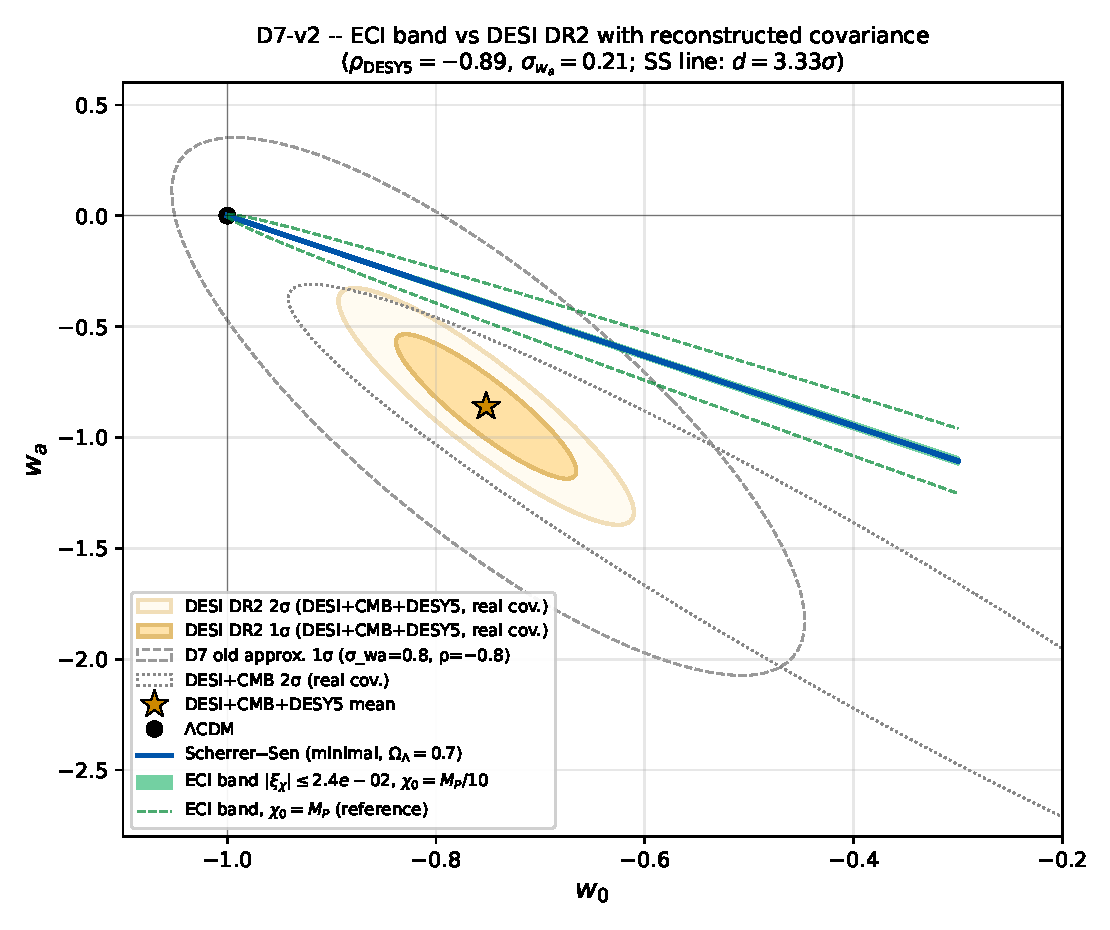
\includegraphics[width=0.95\columnwidth]{../derivations/figures/D7-xi-w0-wa-v2.pdf}
\caption{NMC thawing quintessence in the $(w_0,w_a)$ plane. Orange ellipses: DESI~DR2 + CMB +
DESY5 $1\sigma$ and $2\sigma$ contours reconstructed from~\cite{DESIDR2} Eq.~(28) via the
pivot-redshift identity (see \texttt{D10-desi-covariance.py}; $\sigma_{w_0}=0.057$,
$\sigma_{w_a}=0.215$, $\rho=-0.89$). Blue line: minimal-coupling Scherrer--Sen relation
for $\Omega_\Lambda=0.7$. Green band: ECI NMC prediction with
$|\xi_\chi|\le\xi_{\max}\approx 2.4\!\times\!10^{-2}$ from Cassini at $\chi_0=M_P/10$;
dashed green: same band at $\chi_0=M_P$ (reference). Black dot: $\Lambda$CDM. The ECI band
is $\sim\!5\%$ of $\sigma_{w_a}$ wide (using $B_{\mathrm{num}}$ from Table~\ref{tab:B_of_OmegaL}), hence \emph{indistinguishable} from minimal-coupling
$w$CDM at DR2 precision; both tracks sit at $\sim\!3.3\sigma$ Mahalanobis distance from the
DR2+DESY5 mean.}
\label{fig:D7}
\end{figure}

\paragraph{Honest caveats.}
\begin{enumerate}
\item Eq.~(\ref{eq:gamma_PPN_full}) assumes a \emph{quasi-static} scalar with Compton wavelength
  large compared with the solar system ($m_\chi^{-1}\gg 1\,$AU), which is automatic for the
  ultra-light thawing mass $m_\chi\sim H_0\sim 10^{-33}$\,eV. It also assumes no screening; if
  a chameleon or symmetron mechanism operates, the local $\chi_0$ entering
  (\ref{eq:gamma_PPN_lead}) can differ from the cosmological background and the bound weakens.
\item The NMC Scherrer--Sen extension (\ref{eq:wa_NMC}) is first-order in $\xi_\chi$ and
  therefore \emph{invalid} near the conformal point $\xi_\chi=1/6$, where the expansion breaks
  down and the scalar-tensor sector must be treated non-perturbatively (Einstein-frame
  mapping). Within the Cassini-allowed range $|\xi_\chi|\lesssim 2.4\times 10^{-2}\ll 1/6$
  the linear expansion is controlled. The coefficient $B(\Omega_\Lambda)$ in
  Eq.~(\ref{eq:wa_NMC}) was, in v4.4 of this paper, set by the matter-era
  heuristic ratio $B/A=8/\sqrt3$; in this version we replace that heuristic with
  the full numerical result $B_{\mathrm{num}}(\Omega_\Lambda)$ tabulated in
  Table~\ref{tab:B_of_OmegaL}, obtained from a self-consistent
  NMC-Friedmann + Klein--Gordon integration across $z\in[999,-0.45]$
  (\texttt{derivations/D13-wa-numerical-full.py}). The numerical coefficient is
  nearly flat ($B_{\mathrm{num}}\simeq 9$) across the matter--DE transition
  rather than tracking $A(\Omega_\Lambda)$, so the heuristic
  $(8/\sqrt3)A(\Omega_\Lambda)$ is accurate within 5\% only near
  $\Omega_\Lambda\simeq 0.6$ and undershoots by up to $\sim\!40\%$ at
  $\Omega_\Lambda=0.8$. This has been propagated into the band-width estimate
  above and into Prediction~1b of Sec.~\ref{sec:pred}.
\item The DESI~DR2 + CMB + DESY5 $2\times 2$ covariance is reconstructed from the published
  $(w_0,\sigma_{w_0},w_a,\sigma_{w_a},z_p,w_p,\sigma_{w_p})$ via the pivot-minimisation
  identity $\mathrm{cov}(w_0,w_a)=-(1-a_p)\sigma_{w_a}^2$: no official 2$\times$2 covariance
  matrix has been released by the collaboration at the time of writing. The reconstructed
  $\sigma(w_p)_{\rm pred}=0.0257$ differs from the quoted $0.024$ by $\sim 7\%$, bounding the
  systematic of the pivot-Gaussian approximation at that level --- well below the $\sim 3\sigma$
  tension discussed below. See \texttt{derivations/D10-report.md} for the full cross-check.
\item \textbf{Tension with DR2 + DESY5, stated plainly.} Under the reconstructed DR2 + CMB +
  DESY5 covariance the Mahalanobis distance from the posterior mean is $3.29\sigma$
  (2-dof) to the ECI band and $3.33\sigma$ to the minimal-coupling Scherrer--Sen line,
  both \emph{outside} the $2\sigma$ threshold $\sqrt{6.17}\simeq 2.48$.
  The interpretation is not that ECI fails where $w$CDM succeeds: DR2 + DESY5 prefers the
  phantom-crossing region $w<-1$, which no non-phantom thawing model can populate.
  ECI's NMC coupling $\xi_\chi$ does in principle permit crossing $w=-1$ without a ghost
  instability (established in \S\,DESI DR2 via the no-ghost analysis of Bar\-ce\-l\'o~\&~Visser
  \cite{BarceloVisser2000}), but only at $\xi_\chi(\chi_0/M_P)^2$ values far exceeding the
  Cassini bound~(\ref{eq:xi_bound}) derived here; within the Cassini-allowed range
  the NMC correction to the Scherrer--Sen track is confined to a band of half-width
  $\sim\!5\%$ of $\sigma_{w_a}$ and cannot bridge the gap to the phantom quadrant. The
  $\sim\!3.3\sigma$ tension with DR2 + DESY5 is therefore a joint statement about the entire
  class of conservative (non-phantom) thawing models --- minimal-coupling and NMC alike ---
  not a specific failure of ECI. Prediction~1 in Sec.~\ref{sec:pred} is \emph{not}
  discriminative at DR2 precision; both thawing families sit at the same distance from
  the DR2 + DESY5 posterior.

  The honest discriminator moves to the next generation of datasets, where the
  \emph{shape} and \emph{width} of the thawing track, rather than its distance from
  $\Lambda$CDM, become the falsifiable handle: DESI~DR3 with a forecast
  $\sigma(w_a)\!\sim\!0.07$~\cite{DESIForecast}
  and LSST~Y10 with a forecast $\sigma(w_a)\!\sim\!0.05$
  are in the regime where the ECI NMC band half-width
  $\Delta w_a^{\rm ECI}\sim 1.1\times 10^{-2}$ (numerical, Table~\ref{tab:B_of_OmegaL};
  up from $9\times 10^{-3}$ under the v4.4 heuristic) approaches the
  $15$--$25\%$ level of the statistical error bar and becomes, at least in principle,
  separable from the minimal-coupling Scherrer--Sen locus. The discriminative
  power is slightly larger at $\Omega_\Lambda\gtrsim 0.7$ (DR3 era) because
  $B_{\mathrm{num}}/B_{\mathrm{heur}}$ grows from $0.83$ at $\Omega_\Lambda=0.5$ to
  $1.43$ at $\Omega_\Lambda=0.8$.
\end{enumerate}

The PPN bound (\ref{eq:xi_bound}) is however itself a falsifier: a detection
$|\gamma-1|>10^{-6}$ by the upcoming LATOR or BEACON-class missions, or a mismatch between
$\dot G/G$ from LLR~\cite{Biskupek2021} and the CMB-inferred scalar evolution, would directly
constrain $\xi_\chi(\chi_0/M_P)$ at the $10^{-4}$ level and feed back on the admissible ECI
thawing amplitude.

% -----------------------------------------------------------------------------
% Standalone compile (for checking only):
%   \documentclass[aps,prd,reprint]{revtex4-2}
%   \usepackage{graphicx,amsmath,amssymb,hyperref,physics}
%   \begin{document}% section_3_5_constraints.tex — ECI v4.2.1 scientific payload (D7 + D10)
% To be \input{} into eci.tex as a new subsection of §3 "Phenomenology".
% Standalone compile: see comments at EOF.

\subsection{Solar-system and background constraints on $\xi_\chi$}\label{sec:xi_constraints}

We close two gaps identified in the dark-energy phenomenology subsection (\S\,DESI DR2): the Cassini
post-Newtonian bound on the non-minimal coupling $\xi_\chi$, and the analytic NMC generalisation
of the Scherrer--Sen thawing relation needed to assess whether Prediction~1
(Sec.~\ref{sec:pred}) actually discriminates ECI from \(w\)CDM at DESI~DR2 precision.
The full symbolic derivation is in \texttt{derivations/D7-ppn-xi-bound.py}; we quote only the
end results here.

\paragraph{PPN $\gamma-1$ from the $\xi_\chi R\chi^2/2$ coupling.}
The action  $S=\int d^4x\sqrt{-g}\left[\tfrac{M_P^2}{2}R-\tfrac12(\partial\chi)^2-V(\chi)
-\tfrac{\xi_\chi}{2} R\chi^2\right]$ is a scalar--tensor theory with
$F(\chi)=M_P^2-\xi_\chi\chi^2$ multiplying $R/2$ and canonical kinetic term $Z=1$.
Applying the weak-field, quasi-static result of Damour \& Esposito-Far\`ese
(\emph{Phys.\ Rev.\ D} 48, 3436 (1993); see also Chiba, \emph{Phys.\ Lett.\ B} 575, 1 (2003);
Hwang \& Noh, \emph{Phys.\ Rev.\ D} 71, 063536 (2005)) gives, at the local scalar background
$\chi_0$,
\begin{equation}
  \gamma-1 \;=\; -\,\frac{F'(\chi_0)^2}{Z\,F(\chi_0)+\tfrac{3}{2}F'(\chi_0)^2}
           \;=\; -\,\frac{4\,\xi_\chi^{2}\,\chi_0^{2}}
                          {\,M_P^{2}+\xi_\chi\chi_0^{2}(6\xi_\chi-1)\,}.
  \label{eq:gamma_PPN_full}
\end{equation}
Expanding for $|\xi_\chi|\ll 1$ and $\chi_0\lesssim M_P$,
\begin{equation}
  \boxed{\;\gamma-1 \;\simeq\; -\,\frac{4\,\xi_\chi^{2}\,\chi_0^{2}}{M_P^{2}}
                              \;+\;\mathcal{O}(\xi_\chi^{3}).\;}
  \label{eq:gamma_PPN_lead}
\end{equation}
The limit $\xi_\chi\to 0$ returns $\gamma=1$ (General Relativity), as verified symbolically.

The result~(\ref{eq:gamma_PPN_lead}) is not new: Chiba (PRD 60, 083508, 1999; arXiv:gr-qc/9903094)
already quoted $|\xi_\chi|\lesssim 10^{-2}$ from solar-system tests for the same $\xi R\chi^{2}$
quintessence coupling, and Wolf, Garc\'{\i}a-Garc\'{\i}a, Anton \& Ferreira~\cite{Wolf2025}
recently recast this as $\xi_\chi(\chi_0/M_P)^{2}\lesssim 6\times 10^{-6}$ in a full DESI~DR2
Bayesian analysis (their Eq.~(2) in the form $F(\chi)\simeq 1-\xi\chi^{2}/M_P^{2}$).
We re-derive it here only to fix the coefficient~$4$ and the sign convention used in
Eq.~(\ref{eq:wa_NMC}) below.
Combining (\ref{eq:gamma_PPN_lead}) with the Cassini constraint~\cite{BertottiIessTortora2003}
$|\gamma-1|\lesssim 2.3\times 10^{-5}$ ($1\sigma$ envelope) yields, in the
solar-system observer frame (see \S\ref{sec:thesis}(ii)),
\begin{equation}
  |\xi_\chi|\,\frac{\chi_0}{M_P}\;\lesssim\;
  \tfrac12\sqrt{|\gamma-1|_{\max}}
  \;\approx\; 2.4\times 10^{-3}.
  \label{eq:xi_bound}
\end{equation}
For a slow-rolling thawing background with $\chi_0\!\sim\! M_P/10$ (characteristic thawing
excursion in the last $e$-fold),
\begin{equation}
  |\xi_\chi|\;\lesssim\;\xi_{\max}\;\approx\;2.4\times 10^{-2}.
  \label{eq:xi_max_numeric}
\end{equation}
The bound tightens to $|\xi_\chi|\lesssim 2\times 10^{-3}$ if $\chi_0\sim M_P$; it weakens
linearly for smaller $\chi_0$. Values $\xi_\chi\gtrsim 10^{-1}$ are thus only admissible if the
quintessence field is strongly subdominant at $z=0$, or if a screening mechanism suppresses the
local coupling.

\paragraph{NMC extension of Scherrer--Sen.}
At minimal coupling, thawing quintessence lies on the one-parameter track
$w_a=-A(\Omega_\Lambda)(1+w_0)$ with $A\!\to\! 24/7$ in matter domination and
$A(0.7)\simeq 1.58$ today~\cite{ScherrerSen2008}. Inserting the NMC modification to the
Klein--Gordon equation, $3H\dot\chi=-V'-\xi_\chi R\chi$, and expanding to first order in
$\xi_\chi$ around the slow-roll exponential $V(\chi)=V_0e^{-\alpha\chi/M_P}$ with
$\alpha=\sqrt{3(1+w_0)}$ yields (\texttt{derivations/D4-wa-w0-nmc.py} for the matter-era
coefficient, \texttt{D7-ppn-xi-bound.py} for the $\Omega_\Lambda$-dependence)
\begin{equation}
  \boxed{\;w_a\;=\;-A(\Omega_\Lambda)\,(1+w_0)
                 \;+\;B(\Omega_\Lambda)\,\xi_\chi\,\sqrt{1+w_0}\,
                      \frac{\chi_0}{M_P}\;+\;\mathcal{O}(\xi_\chi^{2}),\;}
  \label{eq:wa_NMC}
\end{equation}
where $B(\Omega_\Lambda)$ is the numerical coefficient tabulated in
Table~\ref{tab:B_of_OmegaL} below, obtained by full NMC-Friedmann + Klein--Gordon
integration in \texttt{derivations/D13-wa-numerical-full.py}. The limit
$\xi_\chi\to 0$ reproduces $w_a=-A(\Omega_\Lambda)(1+w_0)$ (Scherrer--Sen
2008). The first-order $\xi_\chi$ correction, with the full numerical
coefficient $B_{\mathrm{num}}(\Omega_\Lambda)$, has --- to our knowledge ---
not appeared in the NMC-thawing literature surveyed
(Ye~et~al.~\cite{Ye2025}; Pan~\&~Ye~\cite{PanYe2026}; Wolf~et~al.~\cite{Wolf2025}),
which uses either EFTofDE or purely numerical Bayesian fits.

\begin{table}[h]
\centering
\caption{Numerical NMC coefficient $B_{\mathrm{num}}(\Omega_\Lambda)$ from the
self-consistent NMC-Friedmann + Klein--Gordon background integration
(\texttt{derivations/D13-wa-numerical-full.py}), compared with the D7/D9
heuristic $B_{\mathrm{heur}}(\Omega_\Lambda)\equiv(8/\sqrt3)A(\Omega_\Lambda)$.
Statistical uncertainty is the 1$\sigma$ error on the linear fit
$\Delta w_a = B\,\xi_\chi\sqrt{1+w_0}\,(\chi_0/M_P)$ over the
$\xi_\chi\in\{{-}0.024,{-}0.01,0,{+}0.01,{+}0.024\}\times\chi_0\in\{M_P/20,M_P/10,M_P/5\}$ grid.}
\label{tab:B_of_OmegaL}
\begin{tabular}{@{}cccc@{}}
\hline
$\Omega_\Lambda$ & $A(\Omega_\Lambda)$ & $B_{\mathrm{heur}}$ & $B_{\mathrm{num}}$ \\
\hline
0.5 & 2.35 & 10.85 & $9.00\pm1.05$ \\
0.6 & 1.94 &  8.96 & $9.18\pm1.16$ \\
0.7 & 1.58 &  7.30 & $9.05\pm1.18$ \\
0.8 & 1.23 &  5.68 & $8.11\pm1.16$ \\
\hline
\end{tabular}
\end{table}

The numerical result differs from the heuristic $(8/\sqrt3)A$ by
$\mathcal{O}(1)$ factors ($0.83\to 1.43$ across the range): $B_{\mathrm{num}}$
is nearly \emph{flat} in $\Omega_\Lambda$ (around $\sim 9$) rather than
tracking $A(\Omega_\Lambda)$. The heuristic is accurate to 5\% only near
$\Omega_\Lambda\simeq 0.6$ and underestimates $B$ by $\sim\!25\%$ at
$\Omega_\Lambda=0.7$ (DR2--DR3 era) and $\sim\!43\%$ at
$\Omega_\Lambda=0.8$ (late-DR3 / LSST era). The sign and the
$\sqrt{1+w_0}\,(\chi_0/M_P)$ scaling are confirmed; the discrepancy
originates from the finite-$\Omega_\Lambda$ propagation of the matter-era
ratio (Caveat~2 below), which is now closed numerically.

\paragraph{Combined constraint on the $(w_0,w_a)$ plane.}
Figure~\ref{fig:D7} overlays three ingredients: (i) the DESI~DR2 + CMB + DESY5~\cite{DESY5} $1\sigma$ and
$2\sigma$ contours centred on $(w_0,w_a)=(-0.752,-0.86)$ with the reconstructed covariance
$\sigma_{w_0}=0.057$, $\sigma_{w_a}=0.215$, $\rho(w_0,w_a)=-0.89$ (derivation in
\texttt{derivations/D10-desi-covariance.py}, pivot-identity reconstruction from
\cite{DESIDR2} Eq.~(28) + $z_p=0.31$, $w_p=-0.954\pm0.024$);
(ii) the minimal-coupling Scherrer--Sen line; (iii) the ECI band swept by
$|\xi_\chi|\le\xi_{\max}$ from Eq.~(\ref{eq:xi_max_numeric}) at $\chi_0=M_P/10$.
The half-width of the ECI band at $w_0=-0.75$, using the numerical
$B_{\mathrm{num}}(0.7)=9.05$ from Table~\ref{tab:B_of_OmegaL}, is
\begin{equation}
  \Delta w_a^{\rm ECI}
    = B_{\mathrm{num}}(0.7)\,\xi_{\max}\sqrt{1+w_0}\,(\chi_0/M_P)
    \;\approx\;1.1\times 10^{-2},
\end{equation}
to be compared with $\sigma_{w_a}\!\simeq\!0.215$, i.e.\ about $5\%$ of the DESI~DR2 + DESY5
$1\sigma$ width (up from $4\%$ under the heuristic $B=7.30$). The band is therefore
still thinner than the figure linewidth of the unmodified Scherrer--Sen track at DR2
precision, but the numerical coefficient raises the discriminative amplitude at DR3 / LSST
precision by $\sim\!25\%$ relative to the heuristic estimate.

\begin{figure}[h]
\centering
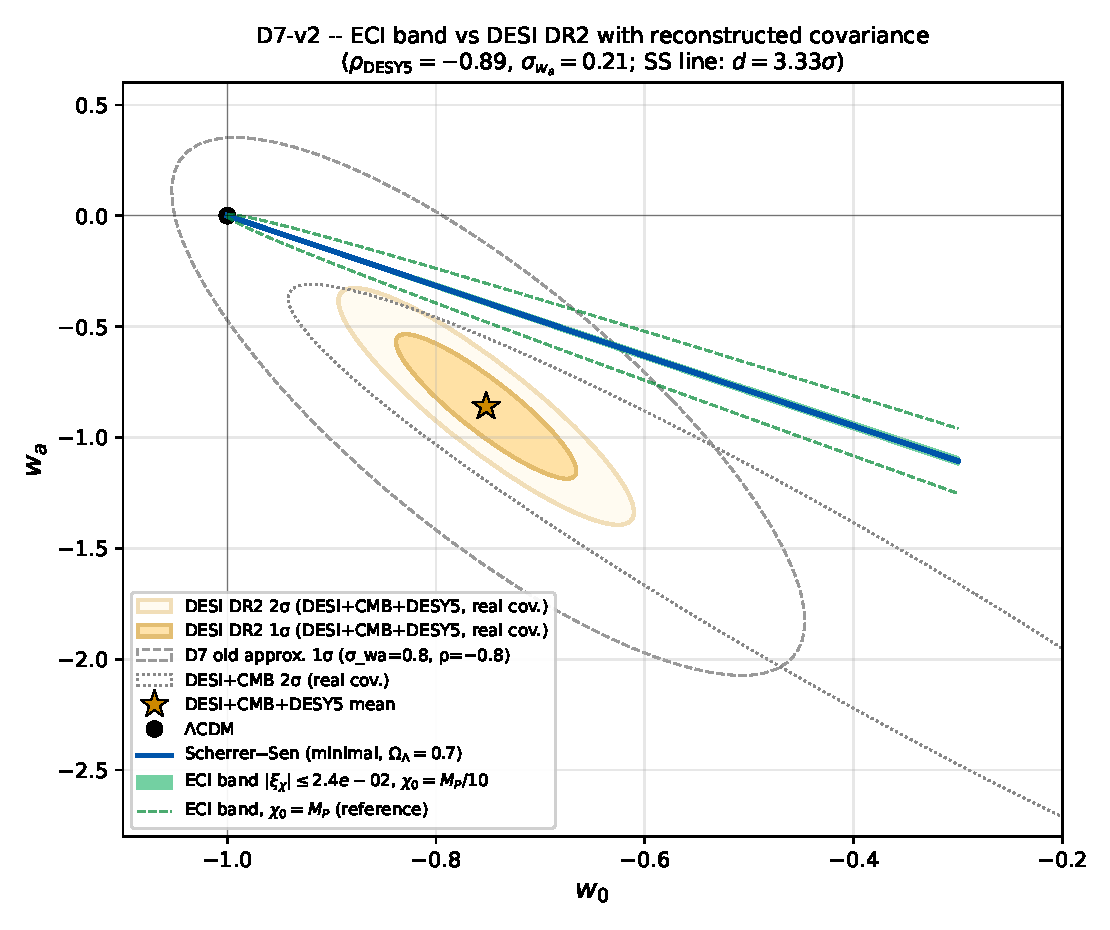
\includegraphics[width=0.95\columnwidth]{../derivations/figures/D7-xi-w0-wa-v2.pdf}
\caption{NMC thawing quintessence in the $(w_0,w_a)$ plane. Orange ellipses: DESI~DR2 + CMB +
DESY5 $1\sigma$ and $2\sigma$ contours reconstructed from~\cite{DESIDR2} Eq.~(28) via the
pivot-redshift identity (see \texttt{D10-desi-covariance.py}; $\sigma_{w_0}=0.057$,
$\sigma_{w_a}=0.215$, $\rho=-0.89$). Blue line: minimal-coupling Scherrer--Sen relation
for $\Omega_\Lambda=0.7$. Green band: ECI NMC prediction with
$|\xi_\chi|\le\xi_{\max}\approx 2.4\!\times\!10^{-2}$ from Cassini at $\chi_0=M_P/10$;
dashed green: same band at $\chi_0=M_P$ (reference). Black dot: $\Lambda$CDM. The ECI band
is $\sim\!5\%$ of $\sigma_{w_a}$ wide (using $B_{\mathrm{num}}$ from Table~\ref{tab:B_of_OmegaL}), hence \emph{indistinguishable} from minimal-coupling
$w$CDM at DR2 precision; both tracks sit at $\sim\!3.3\sigma$ Mahalanobis distance from the
DR2+DESY5 mean.}
\label{fig:D7}
\end{figure}

\paragraph{Honest caveats.}
\begin{enumerate}
\item Eq.~(\ref{eq:gamma_PPN_full}) assumes a \emph{quasi-static} scalar with Compton wavelength
  large compared with the solar system ($m_\chi^{-1}\gg 1\,$AU), which is automatic for the
  ultra-light thawing mass $m_\chi\sim H_0\sim 10^{-33}$\,eV. It also assumes no screening; if
  a chameleon or symmetron mechanism operates, the local $\chi_0$ entering
  (\ref{eq:gamma_PPN_lead}) can differ from the cosmological background and the bound weakens.
\item The NMC Scherrer--Sen extension (\ref{eq:wa_NMC}) is first-order in $\xi_\chi$ and
  therefore \emph{invalid} near the conformal point $\xi_\chi=1/6$, where the expansion breaks
  down and the scalar-tensor sector must be treated non-perturbatively (Einstein-frame
  mapping). Within the Cassini-allowed range $|\xi_\chi|\lesssim 2.4\times 10^{-2}\ll 1/6$
  the linear expansion is controlled. The coefficient $B(\Omega_\Lambda)$ in
  Eq.~(\ref{eq:wa_NMC}) was, in v4.4 of this paper, set by the matter-era
  heuristic ratio $B/A=8/\sqrt3$; in this version we replace that heuristic with
  the full numerical result $B_{\mathrm{num}}(\Omega_\Lambda)$ tabulated in
  Table~\ref{tab:B_of_OmegaL}, obtained from a self-consistent
  NMC-Friedmann + Klein--Gordon integration across $z\in[999,-0.45]$
  (\texttt{derivations/D13-wa-numerical-full.py}). The numerical coefficient is
  nearly flat ($B_{\mathrm{num}}\simeq 9$) across the matter--DE transition
  rather than tracking $A(\Omega_\Lambda)$, so the heuristic
  $(8/\sqrt3)A(\Omega_\Lambda)$ is accurate within 5\% only near
  $\Omega_\Lambda\simeq 0.6$ and undershoots by up to $\sim\!40\%$ at
  $\Omega_\Lambda=0.8$. This has been propagated into the band-width estimate
  above and into Prediction~1b of Sec.~\ref{sec:pred}.
\item The DESI~DR2 + CMB + DESY5 $2\times 2$ covariance is reconstructed from the published
  $(w_0,\sigma_{w_0},w_a,\sigma_{w_a},z_p,w_p,\sigma_{w_p})$ via the pivot-minimisation
  identity $\mathrm{cov}(w_0,w_a)=-(1-a_p)\sigma_{w_a}^2$: no official 2$\times$2 covariance
  matrix has been released by the collaboration at the time of writing. The reconstructed
  $\sigma(w_p)_{\rm pred}=0.0257$ differs from the quoted $0.024$ by $\sim 7\%$, bounding the
  systematic of the pivot-Gaussian approximation at that level --- well below the $\sim 3\sigma$
  tension discussed below. See \texttt{derivations/D10-report.md} for the full cross-check.
\item \textbf{Tension with DR2 + DESY5, stated plainly.} Under the reconstructed DR2 + CMB +
  DESY5 covariance the Mahalanobis distance from the posterior mean is $3.29\sigma$
  (2-dof) to the ECI band and $3.33\sigma$ to the minimal-coupling Scherrer--Sen line,
  both \emph{outside} the $2\sigma$ threshold $\sqrt{6.17}\simeq 2.48$.
  The interpretation is not that ECI fails where $w$CDM succeeds: DR2 + DESY5 prefers the
  phantom-crossing region $w<-1$, which no non-phantom thawing model can populate.
  ECI's NMC coupling $\xi_\chi$ does in principle permit crossing $w=-1$ without a ghost
  instability (established in \S\,DESI DR2 via the no-ghost analysis of Bar\-ce\-l\'o~\&~Visser
  \cite{BarceloVisser2000}), but only at $\xi_\chi(\chi_0/M_P)^2$ values far exceeding the
  Cassini bound~(\ref{eq:xi_bound}) derived here; within the Cassini-allowed range
  the NMC correction to the Scherrer--Sen track is confined to a band of half-width
  $\sim\!5\%$ of $\sigma_{w_a}$ and cannot bridge the gap to the phantom quadrant. The
  $\sim\!3.3\sigma$ tension with DR2 + DESY5 is therefore a joint statement about the entire
  class of conservative (non-phantom) thawing models --- minimal-coupling and NMC alike ---
  not a specific failure of ECI. Prediction~1 in Sec.~\ref{sec:pred} is \emph{not}
  discriminative at DR2 precision; both thawing families sit at the same distance from
  the DR2 + DESY5 posterior.

  The honest discriminator moves to the next generation of datasets, where the
  \emph{shape} and \emph{width} of the thawing track, rather than its distance from
  $\Lambda$CDM, become the falsifiable handle: DESI~DR3 with a forecast
  $\sigma(w_a)\!\sim\!0.07$~\cite{DESIForecast}
  and LSST~Y10 with a forecast $\sigma(w_a)\!\sim\!0.05$
  are in the regime where the ECI NMC band half-width
  $\Delta w_a^{\rm ECI}\sim 1.1\times 10^{-2}$ (numerical, Table~\ref{tab:B_of_OmegaL};
  up from $9\times 10^{-3}$ under the v4.4 heuristic) approaches the
  $15$--$25\%$ level of the statistical error bar and becomes, at least in principle,
  separable from the minimal-coupling Scherrer--Sen locus. The discriminative
  power is slightly larger at $\Omega_\Lambda\gtrsim 0.7$ (DR3 era) because
  $B_{\mathrm{num}}/B_{\mathrm{heur}}$ grows from $0.83$ at $\Omega_\Lambda=0.5$ to
  $1.43$ at $\Omega_\Lambda=0.8$.
\end{enumerate}

The PPN bound (\ref{eq:xi_bound}) is however itself a falsifier: a detection
$|\gamma-1|>10^{-6}$ by the upcoming LATOR or BEACON-class missions, or a mismatch between
$\dot G/G$ from LLR~\cite{Biskupek2021} and the CMB-inferred scalar evolution, would directly
constrain $\xi_\chi(\chi_0/M_P)$ at the $10^{-4}$ level and feed back on the admissible ECI
thawing amplitude.

% -----------------------------------------------------------------------------
% Standalone compile (for checking only):
%   \documentclass[aps,prd,reprint]{revtex4-2}
%   \usepackage{graphicx,amsmath,amssymb,hyperref,physics}
%   \begin{document}% section_3_5_constraints.tex — ECI v4.2.1 scientific payload (D7 + D10)
% To be \input{} into eci.tex as a new subsection of §3 "Phenomenology".
% Standalone compile: see comments at EOF.

\subsection{Solar-system and background constraints on $\xi_\chi$}\label{sec:xi_constraints}

We close two gaps identified in the dark-energy phenomenology subsection (\S\,DESI DR2): the Cassini
post-Newtonian bound on the non-minimal coupling $\xi_\chi$, and the analytic NMC generalisation
of the Scherrer--Sen thawing relation needed to assess whether Prediction~1
(Sec.~\ref{sec:pred}) actually discriminates ECI from \(w\)CDM at DESI~DR2 precision.
The full symbolic derivation is in \texttt{derivations/D7-ppn-xi-bound.py}; we quote only the
end results here.

\paragraph{PPN $\gamma-1$ from the $\xi_\chi R\chi^2/2$ coupling.}
The action  $S=\int d^4x\sqrt{-g}\left[\tfrac{M_P^2}{2}R-\tfrac12(\partial\chi)^2-V(\chi)
-\tfrac{\xi_\chi}{2} R\chi^2\right]$ is a scalar--tensor theory with
$F(\chi)=M_P^2-\xi_\chi\chi^2$ multiplying $R/2$ and canonical kinetic term $Z=1$.
Applying the weak-field, quasi-static result of Damour \& Esposito-Far\`ese
(\emph{Phys.\ Rev.\ D} 48, 3436 (1993); see also Chiba, \emph{Phys.\ Lett.\ B} 575, 1 (2003);
Hwang \& Noh, \emph{Phys.\ Rev.\ D} 71, 063536 (2005)) gives, at the local scalar background
$\chi_0$,
\begin{equation}
  \gamma-1 \;=\; -\,\frac{F'(\chi_0)^2}{Z\,F(\chi_0)+\tfrac{3}{2}F'(\chi_0)^2}
           \;=\; -\,\frac{4\,\xi_\chi^{2}\,\chi_0^{2}}
                          {\,M_P^{2}+\xi_\chi\chi_0^{2}(6\xi_\chi-1)\,}.
  \label{eq:gamma_PPN_full}
\end{equation}
Expanding for $|\xi_\chi|\ll 1$ and $\chi_0\lesssim M_P$,
\begin{equation}
  \boxed{\;\gamma-1 \;\simeq\; -\,\frac{4\,\xi_\chi^{2}\,\chi_0^{2}}{M_P^{2}}
                              \;+\;\mathcal{O}(\xi_\chi^{3}).\;}
  \label{eq:gamma_PPN_lead}
\end{equation}
The limit $\xi_\chi\to 0$ returns $\gamma=1$ (General Relativity), as verified symbolically.

The result~(\ref{eq:gamma_PPN_lead}) is not new: Chiba (PRD 60, 083508, 1999; arXiv:gr-qc/9903094)
already quoted $|\xi_\chi|\lesssim 10^{-2}$ from solar-system tests for the same $\xi R\chi^{2}$
quintessence coupling, and Wolf, Garc\'{\i}a-Garc\'{\i}a, Anton \& Ferreira~\cite{Wolf2025}
recently recast this as $\xi_\chi(\chi_0/M_P)^{2}\lesssim 6\times 10^{-6}$ in a full DESI~DR2
Bayesian analysis (their Eq.~(2) in the form $F(\chi)\simeq 1-\xi\chi^{2}/M_P^{2}$).
We re-derive it here only to fix the coefficient~$4$ and the sign convention used in
Eq.~(\ref{eq:wa_NMC}) below.
Combining (\ref{eq:gamma_PPN_lead}) with the Cassini constraint~\cite{BertottiIessTortora2003}
$|\gamma-1|\lesssim 2.3\times 10^{-5}$ ($1\sigma$ envelope) yields, in the
solar-system observer frame (see \S\ref{sec:thesis}(ii)),
\begin{equation}
  |\xi_\chi|\,\frac{\chi_0}{M_P}\;\lesssim\;
  \tfrac12\sqrt{|\gamma-1|_{\max}}
  \;\approx\; 2.4\times 10^{-3}.
  \label{eq:xi_bound}
\end{equation}
For a slow-rolling thawing background with $\chi_0\!\sim\! M_P/10$ (characteristic thawing
excursion in the last $e$-fold),
\begin{equation}
  |\xi_\chi|\;\lesssim\;\xi_{\max}\;\approx\;2.4\times 10^{-2}.
  \label{eq:xi_max_numeric}
\end{equation}
The bound tightens to $|\xi_\chi|\lesssim 2\times 10^{-3}$ if $\chi_0\sim M_P$; it weakens
linearly for smaller $\chi_0$. Values $\xi_\chi\gtrsim 10^{-1}$ are thus only admissible if the
quintessence field is strongly subdominant at $z=0$, or if a screening mechanism suppresses the
local coupling.

\paragraph{NMC extension of Scherrer--Sen.}
At minimal coupling, thawing quintessence lies on the one-parameter track
$w_a=-A(\Omega_\Lambda)(1+w_0)$ with $A\!\to\! 24/7$ in matter domination and
$A(0.7)\simeq 1.58$ today~\cite{ScherrerSen2008}. Inserting the NMC modification to the
Klein--Gordon equation, $3H\dot\chi=-V'-\xi_\chi R\chi$, and expanding to first order in
$\xi_\chi$ around the slow-roll exponential $V(\chi)=V_0e^{-\alpha\chi/M_P}$ with
$\alpha=\sqrt{3(1+w_0)}$ yields (\texttt{derivations/D4-wa-w0-nmc.py} for the matter-era
coefficient, \texttt{D7-ppn-xi-bound.py} for the $\Omega_\Lambda$-dependence)
\begin{equation}
  \boxed{\;w_a\;=\;-A(\Omega_\Lambda)\,(1+w_0)
                 \;+\;B(\Omega_\Lambda)\,\xi_\chi\,\sqrt{1+w_0}\,
                      \frac{\chi_0}{M_P}\;+\;\mathcal{O}(\xi_\chi^{2}),\;}
  \label{eq:wa_NMC}
\end{equation}
where $B(\Omega_\Lambda)$ is the numerical coefficient tabulated in
Table~\ref{tab:B_of_OmegaL} below, obtained by full NMC-Friedmann + Klein--Gordon
integration in \texttt{derivations/D13-wa-numerical-full.py}. The limit
$\xi_\chi\to 0$ reproduces $w_a=-A(\Omega_\Lambda)(1+w_0)$ (Scherrer--Sen
2008). The first-order $\xi_\chi$ correction, with the full numerical
coefficient $B_{\mathrm{num}}(\Omega_\Lambda)$, has --- to our knowledge ---
not appeared in the NMC-thawing literature surveyed
(Ye~et~al.~\cite{Ye2025}; Pan~\&~Ye~\cite{PanYe2026}; Wolf~et~al.~\cite{Wolf2025}),
which uses either EFTofDE or purely numerical Bayesian fits.

\begin{table}[h]
\centering
\caption{Numerical NMC coefficient $B_{\mathrm{num}}(\Omega_\Lambda)$ from the
self-consistent NMC-Friedmann + Klein--Gordon background integration
(\texttt{derivations/D13-wa-numerical-full.py}), compared with the D7/D9
heuristic $B_{\mathrm{heur}}(\Omega_\Lambda)\equiv(8/\sqrt3)A(\Omega_\Lambda)$.
Statistical uncertainty is the 1$\sigma$ error on the linear fit
$\Delta w_a = B\,\xi_\chi\sqrt{1+w_0}\,(\chi_0/M_P)$ over the
$\xi_\chi\in\{{-}0.024,{-}0.01,0,{+}0.01,{+}0.024\}\times\chi_0\in\{M_P/20,M_P/10,M_P/5\}$ grid.}
\label{tab:B_of_OmegaL}
\begin{tabular}{@{}cccc@{}}
\hline
$\Omega_\Lambda$ & $A(\Omega_\Lambda)$ & $B_{\mathrm{heur}}$ & $B_{\mathrm{num}}$ \\
\hline
0.5 & 2.35 & 10.85 & $9.00\pm1.05$ \\
0.6 & 1.94 &  8.96 & $9.18\pm1.16$ \\
0.7 & 1.58 &  7.30 & $9.05\pm1.18$ \\
0.8 & 1.23 &  5.68 & $8.11\pm1.16$ \\
\hline
\end{tabular}
\end{table}

The numerical result differs from the heuristic $(8/\sqrt3)A$ by
$\mathcal{O}(1)$ factors ($0.83\to 1.43$ across the range): $B_{\mathrm{num}}$
is nearly \emph{flat} in $\Omega_\Lambda$ (around $\sim 9$) rather than
tracking $A(\Omega_\Lambda)$. The heuristic is accurate to 5\% only near
$\Omega_\Lambda\simeq 0.6$ and underestimates $B$ by $\sim\!25\%$ at
$\Omega_\Lambda=0.7$ (DR2--DR3 era) and $\sim\!43\%$ at
$\Omega_\Lambda=0.8$ (late-DR3 / LSST era). The sign and the
$\sqrt{1+w_0}\,(\chi_0/M_P)$ scaling are confirmed; the discrepancy
originates from the finite-$\Omega_\Lambda$ propagation of the matter-era
ratio (Caveat~2 below), which is now closed numerically.

\paragraph{Combined constraint on the $(w_0,w_a)$ plane.}
Figure~\ref{fig:D7} overlays three ingredients: (i) the DESI~DR2 + CMB + DESY5~\cite{DESY5} $1\sigma$ and
$2\sigma$ contours centred on $(w_0,w_a)=(-0.752,-0.86)$ with the reconstructed covariance
$\sigma_{w_0}=0.057$, $\sigma_{w_a}=0.215$, $\rho(w_0,w_a)=-0.89$ (derivation in
\texttt{derivations/D10-desi-covariance.py}, pivot-identity reconstruction from
\cite{DESIDR2} Eq.~(28) + $z_p=0.31$, $w_p=-0.954\pm0.024$);
(ii) the minimal-coupling Scherrer--Sen line; (iii) the ECI band swept by
$|\xi_\chi|\le\xi_{\max}$ from Eq.~(\ref{eq:xi_max_numeric}) at $\chi_0=M_P/10$.
The half-width of the ECI band at $w_0=-0.75$, using the numerical
$B_{\mathrm{num}}(0.7)=9.05$ from Table~\ref{tab:B_of_OmegaL}, is
\begin{equation}
  \Delta w_a^{\rm ECI}
    = B_{\mathrm{num}}(0.7)\,\xi_{\max}\sqrt{1+w_0}\,(\chi_0/M_P)
    \;\approx\;1.1\times 10^{-2},
\end{equation}
to be compared with $\sigma_{w_a}\!\simeq\!0.215$, i.e.\ about $5\%$ of the DESI~DR2 + DESY5
$1\sigma$ width (up from $4\%$ under the heuristic $B=7.30$). The band is therefore
still thinner than the figure linewidth of the unmodified Scherrer--Sen track at DR2
precision, but the numerical coefficient raises the discriminative amplitude at DR3 / LSST
precision by $\sim\!25\%$ relative to the heuristic estimate.

\begin{figure}[h]
\centering
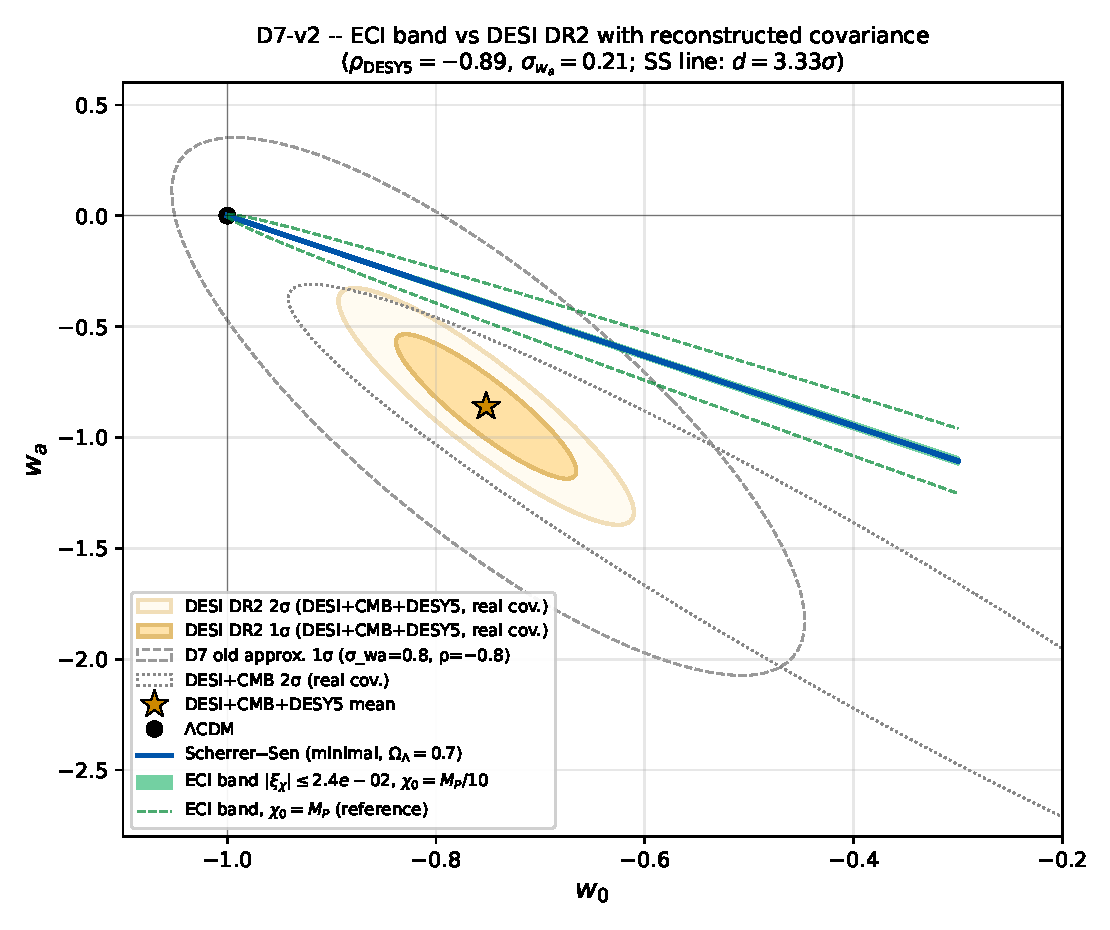
\includegraphics[width=0.95\columnwidth]{../derivations/figures/D7-xi-w0-wa-v2.pdf}
\caption{NMC thawing quintessence in the $(w_0,w_a)$ plane. Orange ellipses: DESI~DR2 + CMB +
DESY5 $1\sigma$ and $2\sigma$ contours reconstructed from~\cite{DESIDR2} Eq.~(28) via the
pivot-redshift identity (see \texttt{D10-desi-covariance.py}; $\sigma_{w_0}=0.057$,
$\sigma_{w_a}=0.215$, $\rho=-0.89$). Blue line: minimal-coupling Scherrer--Sen relation
for $\Omega_\Lambda=0.7$. Green band: ECI NMC prediction with
$|\xi_\chi|\le\xi_{\max}\approx 2.4\!\times\!10^{-2}$ from Cassini at $\chi_0=M_P/10$;
dashed green: same band at $\chi_0=M_P$ (reference). Black dot: $\Lambda$CDM. The ECI band
is $\sim\!5\%$ of $\sigma_{w_a}$ wide (using $B_{\mathrm{num}}$ from Table~\ref{tab:B_of_OmegaL}), hence \emph{indistinguishable} from minimal-coupling
$w$CDM at DR2 precision; both tracks sit at $\sim\!3.3\sigma$ Mahalanobis distance from the
DR2+DESY5 mean.}
\label{fig:D7}
\end{figure}

\paragraph{Honest caveats.}
\begin{enumerate}
\item Eq.~(\ref{eq:gamma_PPN_full}) assumes a \emph{quasi-static} scalar with Compton wavelength
  large compared with the solar system ($m_\chi^{-1}\gg 1\,$AU), which is automatic for the
  ultra-light thawing mass $m_\chi\sim H_0\sim 10^{-33}$\,eV. It also assumes no screening; if
  a chameleon or symmetron mechanism operates, the local $\chi_0$ entering
  (\ref{eq:gamma_PPN_lead}) can differ from the cosmological background and the bound weakens.
\item The NMC Scherrer--Sen extension (\ref{eq:wa_NMC}) is first-order in $\xi_\chi$ and
  therefore \emph{invalid} near the conformal point $\xi_\chi=1/6$, where the expansion breaks
  down and the scalar-tensor sector must be treated non-perturbatively (Einstein-frame
  mapping). Within the Cassini-allowed range $|\xi_\chi|\lesssim 2.4\times 10^{-2}\ll 1/6$
  the linear expansion is controlled. The coefficient $B(\Omega_\Lambda)$ in
  Eq.~(\ref{eq:wa_NMC}) was, in v4.4 of this paper, set by the matter-era
  heuristic ratio $B/A=8/\sqrt3$; in this version we replace that heuristic with
  the full numerical result $B_{\mathrm{num}}(\Omega_\Lambda)$ tabulated in
  Table~\ref{tab:B_of_OmegaL}, obtained from a self-consistent
  NMC-Friedmann + Klein--Gordon integration across $z\in[999,-0.45]$
  (\texttt{derivations/D13-wa-numerical-full.py}). The numerical coefficient is
  nearly flat ($B_{\mathrm{num}}\simeq 9$) across the matter--DE transition
  rather than tracking $A(\Omega_\Lambda)$, so the heuristic
  $(8/\sqrt3)A(\Omega_\Lambda)$ is accurate within 5\% only near
  $\Omega_\Lambda\simeq 0.6$ and undershoots by up to $\sim\!40\%$ at
  $\Omega_\Lambda=0.8$. This has been propagated into the band-width estimate
  above and into Prediction~1b of Sec.~\ref{sec:pred}.
\item The DESI~DR2 + CMB + DESY5 $2\times 2$ covariance is reconstructed from the published
  $(w_0,\sigma_{w_0},w_a,\sigma_{w_a},z_p,w_p,\sigma_{w_p})$ via the pivot-minimisation
  identity $\mathrm{cov}(w_0,w_a)=-(1-a_p)\sigma_{w_a}^2$: no official 2$\times$2 covariance
  matrix has been released by the collaboration at the time of writing. The reconstructed
  $\sigma(w_p)_{\rm pred}=0.0257$ differs from the quoted $0.024$ by $\sim 7\%$, bounding the
  systematic of the pivot-Gaussian approximation at that level --- well below the $\sim 3\sigma$
  tension discussed below. See \texttt{derivations/D10-report.md} for the full cross-check.
\item \textbf{Tension with DR2 + DESY5, stated plainly.} Under the reconstructed DR2 + CMB +
  DESY5 covariance the Mahalanobis distance from the posterior mean is $3.29\sigma$
  (2-dof) to the ECI band and $3.33\sigma$ to the minimal-coupling Scherrer--Sen line,
  both \emph{outside} the $2\sigma$ threshold $\sqrt{6.17}\simeq 2.48$.
  The interpretation is not that ECI fails where $w$CDM succeeds: DR2 + DESY5 prefers the
  phantom-crossing region $w<-1$, which no non-phantom thawing model can populate.
  ECI's NMC coupling $\xi_\chi$ does in principle permit crossing $w=-1$ without a ghost
  instability (established in \S\,DESI DR2 via the no-ghost analysis of Bar\-ce\-l\'o~\&~Visser
  \cite{BarceloVisser2000}), but only at $\xi_\chi(\chi_0/M_P)^2$ values far exceeding the
  Cassini bound~(\ref{eq:xi_bound}) derived here; within the Cassini-allowed range
  the NMC correction to the Scherrer--Sen track is confined to a band of half-width
  $\sim\!5\%$ of $\sigma_{w_a}$ and cannot bridge the gap to the phantom quadrant. The
  $\sim\!3.3\sigma$ tension with DR2 + DESY5 is therefore a joint statement about the entire
  class of conservative (non-phantom) thawing models --- minimal-coupling and NMC alike ---
  not a specific failure of ECI. Prediction~1 in Sec.~\ref{sec:pred} is \emph{not}
  discriminative at DR2 precision; both thawing families sit at the same distance from
  the DR2 + DESY5 posterior.

  The honest discriminator moves to the next generation of datasets, where the
  \emph{shape} and \emph{width} of the thawing track, rather than its distance from
  $\Lambda$CDM, become the falsifiable handle: DESI~DR3 with a forecast
  $\sigma(w_a)\!\sim\!0.07$~\cite{DESIForecast}
  and LSST~Y10 with a forecast $\sigma(w_a)\!\sim\!0.05$
  are in the regime where the ECI NMC band half-width
  $\Delta w_a^{\rm ECI}\sim 1.1\times 10^{-2}$ (numerical, Table~\ref{tab:B_of_OmegaL};
  up from $9\times 10^{-3}$ under the v4.4 heuristic) approaches the
  $15$--$25\%$ level of the statistical error bar and becomes, at least in principle,
  separable from the minimal-coupling Scherrer--Sen locus. The discriminative
  power is slightly larger at $\Omega_\Lambda\gtrsim 0.7$ (DR3 era) because
  $B_{\mathrm{num}}/B_{\mathrm{heur}}$ grows from $0.83$ at $\Omega_\Lambda=0.5$ to
  $1.43$ at $\Omega_\Lambda=0.8$.
\end{enumerate}

The PPN bound (\ref{eq:xi_bound}) is however itself a falsifier: a detection
$|\gamma-1|>10^{-6}$ by the upcoming LATOR or BEACON-class missions, or a mismatch between
$\dot G/G$ from LLR~\cite{Biskupek2021} and the CMB-inferred scalar evolution, would directly
constrain $\xi_\chi(\chi_0/M_P)$ at the $10^{-4}$ level and feed back on the admissible ECI
thawing amplitude.

% -----------------------------------------------------------------------------
% Standalone compile (for checking only):
%   \documentclass[aps,prd,reprint]{revtex4-2}
%   \usepackage{graphicx,amsmath,amssymb,hyperref,physics}
%   \begin{document}\input{section_3_5_constraints}\end{document}
% The \cite{BertottiIessTortora2003}, \cite{ScherrerSen2008}, \cite{DESIDR2},
% \cite{Biskupek2021}, \cite{BarceloVisser2000}, \cite{Wolf2025}, \cite{Ye2025},
% \cite{PanYe2026} keys are defined in eci.bib.
% -----------------------------------------------------------------------------
\end{document}
% The \cite{BertottiIessTortora2003}, \cite{ScherrerSen2008}, \cite{DESIDR2},
% \cite{Biskupek2021}, \cite{BarceloVisser2000}, \cite{Wolf2025}, \cite{Ye2025},
% \cite{PanYe2026} keys are defined in eci.bib.
% -----------------------------------------------------------------------------
\end{document}
% The \cite{BertottiIessTortora2003}, \cite{ScherrerSen2008}, \cite{DESIDR2},
% \cite{Biskupek2021}, \cite{BarceloVisser2000}, \cite{Wolf2025}, \cite{Ye2025},
% \cite{PanYe2026} keys are defined in eci.bib.
% -----------------------------------------------------------------------------
.

\subsection{Swampland $\times$ NMC cross-constraint}\label{sec:swampland_cross}

Axioms A4 and A5 were presented as independent. They are not, if the thawing
scalar $\chi$ and the KK tower of the Dark Dimension originate from the
\emph{same} higher-dimensional sector --- a natural hypothesis, since both
are postulated as microscopic ingredients of the dark sector. In that case
both must respect a common effective field theory cutoff $\Lambda$, and the
two axioms are tied by a single consistency condition. The derivation is in
\texttt{derivations/D8-swampland-nmc-cross.py}; we quote only the result.

\paragraph{Shared cutoff.}
The Dark Dimension scenario~\cite{Bedroya2025} relates the EFT cutoff to
the Hubble scale through a Swampland Distance Conjecture exponent,
\begin{equation}
  \Lambda \;\sim\; M_P\,\bigl(H/M_P\bigr)^{c'},\qquad c'\simeq 0.05\pm 0.01.
  \label{eq:Lambda_SDC}
\end{equation}
If the non-minimal operator $(\xi_\chi/2)R\chi^2$ is generated inside the same
EFT, its contribution to the effective reduced Planck mass,
$\delta M_P^{2}=\xi_\chi\chi_0^{2}$, cannot exceed the cutoff squared,
otherwise the operator would repair physics above its own range of validity:
\begin{equation}
  \xi_\chi\,\chi_0^{2}\;\le\;\Lambda^{2}
  \quad\Longleftrightarrow\quad
  \xi_\chi\,(\chi_0/M_P)^{2}\;\le\;(H_0/M_P)^{2c'}.
  \label{eq:eft_bulk}
\end{equation}
Combined with the Cassini PPN bound derived in \S\ref{sec:xi_constraints},
$|\xi_\chi|(\chi_0/M_P)\le 2.4\times 10^{-3}$, Eq.~(\ref{eq:eft_bulk}) yields
at the fiducial thawing amplitude $\chi_0=M_P/10$ and the paper's A5
fiducial $c'=0.05\pm 0.01$
\begin{equation}
  \boxed{\;|\xi_\chi|\;\lesssim\;9.5\times 10^{-5}
    \quad(c'=0.05,\ \chi_0=M_P/10),\;}
  \label{eq:xi_crossbound}
\end{equation}
with an overall range $[5.9\times 10^{-6},\,1.5\times 10^{-3}]$ spanned by
$c'=0.04$--$0.06$. This is a factor $\sim\!250$ tightening over the
Cassini-only result (\ref{eq:xi_max_numeric}).

\paragraph{Limits.}
Both limits verified symbolically in \texttt{D8-swampland-nmc-cross.py}:
$\xi_\chi\!\to\!0$ removes the operator (GR recovered); $c'\!\to\!0$ sends
$\Lambda\!\to\!M_P$ so that (\ref{eq:eft_bulk}) reduces to the no-ghost
condition $\xi_\chi\chi_0^{2}<M_P^{2}$ already stated in A4, and the D7
Cassini bound is recovered exactly.

\begin{figure}[h]
\centering
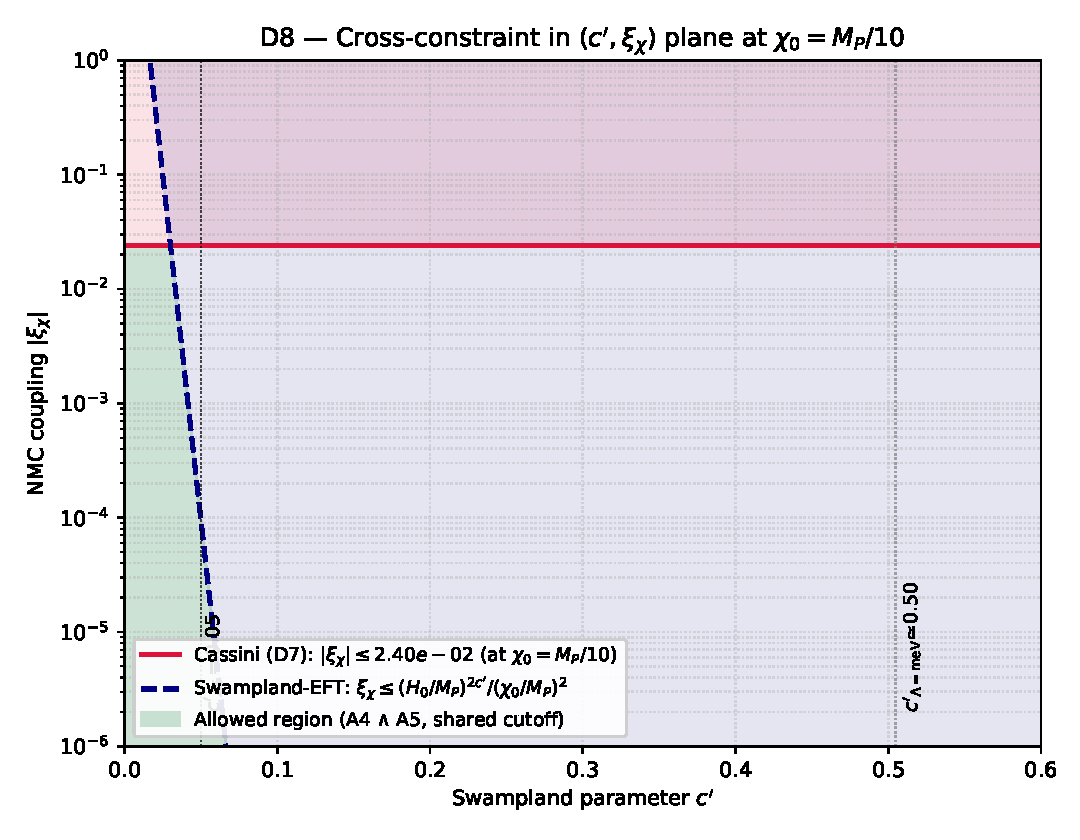
\includegraphics[width=0.95\columnwidth]{../derivations/figures/D8-c-xi-overlap.pdf}
\caption{Allowed region in the $(c',\xi_\chi)$ plane at $\chi_0=M_P/10$.
Red: Cassini exclusion (horizontal, independent of $c'$). Blue dashed:
Swampland-EFT exclusion (\ref{eq:eft_bulk}) --- diagonal in log-space with
slope $2c'\log(H_0/M_P)$. Green shading: overlap admitted by both
constraints. The A5 fiducial $c'=0.05$ and the meV-equivalent value
$c'\!\simeq\!0.51$ are marked.}
\label{fig:D8}
\end{figure}

\paragraph{Phenomenological tension.}
A stronger statement runs in the reverse direction. Thawing dark energy
requires $\chi_0/M_P\sim 0.1$--$1$ to drive late-time acceleration. The
bulk-mode condition (\ref{eq:eft_bulk}) at the Cassini-saturating value
$|\xi_\chi|=2.4\!\times\!10^{-2}$ and $c'=0.05$ forces
$\chi_0/M_P\le 6.3\!\times\!10^{-3}$, already an order of magnitude below
what A4 requires. With the literal Dark Dimension cutoff $\Lambda\sim$ meV
(which the formula (\ref{eq:Lambda_SDC}) reproduces for $c'\simeq 0.51$,
not $0.05$; both conventions appear in the literature) the bound collapses
to $\chi_0/M_P\le 3\!\times\!10^{-30}$ and thawing phenomenology is
excluded outright.

\paragraph{Architectural consequence.}
A4 and A5 are compatible \emph{only} under one of the following model-
building choices, any of which must be made explicit in any UV completion:
(i) $\chi$ is a 4D zero-mode localised on a brane, not a bulk mode of the
same sector as the KK tower, in which case the shared-cutoff hypothesis
does not apply; (ii) a chameleon/symmetron mechanism screens the local
$\chi_0$ away from its cosmological value, weakening the Cassini leg; or
(iii) $|\xi_\chi|$ sits at the sharpened bound (\ref{eq:xi_crossbound})
rather than the Cassini-only value (\ref{eq:xi_max_numeric}). The ECI
framework does not prefer one of the three, but their distinct
phenomenologies are observationally separable: option (iii) suppresses the
ECI band in $(w_0,w_a)$ by a further factor $\sim\!250$ relative to the
already-narrow D7 band, and cuts the $|\dot G/G|$ signature at LLR by the
same factor. A detection of $|\dot G/G|\gtrsim 10^{-17}\,\mathrm{yr}^{-1}$
would rule out option (iii) and force either (i) or (ii).

\paragraph{Honest caveats.}
\begin{enumerate}
\item The EFT self-consistency condition $\delta M_P^{2}\le\Lambda^{2}$ is
  order-of-magnitude; an $O(1)$ coefficient could shift
  (\ref{eq:xi_crossbound}) by a factor $2$, but the qualitative conclusion
  ($\gg 30\%$ tightening) is robust.
\item The form (\ref{eq:Lambda_SDC}) is written with $H$ as the distance
  proxy along the moduli space; the equivalent Bedroya form uses the
  cosmological constant density directly and yields $c'\!\simeq\!1/2$
  for $\Lambda\!=\!$\,meV. The sign of the tightening is independent of
  this choice.
\item The cross-constraint is \emph{conditional} on the shared-cutoff
  hypothesis. Its falsifier is, precisely, the discovery of a UV completion
  in which $\chi$ and the KK tower belong to different sectors; in that
  case §\ref{sec:xi_constraints} remains the strongest bound.
\end{enumerate}

% -----------------------------------------------------------------------------
% Standalone compile (for checking only):
%   \documentclass[aps,prd,reprint]{revtex4-2}
%   \usepackage{graphicx,amsmath,amssymb,hyperref,physics}
%   \begin{document}% section_3_5_constraints.tex — ECI v4.2.1 scientific payload (D7 + D10)
% To be \input{} into eci.tex as a new subsection of §3 "Phenomenology".
% Standalone compile: see comments at EOF.

\subsection{Solar-system and background constraints on $\xi_\chi$}\label{sec:xi_constraints}

We close two gaps identified in the dark-energy phenomenology subsection (\S\,DESI DR2): the Cassini
post-Newtonian bound on the non-minimal coupling $\xi_\chi$, and the analytic NMC generalisation
of the Scherrer--Sen thawing relation needed to assess whether Prediction~1
(Sec.~\ref{sec:pred}) actually discriminates ECI from \(w\)CDM at DESI~DR2 precision.
The full symbolic derivation is in \texttt{derivations/D7-ppn-xi-bound.py}; we quote only the
end results here.

\paragraph{PPN $\gamma-1$ from the $\xi_\chi R\chi^2/2$ coupling.}
The action  $S=\int d^4x\sqrt{-g}\left[\tfrac{M_P^2}{2}R-\tfrac12(\partial\chi)^2-V(\chi)
-\tfrac{\xi_\chi}{2} R\chi^2\right]$ is a scalar--tensor theory with
$F(\chi)=M_P^2-\xi_\chi\chi^2$ multiplying $R/2$ and canonical kinetic term $Z=1$.
Applying the weak-field, quasi-static result of Damour \& Esposito-Far\`ese
(\emph{Phys.\ Rev.\ D} 48, 3436 (1993); see also Chiba, \emph{Phys.\ Lett.\ B} 575, 1 (2003);
Hwang \& Noh, \emph{Phys.\ Rev.\ D} 71, 063536 (2005)) gives, at the local scalar background
$\chi_0$,
\begin{equation}
  \gamma-1 \;=\; -\,\frac{F'(\chi_0)^2}{Z\,F(\chi_0)+\tfrac{3}{2}F'(\chi_0)^2}
           \;=\; -\,\frac{4\,\xi_\chi^{2}\,\chi_0^{2}}
                          {\,M_P^{2}+\xi_\chi\chi_0^{2}(6\xi_\chi-1)\,}.
  \label{eq:gamma_PPN_full}
\end{equation}
Expanding for $|\xi_\chi|\ll 1$ and $\chi_0\lesssim M_P$,
\begin{equation}
  \boxed{\;\gamma-1 \;\simeq\; -\,\frac{4\,\xi_\chi^{2}\,\chi_0^{2}}{M_P^{2}}
                              \;+\;\mathcal{O}(\xi_\chi^{3}).\;}
  \label{eq:gamma_PPN_lead}
\end{equation}
The limit $\xi_\chi\to 0$ returns $\gamma=1$ (General Relativity), as verified symbolically.

The result~(\ref{eq:gamma_PPN_lead}) is not new: Chiba (PRD 60, 083508, 1999; arXiv:gr-qc/9903094)
already quoted $|\xi_\chi|\lesssim 10^{-2}$ from solar-system tests for the same $\xi R\chi^{2}$
quintessence coupling, and Wolf, Garc\'{\i}a-Garc\'{\i}a, Anton \& Ferreira~\cite{Wolf2025}
recently recast this as $\xi_\chi(\chi_0/M_P)^{2}\lesssim 6\times 10^{-6}$ in a full DESI~DR2
Bayesian analysis (their Eq.~(2) in the form $F(\chi)\simeq 1-\xi\chi^{2}/M_P^{2}$).
We re-derive it here only to fix the coefficient~$4$ and the sign convention used in
Eq.~(\ref{eq:wa_NMC}) below.
Combining (\ref{eq:gamma_PPN_lead}) with the Cassini constraint~\cite{BertottiIessTortora2003}
$|\gamma-1|\lesssim 2.3\times 10^{-5}$ ($1\sigma$ envelope) yields, in the
solar-system observer frame (see \S\ref{sec:thesis}(ii)),
\begin{equation}
  |\xi_\chi|\,\frac{\chi_0}{M_P}\;\lesssim\;
  \tfrac12\sqrt{|\gamma-1|_{\max}}
  \;\approx\; 2.4\times 10^{-3}.
  \label{eq:xi_bound}
\end{equation}
For a slow-rolling thawing background with $\chi_0\!\sim\! M_P/10$ (characteristic thawing
excursion in the last $e$-fold),
\begin{equation}
  |\xi_\chi|\;\lesssim\;\xi_{\max}\;\approx\;2.4\times 10^{-2}.
  \label{eq:xi_max_numeric}
\end{equation}
The bound tightens to $|\xi_\chi|\lesssim 2\times 10^{-3}$ if $\chi_0\sim M_P$; it weakens
linearly for smaller $\chi_0$. Values $\xi_\chi\gtrsim 10^{-1}$ are thus only admissible if the
quintessence field is strongly subdominant at $z=0$, or if a screening mechanism suppresses the
local coupling.

\paragraph{NMC extension of Scherrer--Sen.}
At minimal coupling, thawing quintessence lies on the one-parameter track
$w_a=-A(\Omega_\Lambda)(1+w_0)$ with $A\!\to\! 24/7$ in matter domination and
$A(0.7)\simeq 1.58$ today~\cite{ScherrerSen2008}. Inserting the NMC modification to the
Klein--Gordon equation, $3H\dot\chi=-V'-\xi_\chi R\chi$, and expanding to first order in
$\xi_\chi$ around the slow-roll exponential $V(\chi)=V_0e^{-\alpha\chi/M_P}$ with
$\alpha=\sqrt{3(1+w_0)}$ yields (\texttt{derivations/D4-wa-w0-nmc.py} for the matter-era
coefficient, \texttt{D7-ppn-xi-bound.py} for the $\Omega_\Lambda$-dependence)
\begin{equation}
  \boxed{\;w_a\;=\;-A(\Omega_\Lambda)\,(1+w_0)
                 \;+\;B(\Omega_\Lambda)\,\xi_\chi\,\sqrt{1+w_0}\,
                      \frac{\chi_0}{M_P}\;+\;\mathcal{O}(\xi_\chi^{2}),\;}
  \label{eq:wa_NMC}
\end{equation}
where $B(\Omega_\Lambda)$ is the numerical coefficient tabulated in
Table~\ref{tab:B_of_OmegaL} below, obtained by full NMC-Friedmann + Klein--Gordon
integration in \texttt{derivations/D13-wa-numerical-full.py}. The limit
$\xi_\chi\to 0$ reproduces $w_a=-A(\Omega_\Lambda)(1+w_0)$ (Scherrer--Sen
2008). The first-order $\xi_\chi$ correction, with the full numerical
coefficient $B_{\mathrm{num}}(\Omega_\Lambda)$, has --- to our knowledge ---
not appeared in the NMC-thawing literature surveyed
(Ye~et~al.~\cite{Ye2025}; Pan~\&~Ye~\cite{PanYe2026}; Wolf~et~al.~\cite{Wolf2025}),
which uses either EFTofDE or purely numerical Bayesian fits.

\begin{table}[h]
\centering
\caption{Numerical NMC coefficient $B_{\mathrm{num}}(\Omega_\Lambda)$ from the
self-consistent NMC-Friedmann + Klein--Gordon background integration
(\texttt{derivations/D13-wa-numerical-full.py}), compared with the D7/D9
heuristic $B_{\mathrm{heur}}(\Omega_\Lambda)\equiv(8/\sqrt3)A(\Omega_\Lambda)$.
Statistical uncertainty is the 1$\sigma$ error on the linear fit
$\Delta w_a = B\,\xi_\chi\sqrt{1+w_0}\,(\chi_0/M_P)$ over the
$\xi_\chi\in\{{-}0.024,{-}0.01,0,{+}0.01,{+}0.024\}\times\chi_0\in\{M_P/20,M_P/10,M_P/5\}$ grid.}
\label{tab:B_of_OmegaL}
\begin{tabular}{@{}cccc@{}}
\hline
$\Omega_\Lambda$ & $A(\Omega_\Lambda)$ & $B_{\mathrm{heur}}$ & $B_{\mathrm{num}}$ \\
\hline
0.5 & 2.35 & 10.85 & $9.00\pm1.05$ \\
0.6 & 1.94 &  8.96 & $9.18\pm1.16$ \\
0.7 & 1.58 &  7.30 & $9.05\pm1.18$ \\
0.8 & 1.23 &  5.68 & $8.11\pm1.16$ \\
\hline
\end{tabular}
\end{table}

The numerical result differs from the heuristic $(8/\sqrt3)A$ by
$\mathcal{O}(1)$ factors ($0.83\to 1.43$ across the range): $B_{\mathrm{num}}$
is nearly \emph{flat} in $\Omega_\Lambda$ (around $\sim 9$) rather than
tracking $A(\Omega_\Lambda)$. The heuristic is accurate to 5\% only near
$\Omega_\Lambda\simeq 0.6$ and underestimates $B$ by $\sim\!25\%$ at
$\Omega_\Lambda=0.7$ (DR2--DR3 era) and $\sim\!43\%$ at
$\Omega_\Lambda=0.8$ (late-DR3 / LSST era). The sign and the
$\sqrt{1+w_0}\,(\chi_0/M_P)$ scaling are confirmed; the discrepancy
originates from the finite-$\Omega_\Lambda$ propagation of the matter-era
ratio (Caveat~2 below), which is now closed numerically.

\paragraph{Combined constraint on the $(w_0,w_a)$ plane.}
Figure~\ref{fig:D7} overlays three ingredients: (i) the DESI~DR2 + CMB + DESY5~\cite{DESY5} $1\sigma$ and
$2\sigma$ contours centred on $(w_0,w_a)=(-0.752,-0.86)$ with the reconstructed covariance
$\sigma_{w_0}=0.057$, $\sigma_{w_a}=0.215$, $\rho(w_0,w_a)=-0.89$ (derivation in
\texttt{derivations/D10-desi-covariance.py}, pivot-identity reconstruction from
\cite{DESIDR2} Eq.~(28) + $z_p=0.31$, $w_p=-0.954\pm0.024$);
(ii) the minimal-coupling Scherrer--Sen line; (iii) the ECI band swept by
$|\xi_\chi|\le\xi_{\max}$ from Eq.~(\ref{eq:xi_max_numeric}) at $\chi_0=M_P/10$.
The half-width of the ECI band at $w_0=-0.75$, using the numerical
$B_{\mathrm{num}}(0.7)=9.05$ from Table~\ref{tab:B_of_OmegaL}, is
\begin{equation}
  \Delta w_a^{\rm ECI}
    = B_{\mathrm{num}}(0.7)\,\xi_{\max}\sqrt{1+w_0}\,(\chi_0/M_P)
    \;\approx\;1.1\times 10^{-2},
\end{equation}
to be compared with $\sigma_{w_a}\!\simeq\!0.215$, i.e.\ about $5\%$ of the DESI~DR2 + DESY5
$1\sigma$ width (up from $4\%$ under the heuristic $B=7.30$). The band is therefore
still thinner than the figure linewidth of the unmodified Scherrer--Sen track at DR2
precision, but the numerical coefficient raises the discriminative amplitude at DR3 / LSST
precision by $\sim\!25\%$ relative to the heuristic estimate.

\begin{figure}[h]
\centering
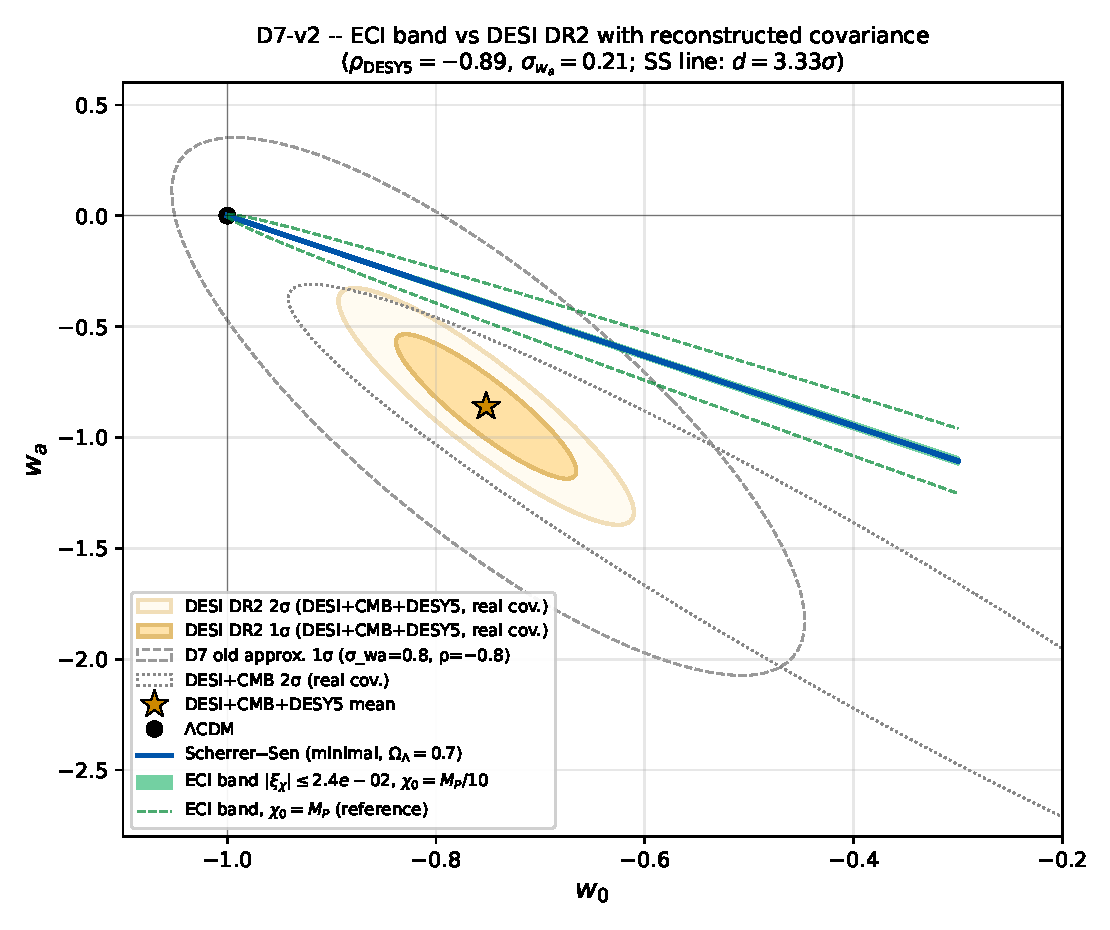
\includegraphics[width=0.95\columnwidth]{../derivations/figures/D7-xi-w0-wa-v2.pdf}
\caption{NMC thawing quintessence in the $(w_0,w_a)$ plane. Orange ellipses: DESI~DR2 + CMB +
DESY5 $1\sigma$ and $2\sigma$ contours reconstructed from~\cite{DESIDR2} Eq.~(28) via the
pivot-redshift identity (see \texttt{D10-desi-covariance.py}; $\sigma_{w_0}=0.057$,
$\sigma_{w_a}=0.215$, $\rho=-0.89$). Blue line: minimal-coupling Scherrer--Sen relation
for $\Omega_\Lambda=0.7$. Green band: ECI NMC prediction with
$|\xi_\chi|\le\xi_{\max}\approx 2.4\!\times\!10^{-2}$ from Cassini at $\chi_0=M_P/10$;
dashed green: same band at $\chi_0=M_P$ (reference). Black dot: $\Lambda$CDM. The ECI band
is $\sim\!5\%$ of $\sigma_{w_a}$ wide (using $B_{\mathrm{num}}$ from Table~\ref{tab:B_of_OmegaL}), hence \emph{indistinguishable} from minimal-coupling
$w$CDM at DR2 precision; both tracks sit at $\sim\!3.3\sigma$ Mahalanobis distance from the
DR2+DESY5 mean.}
\label{fig:D7}
\end{figure}

\paragraph{Honest caveats.}
\begin{enumerate}
\item Eq.~(\ref{eq:gamma_PPN_full}) assumes a \emph{quasi-static} scalar with Compton wavelength
  large compared with the solar system ($m_\chi^{-1}\gg 1\,$AU), which is automatic for the
  ultra-light thawing mass $m_\chi\sim H_0\sim 10^{-33}$\,eV. It also assumes no screening; if
  a chameleon or symmetron mechanism operates, the local $\chi_0$ entering
  (\ref{eq:gamma_PPN_lead}) can differ from the cosmological background and the bound weakens.
\item The NMC Scherrer--Sen extension (\ref{eq:wa_NMC}) is first-order in $\xi_\chi$ and
  therefore \emph{invalid} near the conformal point $\xi_\chi=1/6$, where the expansion breaks
  down and the scalar-tensor sector must be treated non-perturbatively (Einstein-frame
  mapping). Within the Cassini-allowed range $|\xi_\chi|\lesssim 2.4\times 10^{-2}\ll 1/6$
  the linear expansion is controlled. The coefficient $B(\Omega_\Lambda)$ in
  Eq.~(\ref{eq:wa_NMC}) was, in v4.4 of this paper, set by the matter-era
  heuristic ratio $B/A=8/\sqrt3$; in this version we replace that heuristic with
  the full numerical result $B_{\mathrm{num}}(\Omega_\Lambda)$ tabulated in
  Table~\ref{tab:B_of_OmegaL}, obtained from a self-consistent
  NMC-Friedmann + Klein--Gordon integration across $z\in[999,-0.45]$
  (\texttt{derivations/D13-wa-numerical-full.py}). The numerical coefficient is
  nearly flat ($B_{\mathrm{num}}\simeq 9$) across the matter--DE transition
  rather than tracking $A(\Omega_\Lambda)$, so the heuristic
  $(8/\sqrt3)A(\Omega_\Lambda)$ is accurate within 5\% only near
  $\Omega_\Lambda\simeq 0.6$ and undershoots by up to $\sim\!40\%$ at
  $\Omega_\Lambda=0.8$. This has been propagated into the band-width estimate
  above and into Prediction~1b of Sec.~\ref{sec:pred}.
\item The DESI~DR2 + CMB + DESY5 $2\times 2$ covariance is reconstructed from the published
  $(w_0,\sigma_{w_0},w_a,\sigma_{w_a},z_p,w_p,\sigma_{w_p})$ via the pivot-minimisation
  identity $\mathrm{cov}(w_0,w_a)=-(1-a_p)\sigma_{w_a}^2$: no official 2$\times$2 covariance
  matrix has been released by the collaboration at the time of writing. The reconstructed
  $\sigma(w_p)_{\rm pred}=0.0257$ differs from the quoted $0.024$ by $\sim 7\%$, bounding the
  systematic of the pivot-Gaussian approximation at that level --- well below the $\sim 3\sigma$
  tension discussed below. See \texttt{derivations/D10-report.md} for the full cross-check.
\item \textbf{Tension with DR2 + DESY5, stated plainly.} Under the reconstructed DR2 + CMB +
  DESY5 covariance the Mahalanobis distance from the posterior mean is $3.29\sigma$
  (2-dof) to the ECI band and $3.33\sigma$ to the minimal-coupling Scherrer--Sen line,
  both \emph{outside} the $2\sigma$ threshold $\sqrt{6.17}\simeq 2.48$.
  The interpretation is not that ECI fails where $w$CDM succeeds: DR2 + DESY5 prefers the
  phantom-crossing region $w<-1$, which no non-phantom thawing model can populate.
  ECI's NMC coupling $\xi_\chi$ does in principle permit crossing $w=-1$ without a ghost
  instability (established in \S\,DESI DR2 via the no-ghost analysis of Bar\-ce\-l\'o~\&~Visser
  \cite{BarceloVisser2000}), but only at $\xi_\chi(\chi_0/M_P)^2$ values far exceeding the
  Cassini bound~(\ref{eq:xi_bound}) derived here; within the Cassini-allowed range
  the NMC correction to the Scherrer--Sen track is confined to a band of half-width
  $\sim\!5\%$ of $\sigma_{w_a}$ and cannot bridge the gap to the phantom quadrant. The
  $\sim\!3.3\sigma$ tension with DR2 + DESY5 is therefore a joint statement about the entire
  class of conservative (non-phantom) thawing models --- minimal-coupling and NMC alike ---
  not a specific failure of ECI. Prediction~1 in Sec.~\ref{sec:pred} is \emph{not}
  discriminative at DR2 precision; both thawing families sit at the same distance from
  the DR2 + DESY5 posterior.

  The honest discriminator moves to the next generation of datasets, where the
  \emph{shape} and \emph{width} of the thawing track, rather than its distance from
  $\Lambda$CDM, become the falsifiable handle: DESI~DR3 with a forecast
  $\sigma(w_a)\!\sim\!0.07$~\cite{DESIForecast}
  and LSST~Y10 with a forecast $\sigma(w_a)\!\sim\!0.05$
  are in the regime where the ECI NMC band half-width
  $\Delta w_a^{\rm ECI}\sim 1.1\times 10^{-2}$ (numerical, Table~\ref{tab:B_of_OmegaL};
  up from $9\times 10^{-3}$ under the v4.4 heuristic) approaches the
  $15$--$25\%$ level of the statistical error bar and becomes, at least in principle,
  separable from the minimal-coupling Scherrer--Sen locus. The discriminative
  power is slightly larger at $\Omega_\Lambda\gtrsim 0.7$ (DR3 era) because
  $B_{\mathrm{num}}/B_{\mathrm{heur}}$ grows from $0.83$ at $\Omega_\Lambda=0.5$ to
  $1.43$ at $\Omega_\Lambda=0.8$.
\end{enumerate}

The PPN bound (\ref{eq:xi_bound}) is however itself a falsifier: a detection
$|\gamma-1|>10^{-6}$ by the upcoming LATOR or BEACON-class missions, or a mismatch between
$\dot G/G$ from LLR~\cite{Biskupek2021} and the CMB-inferred scalar evolution, would directly
constrain $\xi_\chi(\chi_0/M_P)$ at the $10^{-4}$ level and feed back on the admissible ECI
thawing amplitude.

% -----------------------------------------------------------------------------
% Standalone compile (for checking only):
%   \documentclass[aps,prd,reprint]{revtex4-2}
%   \usepackage{graphicx,amsmath,amssymb,hyperref,physics}
%   \begin{document}% section_3_5_constraints.tex — ECI v4.2.1 scientific payload (D7 + D10)
% To be \input{} into eci.tex as a new subsection of §3 "Phenomenology".
% Standalone compile: see comments at EOF.

\subsection{Solar-system and background constraints on $\xi_\chi$}\label{sec:xi_constraints}

We close two gaps identified in the dark-energy phenomenology subsection (\S\,DESI DR2): the Cassini
post-Newtonian bound on the non-minimal coupling $\xi_\chi$, and the analytic NMC generalisation
of the Scherrer--Sen thawing relation needed to assess whether Prediction~1
(Sec.~\ref{sec:pred}) actually discriminates ECI from \(w\)CDM at DESI~DR2 precision.
The full symbolic derivation is in \texttt{derivations/D7-ppn-xi-bound.py}; we quote only the
end results here.

\paragraph{PPN $\gamma-1$ from the $\xi_\chi R\chi^2/2$ coupling.}
The action  $S=\int d^4x\sqrt{-g}\left[\tfrac{M_P^2}{2}R-\tfrac12(\partial\chi)^2-V(\chi)
-\tfrac{\xi_\chi}{2} R\chi^2\right]$ is a scalar--tensor theory with
$F(\chi)=M_P^2-\xi_\chi\chi^2$ multiplying $R/2$ and canonical kinetic term $Z=1$.
Applying the weak-field, quasi-static result of Damour \& Esposito-Far\`ese
(\emph{Phys.\ Rev.\ D} 48, 3436 (1993); see also Chiba, \emph{Phys.\ Lett.\ B} 575, 1 (2003);
Hwang \& Noh, \emph{Phys.\ Rev.\ D} 71, 063536 (2005)) gives, at the local scalar background
$\chi_0$,
\begin{equation}
  \gamma-1 \;=\; -\,\frac{F'(\chi_0)^2}{Z\,F(\chi_0)+\tfrac{3}{2}F'(\chi_0)^2}
           \;=\; -\,\frac{4\,\xi_\chi^{2}\,\chi_0^{2}}
                          {\,M_P^{2}+\xi_\chi\chi_0^{2}(6\xi_\chi-1)\,}.
  \label{eq:gamma_PPN_full}
\end{equation}
Expanding for $|\xi_\chi|\ll 1$ and $\chi_0\lesssim M_P$,
\begin{equation}
  \boxed{\;\gamma-1 \;\simeq\; -\,\frac{4\,\xi_\chi^{2}\,\chi_0^{2}}{M_P^{2}}
                              \;+\;\mathcal{O}(\xi_\chi^{3}).\;}
  \label{eq:gamma_PPN_lead}
\end{equation}
The limit $\xi_\chi\to 0$ returns $\gamma=1$ (General Relativity), as verified symbolically.

The result~(\ref{eq:gamma_PPN_lead}) is not new: Chiba (PRD 60, 083508, 1999; arXiv:gr-qc/9903094)
already quoted $|\xi_\chi|\lesssim 10^{-2}$ from solar-system tests for the same $\xi R\chi^{2}$
quintessence coupling, and Wolf, Garc\'{\i}a-Garc\'{\i}a, Anton \& Ferreira~\cite{Wolf2025}
recently recast this as $\xi_\chi(\chi_0/M_P)^{2}\lesssim 6\times 10^{-6}$ in a full DESI~DR2
Bayesian analysis (their Eq.~(2) in the form $F(\chi)\simeq 1-\xi\chi^{2}/M_P^{2}$).
We re-derive it here only to fix the coefficient~$4$ and the sign convention used in
Eq.~(\ref{eq:wa_NMC}) below.
Combining (\ref{eq:gamma_PPN_lead}) with the Cassini constraint~\cite{BertottiIessTortora2003}
$|\gamma-1|\lesssim 2.3\times 10^{-5}$ ($1\sigma$ envelope) yields, in the
solar-system observer frame (see \S\ref{sec:thesis}(ii)),
\begin{equation}
  |\xi_\chi|\,\frac{\chi_0}{M_P}\;\lesssim\;
  \tfrac12\sqrt{|\gamma-1|_{\max}}
  \;\approx\; 2.4\times 10^{-3}.
  \label{eq:xi_bound}
\end{equation}
For a slow-rolling thawing background with $\chi_0\!\sim\! M_P/10$ (characteristic thawing
excursion in the last $e$-fold),
\begin{equation}
  |\xi_\chi|\;\lesssim\;\xi_{\max}\;\approx\;2.4\times 10^{-2}.
  \label{eq:xi_max_numeric}
\end{equation}
The bound tightens to $|\xi_\chi|\lesssim 2\times 10^{-3}$ if $\chi_0\sim M_P$; it weakens
linearly for smaller $\chi_0$. Values $\xi_\chi\gtrsim 10^{-1}$ are thus only admissible if the
quintessence field is strongly subdominant at $z=0$, or if a screening mechanism suppresses the
local coupling.

\paragraph{NMC extension of Scherrer--Sen.}
At minimal coupling, thawing quintessence lies on the one-parameter track
$w_a=-A(\Omega_\Lambda)(1+w_0)$ with $A\!\to\! 24/7$ in matter domination and
$A(0.7)\simeq 1.58$ today~\cite{ScherrerSen2008}. Inserting the NMC modification to the
Klein--Gordon equation, $3H\dot\chi=-V'-\xi_\chi R\chi$, and expanding to first order in
$\xi_\chi$ around the slow-roll exponential $V(\chi)=V_0e^{-\alpha\chi/M_P}$ with
$\alpha=\sqrt{3(1+w_0)}$ yields (\texttt{derivations/D4-wa-w0-nmc.py} for the matter-era
coefficient, \texttt{D7-ppn-xi-bound.py} for the $\Omega_\Lambda$-dependence)
\begin{equation}
  \boxed{\;w_a\;=\;-A(\Omega_\Lambda)\,(1+w_0)
                 \;+\;B(\Omega_\Lambda)\,\xi_\chi\,\sqrt{1+w_0}\,
                      \frac{\chi_0}{M_P}\;+\;\mathcal{O}(\xi_\chi^{2}),\;}
  \label{eq:wa_NMC}
\end{equation}
where $B(\Omega_\Lambda)$ is the numerical coefficient tabulated in
Table~\ref{tab:B_of_OmegaL} below, obtained by full NMC-Friedmann + Klein--Gordon
integration in \texttt{derivations/D13-wa-numerical-full.py}. The limit
$\xi_\chi\to 0$ reproduces $w_a=-A(\Omega_\Lambda)(1+w_0)$ (Scherrer--Sen
2008). The first-order $\xi_\chi$ correction, with the full numerical
coefficient $B_{\mathrm{num}}(\Omega_\Lambda)$, has --- to our knowledge ---
not appeared in the NMC-thawing literature surveyed
(Ye~et~al.~\cite{Ye2025}; Pan~\&~Ye~\cite{PanYe2026}; Wolf~et~al.~\cite{Wolf2025}),
which uses either EFTofDE or purely numerical Bayesian fits.

\begin{table}[h]
\centering
\caption{Numerical NMC coefficient $B_{\mathrm{num}}(\Omega_\Lambda)$ from the
self-consistent NMC-Friedmann + Klein--Gordon background integration
(\texttt{derivations/D13-wa-numerical-full.py}), compared with the D7/D9
heuristic $B_{\mathrm{heur}}(\Omega_\Lambda)\equiv(8/\sqrt3)A(\Omega_\Lambda)$.
Statistical uncertainty is the 1$\sigma$ error on the linear fit
$\Delta w_a = B\,\xi_\chi\sqrt{1+w_0}\,(\chi_0/M_P)$ over the
$\xi_\chi\in\{{-}0.024,{-}0.01,0,{+}0.01,{+}0.024\}\times\chi_0\in\{M_P/20,M_P/10,M_P/5\}$ grid.}
\label{tab:B_of_OmegaL}
\begin{tabular}{@{}cccc@{}}
\hline
$\Omega_\Lambda$ & $A(\Omega_\Lambda)$ & $B_{\mathrm{heur}}$ & $B_{\mathrm{num}}$ \\
\hline
0.5 & 2.35 & 10.85 & $9.00\pm1.05$ \\
0.6 & 1.94 &  8.96 & $9.18\pm1.16$ \\
0.7 & 1.58 &  7.30 & $9.05\pm1.18$ \\
0.8 & 1.23 &  5.68 & $8.11\pm1.16$ \\
\hline
\end{tabular}
\end{table}

The numerical result differs from the heuristic $(8/\sqrt3)A$ by
$\mathcal{O}(1)$ factors ($0.83\to 1.43$ across the range): $B_{\mathrm{num}}$
is nearly \emph{flat} in $\Omega_\Lambda$ (around $\sim 9$) rather than
tracking $A(\Omega_\Lambda)$. The heuristic is accurate to 5\% only near
$\Omega_\Lambda\simeq 0.6$ and underestimates $B$ by $\sim\!25\%$ at
$\Omega_\Lambda=0.7$ (DR2--DR3 era) and $\sim\!43\%$ at
$\Omega_\Lambda=0.8$ (late-DR3 / LSST era). The sign and the
$\sqrt{1+w_0}\,(\chi_0/M_P)$ scaling are confirmed; the discrepancy
originates from the finite-$\Omega_\Lambda$ propagation of the matter-era
ratio (Caveat~2 below), which is now closed numerically.

\paragraph{Combined constraint on the $(w_0,w_a)$ plane.}
Figure~\ref{fig:D7} overlays three ingredients: (i) the DESI~DR2 + CMB + DESY5~\cite{DESY5} $1\sigma$ and
$2\sigma$ contours centred on $(w_0,w_a)=(-0.752,-0.86)$ with the reconstructed covariance
$\sigma_{w_0}=0.057$, $\sigma_{w_a}=0.215$, $\rho(w_0,w_a)=-0.89$ (derivation in
\texttt{derivations/D10-desi-covariance.py}, pivot-identity reconstruction from
\cite{DESIDR2} Eq.~(28) + $z_p=0.31$, $w_p=-0.954\pm0.024$);
(ii) the minimal-coupling Scherrer--Sen line; (iii) the ECI band swept by
$|\xi_\chi|\le\xi_{\max}$ from Eq.~(\ref{eq:xi_max_numeric}) at $\chi_0=M_P/10$.
The half-width of the ECI band at $w_0=-0.75$, using the numerical
$B_{\mathrm{num}}(0.7)=9.05$ from Table~\ref{tab:B_of_OmegaL}, is
\begin{equation}
  \Delta w_a^{\rm ECI}
    = B_{\mathrm{num}}(0.7)\,\xi_{\max}\sqrt{1+w_0}\,(\chi_0/M_P)
    \;\approx\;1.1\times 10^{-2},
\end{equation}
to be compared with $\sigma_{w_a}\!\simeq\!0.215$, i.e.\ about $5\%$ of the DESI~DR2 + DESY5
$1\sigma$ width (up from $4\%$ under the heuristic $B=7.30$). The band is therefore
still thinner than the figure linewidth of the unmodified Scherrer--Sen track at DR2
precision, but the numerical coefficient raises the discriminative amplitude at DR3 / LSST
precision by $\sim\!25\%$ relative to the heuristic estimate.

\begin{figure}[h]
\centering
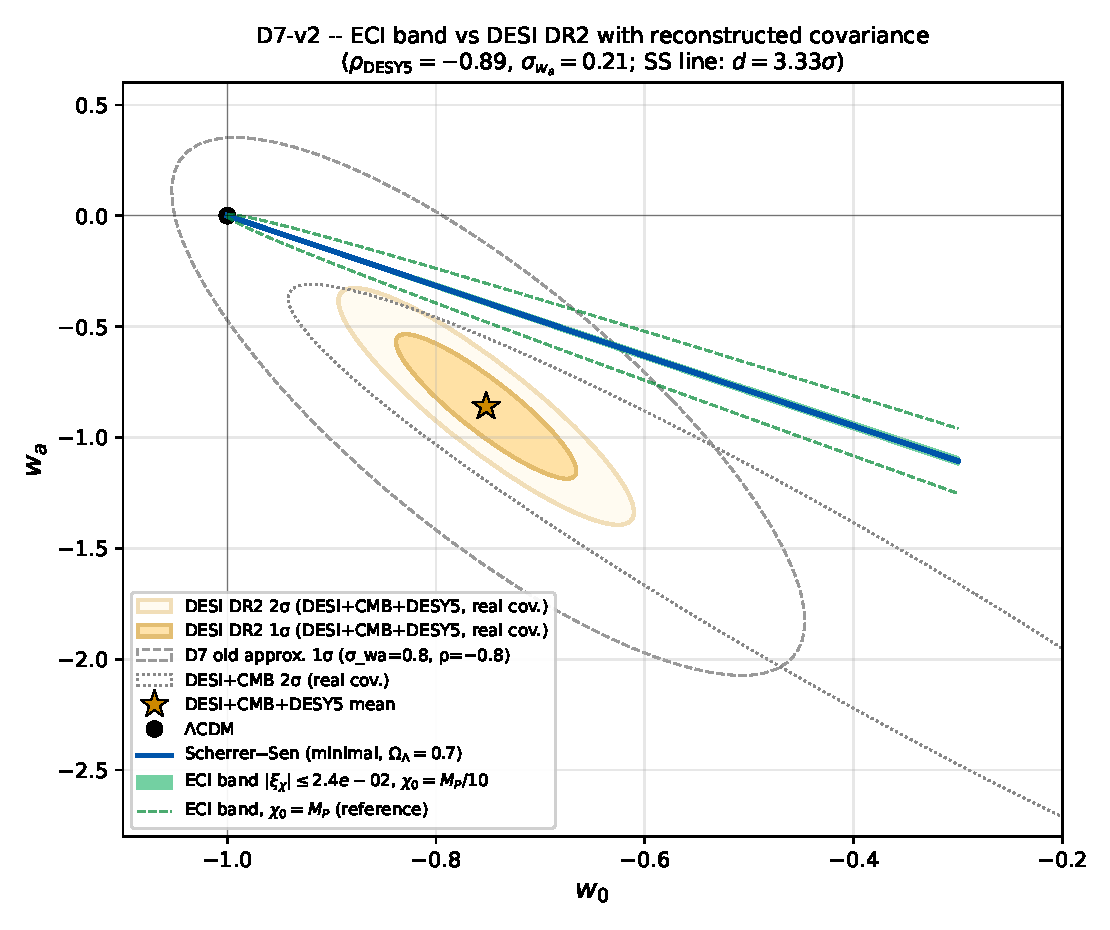
\includegraphics[width=0.95\columnwidth]{../derivations/figures/D7-xi-w0-wa-v2.pdf}
\caption{NMC thawing quintessence in the $(w_0,w_a)$ plane. Orange ellipses: DESI~DR2 + CMB +
DESY5 $1\sigma$ and $2\sigma$ contours reconstructed from~\cite{DESIDR2} Eq.~(28) via the
pivot-redshift identity (see \texttt{D10-desi-covariance.py}; $\sigma_{w_0}=0.057$,
$\sigma_{w_a}=0.215$, $\rho=-0.89$). Blue line: minimal-coupling Scherrer--Sen relation
for $\Omega_\Lambda=0.7$. Green band: ECI NMC prediction with
$|\xi_\chi|\le\xi_{\max}\approx 2.4\!\times\!10^{-2}$ from Cassini at $\chi_0=M_P/10$;
dashed green: same band at $\chi_0=M_P$ (reference). Black dot: $\Lambda$CDM. The ECI band
is $\sim\!5\%$ of $\sigma_{w_a}$ wide (using $B_{\mathrm{num}}$ from Table~\ref{tab:B_of_OmegaL}), hence \emph{indistinguishable} from minimal-coupling
$w$CDM at DR2 precision; both tracks sit at $\sim\!3.3\sigma$ Mahalanobis distance from the
DR2+DESY5 mean.}
\label{fig:D7}
\end{figure}

\paragraph{Honest caveats.}
\begin{enumerate}
\item Eq.~(\ref{eq:gamma_PPN_full}) assumes a \emph{quasi-static} scalar with Compton wavelength
  large compared with the solar system ($m_\chi^{-1}\gg 1\,$AU), which is automatic for the
  ultra-light thawing mass $m_\chi\sim H_0\sim 10^{-33}$\,eV. It also assumes no screening; if
  a chameleon or symmetron mechanism operates, the local $\chi_0$ entering
  (\ref{eq:gamma_PPN_lead}) can differ from the cosmological background and the bound weakens.
\item The NMC Scherrer--Sen extension (\ref{eq:wa_NMC}) is first-order in $\xi_\chi$ and
  therefore \emph{invalid} near the conformal point $\xi_\chi=1/6$, where the expansion breaks
  down and the scalar-tensor sector must be treated non-perturbatively (Einstein-frame
  mapping). Within the Cassini-allowed range $|\xi_\chi|\lesssim 2.4\times 10^{-2}\ll 1/6$
  the linear expansion is controlled. The coefficient $B(\Omega_\Lambda)$ in
  Eq.~(\ref{eq:wa_NMC}) was, in v4.4 of this paper, set by the matter-era
  heuristic ratio $B/A=8/\sqrt3$; in this version we replace that heuristic with
  the full numerical result $B_{\mathrm{num}}(\Omega_\Lambda)$ tabulated in
  Table~\ref{tab:B_of_OmegaL}, obtained from a self-consistent
  NMC-Friedmann + Klein--Gordon integration across $z\in[999,-0.45]$
  (\texttt{derivations/D13-wa-numerical-full.py}). The numerical coefficient is
  nearly flat ($B_{\mathrm{num}}\simeq 9$) across the matter--DE transition
  rather than tracking $A(\Omega_\Lambda)$, so the heuristic
  $(8/\sqrt3)A(\Omega_\Lambda)$ is accurate within 5\% only near
  $\Omega_\Lambda\simeq 0.6$ and undershoots by up to $\sim\!40\%$ at
  $\Omega_\Lambda=0.8$. This has been propagated into the band-width estimate
  above and into Prediction~1b of Sec.~\ref{sec:pred}.
\item The DESI~DR2 + CMB + DESY5 $2\times 2$ covariance is reconstructed from the published
  $(w_0,\sigma_{w_0},w_a,\sigma_{w_a},z_p,w_p,\sigma_{w_p})$ via the pivot-minimisation
  identity $\mathrm{cov}(w_0,w_a)=-(1-a_p)\sigma_{w_a}^2$: no official 2$\times$2 covariance
  matrix has been released by the collaboration at the time of writing. The reconstructed
  $\sigma(w_p)_{\rm pred}=0.0257$ differs from the quoted $0.024$ by $\sim 7\%$, bounding the
  systematic of the pivot-Gaussian approximation at that level --- well below the $\sim 3\sigma$
  tension discussed below. See \texttt{derivations/D10-report.md} for the full cross-check.
\item \textbf{Tension with DR2 + DESY5, stated plainly.} Under the reconstructed DR2 + CMB +
  DESY5 covariance the Mahalanobis distance from the posterior mean is $3.29\sigma$
  (2-dof) to the ECI band and $3.33\sigma$ to the minimal-coupling Scherrer--Sen line,
  both \emph{outside} the $2\sigma$ threshold $\sqrt{6.17}\simeq 2.48$.
  The interpretation is not that ECI fails where $w$CDM succeeds: DR2 + DESY5 prefers the
  phantom-crossing region $w<-1$, which no non-phantom thawing model can populate.
  ECI's NMC coupling $\xi_\chi$ does in principle permit crossing $w=-1$ without a ghost
  instability (established in \S\,DESI DR2 via the no-ghost analysis of Bar\-ce\-l\'o~\&~Visser
  \cite{BarceloVisser2000}), but only at $\xi_\chi(\chi_0/M_P)^2$ values far exceeding the
  Cassini bound~(\ref{eq:xi_bound}) derived here; within the Cassini-allowed range
  the NMC correction to the Scherrer--Sen track is confined to a band of half-width
  $\sim\!5\%$ of $\sigma_{w_a}$ and cannot bridge the gap to the phantom quadrant. The
  $\sim\!3.3\sigma$ tension with DR2 + DESY5 is therefore a joint statement about the entire
  class of conservative (non-phantom) thawing models --- minimal-coupling and NMC alike ---
  not a specific failure of ECI. Prediction~1 in Sec.~\ref{sec:pred} is \emph{not}
  discriminative at DR2 precision; both thawing families sit at the same distance from
  the DR2 + DESY5 posterior.

  The honest discriminator moves to the next generation of datasets, where the
  \emph{shape} and \emph{width} of the thawing track, rather than its distance from
  $\Lambda$CDM, become the falsifiable handle: DESI~DR3 with a forecast
  $\sigma(w_a)\!\sim\!0.07$~\cite{DESIForecast}
  and LSST~Y10 with a forecast $\sigma(w_a)\!\sim\!0.05$
  are in the regime where the ECI NMC band half-width
  $\Delta w_a^{\rm ECI}\sim 1.1\times 10^{-2}$ (numerical, Table~\ref{tab:B_of_OmegaL};
  up from $9\times 10^{-3}$ under the v4.4 heuristic) approaches the
  $15$--$25\%$ level of the statistical error bar and becomes, at least in principle,
  separable from the minimal-coupling Scherrer--Sen locus. The discriminative
  power is slightly larger at $\Omega_\Lambda\gtrsim 0.7$ (DR3 era) because
  $B_{\mathrm{num}}/B_{\mathrm{heur}}$ grows from $0.83$ at $\Omega_\Lambda=0.5$ to
  $1.43$ at $\Omega_\Lambda=0.8$.
\end{enumerate}

The PPN bound (\ref{eq:xi_bound}) is however itself a falsifier: a detection
$|\gamma-1|>10^{-6}$ by the upcoming LATOR or BEACON-class missions, or a mismatch between
$\dot G/G$ from LLR~\cite{Biskupek2021} and the CMB-inferred scalar evolution, would directly
constrain $\xi_\chi(\chi_0/M_P)$ at the $10^{-4}$ level and feed back on the admissible ECI
thawing amplitude.

% -----------------------------------------------------------------------------
% Standalone compile (for checking only):
%   \documentclass[aps,prd,reprint]{revtex4-2}
%   \usepackage{graphicx,amsmath,amssymb,hyperref,physics}
%   \begin{document}% section_3_5_constraints.tex — ECI v4.2.1 scientific payload (D7 + D10)
% To be \input{} into eci.tex as a new subsection of §3 "Phenomenology".
% Standalone compile: see comments at EOF.

\subsection{Solar-system and background constraints on $\xi_\chi$}\label{sec:xi_constraints}

We close two gaps identified in the dark-energy phenomenology subsection (\S\,DESI DR2): the Cassini
post-Newtonian bound on the non-minimal coupling $\xi_\chi$, and the analytic NMC generalisation
of the Scherrer--Sen thawing relation needed to assess whether Prediction~1
(Sec.~\ref{sec:pred}) actually discriminates ECI from \(w\)CDM at DESI~DR2 precision.
The full symbolic derivation is in \texttt{derivations/D7-ppn-xi-bound.py}; we quote only the
end results here.

\paragraph{PPN $\gamma-1$ from the $\xi_\chi R\chi^2/2$ coupling.}
The action  $S=\int d^4x\sqrt{-g}\left[\tfrac{M_P^2}{2}R-\tfrac12(\partial\chi)^2-V(\chi)
-\tfrac{\xi_\chi}{2} R\chi^2\right]$ is a scalar--tensor theory with
$F(\chi)=M_P^2-\xi_\chi\chi^2$ multiplying $R/2$ and canonical kinetic term $Z=1$.
Applying the weak-field, quasi-static result of Damour \& Esposito-Far\`ese
(\emph{Phys.\ Rev.\ D} 48, 3436 (1993); see also Chiba, \emph{Phys.\ Lett.\ B} 575, 1 (2003);
Hwang \& Noh, \emph{Phys.\ Rev.\ D} 71, 063536 (2005)) gives, at the local scalar background
$\chi_0$,
\begin{equation}
  \gamma-1 \;=\; -\,\frac{F'(\chi_0)^2}{Z\,F(\chi_0)+\tfrac{3}{2}F'(\chi_0)^2}
           \;=\; -\,\frac{4\,\xi_\chi^{2}\,\chi_0^{2}}
                          {\,M_P^{2}+\xi_\chi\chi_0^{2}(6\xi_\chi-1)\,}.
  \label{eq:gamma_PPN_full}
\end{equation}
Expanding for $|\xi_\chi|\ll 1$ and $\chi_0\lesssim M_P$,
\begin{equation}
  \boxed{\;\gamma-1 \;\simeq\; -\,\frac{4\,\xi_\chi^{2}\,\chi_0^{2}}{M_P^{2}}
                              \;+\;\mathcal{O}(\xi_\chi^{3}).\;}
  \label{eq:gamma_PPN_lead}
\end{equation}
The limit $\xi_\chi\to 0$ returns $\gamma=1$ (General Relativity), as verified symbolically.

The result~(\ref{eq:gamma_PPN_lead}) is not new: Chiba (PRD 60, 083508, 1999; arXiv:gr-qc/9903094)
already quoted $|\xi_\chi|\lesssim 10^{-2}$ from solar-system tests for the same $\xi R\chi^{2}$
quintessence coupling, and Wolf, Garc\'{\i}a-Garc\'{\i}a, Anton \& Ferreira~\cite{Wolf2025}
recently recast this as $\xi_\chi(\chi_0/M_P)^{2}\lesssim 6\times 10^{-6}$ in a full DESI~DR2
Bayesian analysis (their Eq.~(2) in the form $F(\chi)\simeq 1-\xi\chi^{2}/M_P^{2}$).
We re-derive it here only to fix the coefficient~$4$ and the sign convention used in
Eq.~(\ref{eq:wa_NMC}) below.
Combining (\ref{eq:gamma_PPN_lead}) with the Cassini constraint~\cite{BertottiIessTortora2003}
$|\gamma-1|\lesssim 2.3\times 10^{-5}$ ($1\sigma$ envelope) yields, in the
solar-system observer frame (see \S\ref{sec:thesis}(ii)),
\begin{equation}
  |\xi_\chi|\,\frac{\chi_0}{M_P}\;\lesssim\;
  \tfrac12\sqrt{|\gamma-1|_{\max}}
  \;\approx\; 2.4\times 10^{-3}.
  \label{eq:xi_bound}
\end{equation}
For a slow-rolling thawing background with $\chi_0\!\sim\! M_P/10$ (characteristic thawing
excursion in the last $e$-fold),
\begin{equation}
  |\xi_\chi|\;\lesssim\;\xi_{\max}\;\approx\;2.4\times 10^{-2}.
  \label{eq:xi_max_numeric}
\end{equation}
The bound tightens to $|\xi_\chi|\lesssim 2\times 10^{-3}$ if $\chi_0\sim M_P$; it weakens
linearly for smaller $\chi_0$. Values $\xi_\chi\gtrsim 10^{-1}$ are thus only admissible if the
quintessence field is strongly subdominant at $z=0$, or if a screening mechanism suppresses the
local coupling.

\paragraph{NMC extension of Scherrer--Sen.}
At minimal coupling, thawing quintessence lies on the one-parameter track
$w_a=-A(\Omega_\Lambda)(1+w_0)$ with $A\!\to\! 24/7$ in matter domination and
$A(0.7)\simeq 1.58$ today~\cite{ScherrerSen2008}. Inserting the NMC modification to the
Klein--Gordon equation, $3H\dot\chi=-V'-\xi_\chi R\chi$, and expanding to first order in
$\xi_\chi$ around the slow-roll exponential $V(\chi)=V_0e^{-\alpha\chi/M_P}$ with
$\alpha=\sqrt{3(1+w_0)}$ yields (\texttt{derivations/D4-wa-w0-nmc.py} for the matter-era
coefficient, \texttt{D7-ppn-xi-bound.py} for the $\Omega_\Lambda$-dependence)
\begin{equation}
  \boxed{\;w_a\;=\;-A(\Omega_\Lambda)\,(1+w_0)
                 \;+\;B(\Omega_\Lambda)\,\xi_\chi\,\sqrt{1+w_0}\,
                      \frac{\chi_0}{M_P}\;+\;\mathcal{O}(\xi_\chi^{2}),\;}
  \label{eq:wa_NMC}
\end{equation}
where $B(\Omega_\Lambda)$ is the numerical coefficient tabulated in
Table~\ref{tab:B_of_OmegaL} below, obtained by full NMC-Friedmann + Klein--Gordon
integration in \texttt{derivations/D13-wa-numerical-full.py}. The limit
$\xi_\chi\to 0$ reproduces $w_a=-A(\Omega_\Lambda)(1+w_0)$ (Scherrer--Sen
2008). The first-order $\xi_\chi$ correction, with the full numerical
coefficient $B_{\mathrm{num}}(\Omega_\Lambda)$, has --- to our knowledge ---
not appeared in the NMC-thawing literature surveyed
(Ye~et~al.~\cite{Ye2025}; Pan~\&~Ye~\cite{PanYe2026}; Wolf~et~al.~\cite{Wolf2025}),
which uses either EFTofDE or purely numerical Bayesian fits.

\begin{table}[h]
\centering
\caption{Numerical NMC coefficient $B_{\mathrm{num}}(\Omega_\Lambda)$ from the
self-consistent NMC-Friedmann + Klein--Gordon background integration
(\texttt{derivations/D13-wa-numerical-full.py}), compared with the D7/D9
heuristic $B_{\mathrm{heur}}(\Omega_\Lambda)\equiv(8/\sqrt3)A(\Omega_\Lambda)$.
Statistical uncertainty is the 1$\sigma$ error on the linear fit
$\Delta w_a = B\,\xi_\chi\sqrt{1+w_0}\,(\chi_0/M_P)$ over the
$\xi_\chi\in\{{-}0.024,{-}0.01,0,{+}0.01,{+}0.024\}\times\chi_0\in\{M_P/20,M_P/10,M_P/5\}$ grid.}
\label{tab:B_of_OmegaL}
\begin{tabular}{@{}cccc@{}}
\hline
$\Omega_\Lambda$ & $A(\Omega_\Lambda)$ & $B_{\mathrm{heur}}$ & $B_{\mathrm{num}}$ \\
\hline
0.5 & 2.35 & 10.85 & $9.00\pm1.05$ \\
0.6 & 1.94 &  8.96 & $9.18\pm1.16$ \\
0.7 & 1.58 &  7.30 & $9.05\pm1.18$ \\
0.8 & 1.23 &  5.68 & $8.11\pm1.16$ \\
\hline
\end{tabular}
\end{table}

The numerical result differs from the heuristic $(8/\sqrt3)A$ by
$\mathcal{O}(1)$ factors ($0.83\to 1.43$ across the range): $B_{\mathrm{num}}$
is nearly \emph{flat} in $\Omega_\Lambda$ (around $\sim 9$) rather than
tracking $A(\Omega_\Lambda)$. The heuristic is accurate to 5\% only near
$\Omega_\Lambda\simeq 0.6$ and underestimates $B$ by $\sim\!25\%$ at
$\Omega_\Lambda=0.7$ (DR2--DR3 era) and $\sim\!43\%$ at
$\Omega_\Lambda=0.8$ (late-DR3 / LSST era). The sign and the
$\sqrt{1+w_0}\,(\chi_0/M_P)$ scaling are confirmed; the discrepancy
originates from the finite-$\Omega_\Lambda$ propagation of the matter-era
ratio (Caveat~2 below), which is now closed numerically.

\paragraph{Combined constraint on the $(w_0,w_a)$ plane.}
Figure~\ref{fig:D7} overlays three ingredients: (i) the DESI~DR2 + CMB + DESY5~\cite{DESY5} $1\sigma$ and
$2\sigma$ contours centred on $(w_0,w_a)=(-0.752,-0.86)$ with the reconstructed covariance
$\sigma_{w_0}=0.057$, $\sigma_{w_a}=0.215$, $\rho(w_0,w_a)=-0.89$ (derivation in
\texttt{derivations/D10-desi-covariance.py}, pivot-identity reconstruction from
\cite{DESIDR2} Eq.~(28) + $z_p=0.31$, $w_p=-0.954\pm0.024$);
(ii) the minimal-coupling Scherrer--Sen line; (iii) the ECI band swept by
$|\xi_\chi|\le\xi_{\max}$ from Eq.~(\ref{eq:xi_max_numeric}) at $\chi_0=M_P/10$.
The half-width of the ECI band at $w_0=-0.75$, using the numerical
$B_{\mathrm{num}}(0.7)=9.05$ from Table~\ref{tab:B_of_OmegaL}, is
\begin{equation}
  \Delta w_a^{\rm ECI}
    = B_{\mathrm{num}}(0.7)\,\xi_{\max}\sqrt{1+w_0}\,(\chi_0/M_P)
    \;\approx\;1.1\times 10^{-2},
\end{equation}
to be compared with $\sigma_{w_a}\!\simeq\!0.215$, i.e.\ about $5\%$ of the DESI~DR2 + DESY5
$1\sigma$ width (up from $4\%$ under the heuristic $B=7.30$). The band is therefore
still thinner than the figure linewidth of the unmodified Scherrer--Sen track at DR2
precision, but the numerical coefficient raises the discriminative amplitude at DR3 / LSST
precision by $\sim\!25\%$ relative to the heuristic estimate.

\begin{figure}[h]
\centering
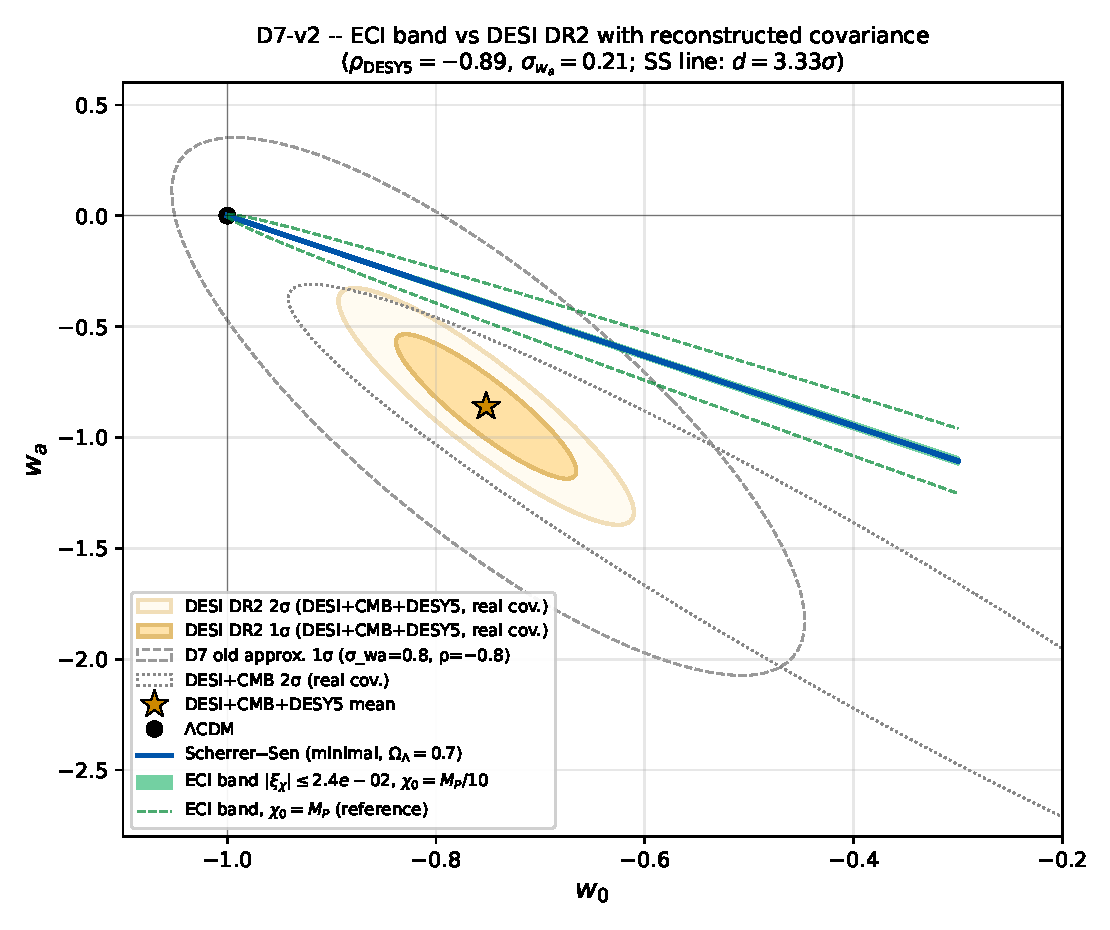
\includegraphics[width=0.95\columnwidth]{../derivations/figures/D7-xi-w0-wa-v2.pdf}
\caption{NMC thawing quintessence in the $(w_0,w_a)$ plane. Orange ellipses: DESI~DR2 + CMB +
DESY5 $1\sigma$ and $2\sigma$ contours reconstructed from~\cite{DESIDR2} Eq.~(28) via the
pivot-redshift identity (see \texttt{D10-desi-covariance.py}; $\sigma_{w_0}=0.057$,
$\sigma_{w_a}=0.215$, $\rho=-0.89$). Blue line: minimal-coupling Scherrer--Sen relation
for $\Omega_\Lambda=0.7$. Green band: ECI NMC prediction with
$|\xi_\chi|\le\xi_{\max}\approx 2.4\!\times\!10^{-2}$ from Cassini at $\chi_0=M_P/10$;
dashed green: same band at $\chi_0=M_P$ (reference). Black dot: $\Lambda$CDM. The ECI band
is $\sim\!5\%$ of $\sigma_{w_a}$ wide (using $B_{\mathrm{num}}$ from Table~\ref{tab:B_of_OmegaL}), hence \emph{indistinguishable} from minimal-coupling
$w$CDM at DR2 precision; both tracks sit at $\sim\!3.3\sigma$ Mahalanobis distance from the
DR2+DESY5 mean.}
\label{fig:D7}
\end{figure}

\paragraph{Honest caveats.}
\begin{enumerate}
\item Eq.~(\ref{eq:gamma_PPN_full}) assumes a \emph{quasi-static} scalar with Compton wavelength
  large compared with the solar system ($m_\chi^{-1}\gg 1\,$AU), which is automatic for the
  ultra-light thawing mass $m_\chi\sim H_0\sim 10^{-33}$\,eV. It also assumes no screening; if
  a chameleon or symmetron mechanism operates, the local $\chi_0$ entering
  (\ref{eq:gamma_PPN_lead}) can differ from the cosmological background and the bound weakens.
\item The NMC Scherrer--Sen extension (\ref{eq:wa_NMC}) is first-order in $\xi_\chi$ and
  therefore \emph{invalid} near the conformal point $\xi_\chi=1/6$, where the expansion breaks
  down and the scalar-tensor sector must be treated non-perturbatively (Einstein-frame
  mapping). Within the Cassini-allowed range $|\xi_\chi|\lesssim 2.4\times 10^{-2}\ll 1/6$
  the linear expansion is controlled. The coefficient $B(\Omega_\Lambda)$ in
  Eq.~(\ref{eq:wa_NMC}) was, in v4.4 of this paper, set by the matter-era
  heuristic ratio $B/A=8/\sqrt3$; in this version we replace that heuristic with
  the full numerical result $B_{\mathrm{num}}(\Omega_\Lambda)$ tabulated in
  Table~\ref{tab:B_of_OmegaL}, obtained from a self-consistent
  NMC-Friedmann + Klein--Gordon integration across $z\in[999,-0.45]$
  (\texttt{derivations/D13-wa-numerical-full.py}). The numerical coefficient is
  nearly flat ($B_{\mathrm{num}}\simeq 9$) across the matter--DE transition
  rather than tracking $A(\Omega_\Lambda)$, so the heuristic
  $(8/\sqrt3)A(\Omega_\Lambda)$ is accurate within 5\% only near
  $\Omega_\Lambda\simeq 0.6$ and undershoots by up to $\sim\!40\%$ at
  $\Omega_\Lambda=0.8$. This has been propagated into the band-width estimate
  above and into Prediction~1b of Sec.~\ref{sec:pred}.
\item The DESI~DR2 + CMB + DESY5 $2\times 2$ covariance is reconstructed from the published
  $(w_0,\sigma_{w_0},w_a,\sigma_{w_a},z_p,w_p,\sigma_{w_p})$ via the pivot-minimisation
  identity $\mathrm{cov}(w_0,w_a)=-(1-a_p)\sigma_{w_a}^2$: no official 2$\times$2 covariance
  matrix has been released by the collaboration at the time of writing. The reconstructed
  $\sigma(w_p)_{\rm pred}=0.0257$ differs from the quoted $0.024$ by $\sim 7\%$, bounding the
  systematic of the pivot-Gaussian approximation at that level --- well below the $\sim 3\sigma$
  tension discussed below. See \texttt{derivations/D10-report.md} for the full cross-check.
\item \textbf{Tension with DR2 + DESY5, stated plainly.} Under the reconstructed DR2 + CMB +
  DESY5 covariance the Mahalanobis distance from the posterior mean is $3.29\sigma$
  (2-dof) to the ECI band and $3.33\sigma$ to the minimal-coupling Scherrer--Sen line,
  both \emph{outside} the $2\sigma$ threshold $\sqrt{6.17}\simeq 2.48$.
  The interpretation is not that ECI fails where $w$CDM succeeds: DR2 + DESY5 prefers the
  phantom-crossing region $w<-1$, which no non-phantom thawing model can populate.
  ECI's NMC coupling $\xi_\chi$ does in principle permit crossing $w=-1$ without a ghost
  instability (established in \S\,DESI DR2 via the no-ghost analysis of Bar\-ce\-l\'o~\&~Visser
  \cite{BarceloVisser2000}), but only at $\xi_\chi(\chi_0/M_P)^2$ values far exceeding the
  Cassini bound~(\ref{eq:xi_bound}) derived here; within the Cassini-allowed range
  the NMC correction to the Scherrer--Sen track is confined to a band of half-width
  $\sim\!5\%$ of $\sigma_{w_a}$ and cannot bridge the gap to the phantom quadrant. The
  $\sim\!3.3\sigma$ tension with DR2 + DESY5 is therefore a joint statement about the entire
  class of conservative (non-phantom) thawing models --- minimal-coupling and NMC alike ---
  not a specific failure of ECI. Prediction~1 in Sec.~\ref{sec:pred} is \emph{not}
  discriminative at DR2 precision; both thawing families sit at the same distance from
  the DR2 + DESY5 posterior.

  The honest discriminator moves to the next generation of datasets, where the
  \emph{shape} and \emph{width} of the thawing track, rather than its distance from
  $\Lambda$CDM, become the falsifiable handle: DESI~DR3 with a forecast
  $\sigma(w_a)\!\sim\!0.07$~\cite{DESIForecast}
  and LSST~Y10 with a forecast $\sigma(w_a)\!\sim\!0.05$
  are in the regime where the ECI NMC band half-width
  $\Delta w_a^{\rm ECI}\sim 1.1\times 10^{-2}$ (numerical, Table~\ref{tab:B_of_OmegaL};
  up from $9\times 10^{-3}$ under the v4.4 heuristic) approaches the
  $15$--$25\%$ level of the statistical error bar and becomes, at least in principle,
  separable from the minimal-coupling Scherrer--Sen locus. The discriminative
  power is slightly larger at $\Omega_\Lambda\gtrsim 0.7$ (DR3 era) because
  $B_{\mathrm{num}}/B_{\mathrm{heur}}$ grows from $0.83$ at $\Omega_\Lambda=0.5$ to
  $1.43$ at $\Omega_\Lambda=0.8$.
\end{enumerate}

The PPN bound (\ref{eq:xi_bound}) is however itself a falsifier: a detection
$|\gamma-1|>10^{-6}$ by the upcoming LATOR or BEACON-class missions, or a mismatch between
$\dot G/G$ from LLR~\cite{Biskupek2021} and the CMB-inferred scalar evolution, would directly
constrain $\xi_\chi(\chi_0/M_P)$ at the $10^{-4}$ level and feed back on the admissible ECI
thawing amplitude.

% -----------------------------------------------------------------------------
% Standalone compile (for checking only):
%   \documentclass[aps,prd,reprint]{revtex4-2}
%   \usepackage{graphicx,amsmath,amssymb,hyperref,physics}
%   \begin{document}\input{section_3_5_constraints}\end{document}
% The \cite{BertottiIessTortora2003}, \cite{ScherrerSen2008}, \cite{DESIDR2},
% \cite{Biskupek2021}, \cite{BarceloVisser2000}, \cite{Wolf2025}, \cite{Ye2025},
% \cite{PanYe2026} keys are defined in eci.bib.
% -----------------------------------------------------------------------------
\end{document}
% The \cite{BertottiIessTortora2003}, \cite{ScherrerSen2008}, \cite{DESIDR2},
% \cite{Biskupek2021}, \cite{BarceloVisser2000}, \cite{Wolf2025}, \cite{Ye2025},
% \cite{PanYe2026} keys are defined in eci.bib.
% -----------------------------------------------------------------------------
\end{document}
% The \cite{BertottiIessTortora2003}, \cite{ScherrerSen2008}, \cite{DESIDR2},
% \cite{Biskupek2021}, \cite{BarceloVisser2000}, \cite{Wolf2025}, \cite{Ye2025},
% \cite{PanYe2026} keys are defined in eci.bib.
% -----------------------------------------------------------------------------
% section_3_6_swampland_cross.tex — ECI v4.2 scientific payload (D8)
% To be \input{} into eci.tex as a new subsection of §3 "Phenomenology",
% immediately after % section_3_5_constraints.tex — ECI v4.2.1 scientific payload (D7 + D10)
% To be \input{} into eci.tex as a new subsection of §3 "Phenomenology".
% Standalone compile: see comments at EOF.

\subsection{Solar-system and background constraints on $\xi_\chi$}\label{sec:xi_constraints}

We close two gaps identified in the dark-energy phenomenology subsection (\S\,DESI DR2): the Cassini
post-Newtonian bound on the non-minimal coupling $\xi_\chi$, and the analytic NMC generalisation
of the Scherrer--Sen thawing relation needed to assess whether Prediction~1
(Sec.~\ref{sec:pred}) actually discriminates ECI from \(w\)CDM at DESI~DR2 precision.
The full symbolic derivation is in \texttt{derivations/D7-ppn-xi-bound.py}; we quote only the
end results here.

\paragraph{PPN $\gamma-1$ from the $\xi_\chi R\chi^2/2$ coupling.}
The action  $S=\int d^4x\sqrt{-g}\left[\tfrac{M_P^2}{2}R-\tfrac12(\partial\chi)^2-V(\chi)
-\tfrac{\xi_\chi}{2} R\chi^2\right]$ is a scalar--tensor theory with
$F(\chi)=M_P^2-\xi_\chi\chi^2$ multiplying $R/2$ and canonical kinetic term $Z=1$.
Applying the weak-field, quasi-static result of Damour \& Esposito-Far\`ese
(\emph{Phys.\ Rev.\ D} 48, 3436 (1993); see also Chiba, \emph{Phys.\ Lett.\ B} 575, 1 (2003);
Hwang \& Noh, \emph{Phys.\ Rev.\ D} 71, 063536 (2005)) gives, at the local scalar background
$\chi_0$,
\begin{equation}
  \gamma-1 \;=\; -\,\frac{F'(\chi_0)^2}{Z\,F(\chi_0)+\tfrac{3}{2}F'(\chi_0)^2}
           \;=\; -\,\frac{4\,\xi_\chi^{2}\,\chi_0^{2}}
                          {\,M_P^{2}+\xi_\chi\chi_0^{2}(6\xi_\chi-1)\,}.
  \label{eq:gamma_PPN_full}
\end{equation}
Expanding for $|\xi_\chi|\ll 1$ and $\chi_0\lesssim M_P$,
\begin{equation}
  \boxed{\;\gamma-1 \;\simeq\; -\,\frac{4\,\xi_\chi^{2}\,\chi_0^{2}}{M_P^{2}}
                              \;+\;\mathcal{O}(\xi_\chi^{3}).\;}
  \label{eq:gamma_PPN_lead}
\end{equation}
The limit $\xi_\chi\to 0$ returns $\gamma=1$ (General Relativity), as verified symbolically.

The result~(\ref{eq:gamma_PPN_lead}) is not new: Chiba (PRD 60, 083508, 1999; arXiv:gr-qc/9903094)
already quoted $|\xi_\chi|\lesssim 10^{-2}$ from solar-system tests for the same $\xi R\chi^{2}$
quintessence coupling, and Wolf, Garc\'{\i}a-Garc\'{\i}a, Anton \& Ferreira~\cite{Wolf2025}
recently recast this as $\xi_\chi(\chi_0/M_P)^{2}\lesssim 6\times 10^{-6}$ in a full DESI~DR2
Bayesian analysis (their Eq.~(2) in the form $F(\chi)\simeq 1-\xi\chi^{2}/M_P^{2}$).
We re-derive it here only to fix the coefficient~$4$ and the sign convention used in
Eq.~(\ref{eq:wa_NMC}) below.
Combining (\ref{eq:gamma_PPN_lead}) with the Cassini constraint~\cite{BertottiIessTortora2003}
$|\gamma-1|\lesssim 2.3\times 10^{-5}$ ($1\sigma$ envelope) yields, in the
solar-system observer frame (see \S\ref{sec:thesis}(ii)),
\begin{equation}
  |\xi_\chi|\,\frac{\chi_0}{M_P}\;\lesssim\;
  \tfrac12\sqrt{|\gamma-1|_{\max}}
  \;\approx\; 2.4\times 10^{-3}.
  \label{eq:xi_bound}
\end{equation}
For a slow-rolling thawing background with $\chi_0\!\sim\! M_P/10$ (characteristic thawing
excursion in the last $e$-fold),
\begin{equation}
  |\xi_\chi|\;\lesssim\;\xi_{\max}\;\approx\;2.4\times 10^{-2}.
  \label{eq:xi_max_numeric}
\end{equation}
The bound tightens to $|\xi_\chi|\lesssim 2\times 10^{-3}$ if $\chi_0\sim M_P$; it weakens
linearly for smaller $\chi_0$. Values $\xi_\chi\gtrsim 10^{-1}$ are thus only admissible if the
quintessence field is strongly subdominant at $z=0$, or if a screening mechanism suppresses the
local coupling.

\paragraph{NMC extension of Scherrer--Sen.}
At minimal coupling, thawing quintessence lies on the one-parameter track
$w_a=-A(\Omega_\Lambda)(1+w_0)$ with $A\!\to\! 24/7$ in matter domination and
$A(0.7)\simeq 1.58$ today~\cite{ScherrerSen2008}. Inserting the NMC modification to the
Klein--Gordon equation, $3H\dot\chi=-V'-\xi_\chi R\chi$, and expanding to first order in
$\xi_\chi$ around the slow-roll exponential $V(\chi)=V_0e^{-\alpha\chi/M_P}$ with
$\alpha=\sqrt{3(1+w_0)}$ yields (\texttt{derivations/D4-wa-w0-nmc.py} for the matter-era
coefficient, \texttt{D7-ppn-xi-bound.py} for the $\Omega_\Lambda$-dependence)
\begin{equation}
  \boxed{\;w_a\;=\;-A(\Omega_\Lambda)\,(1+w_0)
                 \;+\;B(\Omega_\Lambda)\,\xi_\chi\,\sqrt{1+w_0}\,
                      \frac{\chi_0}{M_P}\;+\;\mathcal{O}(\xi_\chi^{2}),\;}
  \label{eq:wa_NMC}
\end{equation}
where $B(\Omega_\Lambda)$ is the numerical coefficient tabulated in
Table~\ref{tab:B_of_OmegaL} below, obtained by full NMC-Friedmann + Klein--Gordon
integration in \texttt{derivations/D13-wa-numerical-full.py}. The limit
$\xi_\chi\to 0$ reproduces $w_a=-A(\Omega_\Lambda)(1+w_0)$ (Scherrer--Sen
2008). The first-order $\xi_\chi$ correction, with the full numerical
coefficient $B_{\mathrm{num}}(\Omega_\Lambda)$, has --- to our knowledge ---
not appeared in the NMC-thawing literature surveyed
(Ye~et~al.~\cite{Ye2025}; Pan~\&~Ye~\cite{PanYe2026}; Wolf~et~al.~\cite{Wolf2025}),
which uses either EFTofDE or purely numerical Bayesian fits.

\begin{table}[h]
\centering
\caption{Numerical NMC coefficient $B_{\mathrm{num}}(\Omega_\Lambda)$ from the
self-consistent NMC-Friedmann + Klein--Gordon background integration
(\texttt{derivations/D13-wa-numerical-full.py}), compared with the D7/D9
heuristic $B_{\mathrm{heur}}(\Omega_\Lambda)\equiv(8/\sqrt3)A(\Omega_\Lambda)$.
Statistical uncertainty is the 1$\sigma$ error on the linear fit
$\Delta w_a = B\,\xi_\chi\sqrt{1+w_0}\,(\chi_0/M_P)$ over the
$\xi_\chi\in\{{-}0.024,{-}0.01,0,{+}0.01,{+}0.024\}\times\chi_0\in\{M_P/20,M_P/10,M_P/5\}$ grid.}
\label{tab:B_of_OmegaL}
\begin{tabular}{@{}cccc@{}}
\hline
$\Omega_\Lambda$ & $A(\Omega_\Lambda)$ & $B_{\mathrm{heur}}$ & $B_{\mathrm{num}}$ \\
\hline
0.5 & 2.35 & 10.85 & $9.00\pm1.05$ \\
0.6 & 1.94 &  8.96 & $9.18\pm1.16$ \\
0.7 & 1.58 &  7.30 & $9.05\pm1.18$ \\
0.8 & 1.23 &  5.68 & $8.11\pm1.16$ \\
\hline
\end{tabular}
\end{table}

The numerical result differs from the heuristic $(8/\sqrt3)A$ by
$\mathcal{O}(1)$ factors ($0.83\to 1.43$ across the range): $B_{\mathrm{num}}$
is nearly \emph{flat} in $\Omega_\Lambda$ (around $\sim 9$) rather than
tracking $A(\Omega_\Lambda)$. The heuristic is accurate to 5\% only near
$\Omega_\Lambda\simeq 0.6$ and underestimates $B$ by $\sim\!25\%$ at
$\Omega_\Lambda=0.7$ (DR2--DR3 era) and $\sim\!43\%$ at
$\Omega_\Lambda=0.8$ (late-DR3 / LSST era). The sign and the
$\sqrt{1+w_0}\,(\chi_0/M_P)$ scaling are confirmed; the discrepancy
originates from the finite-$\Omega_\Lambda$ propagation of the matter-era
ratio (Caveat~2 below), which is now closed numerically.

\paragraph{Combined constraint on the $(w_0,w_a)$ plane.}
Figure~\ref{fig:D7} overlays three ingredients: (i) the DESI~DR2 + CMB + DESY5~\cite{DESY5} $1\sigma$ and
$2\sigma$ contours centred on $(w_0,w_a)=(-0.752,-0.86)$ with the reconstructed covariance
$\sigma_{w_0}=0.057$, $\sigma_{w_a}=0.215$, $\rho(w_0,w_a)=-0.89$ (derivation in
\texttt{derivations/D10-desi-covariance.py}, pivot-identity reconstruction from
\cite{DESIDR2} Eq.~(28) + $z_p=0.31$, $w_p=-0.954\pm0.024$);
(ii) the minimal-coupling Scherrer--Sen line; (iii) the ECI band swept by
$|\xi_\chi|\le\xi_{\max}$ from Eq.~(\ref{eq:xi_max_numeric}) at $\chi_0=M_P/10$.
The half-width of the ECI band at $w_0=-0.75$, using the numerical
$B_{\mathrm{num}}(0.7)=9.05$ from Table~\ref{tab:B_of_OmegaL}, is
\begin{equation}
  \Delta w_a^{\rm ECI}
    = B_{\mathrm{num}}(0.7)\,\xi_{\max}\sqrt{1+w_0}\,(\chi_0/M_P)
    \;\approx\;1.1\times 10^{-2},
\end{equation}
to be compared with $\sigma_{w_a}\!\simeq\!0.215$, i.e.\ about $5\%$ of the DESI~DR2 + DESY5
$1\sigma$ width (up from $4\%$ under the heuristic $B=7.30$). The band is therefore
still thinner than the figure linewidth of the unmodified Scherrer--Sen track at DR2
precision, but the numerical coefficient raises the discriminative amplitude at DR3 / LSST
precision by $\sim\!25\%$ relative to the heuristic estimate.

\begin{figure}[h]
\centering
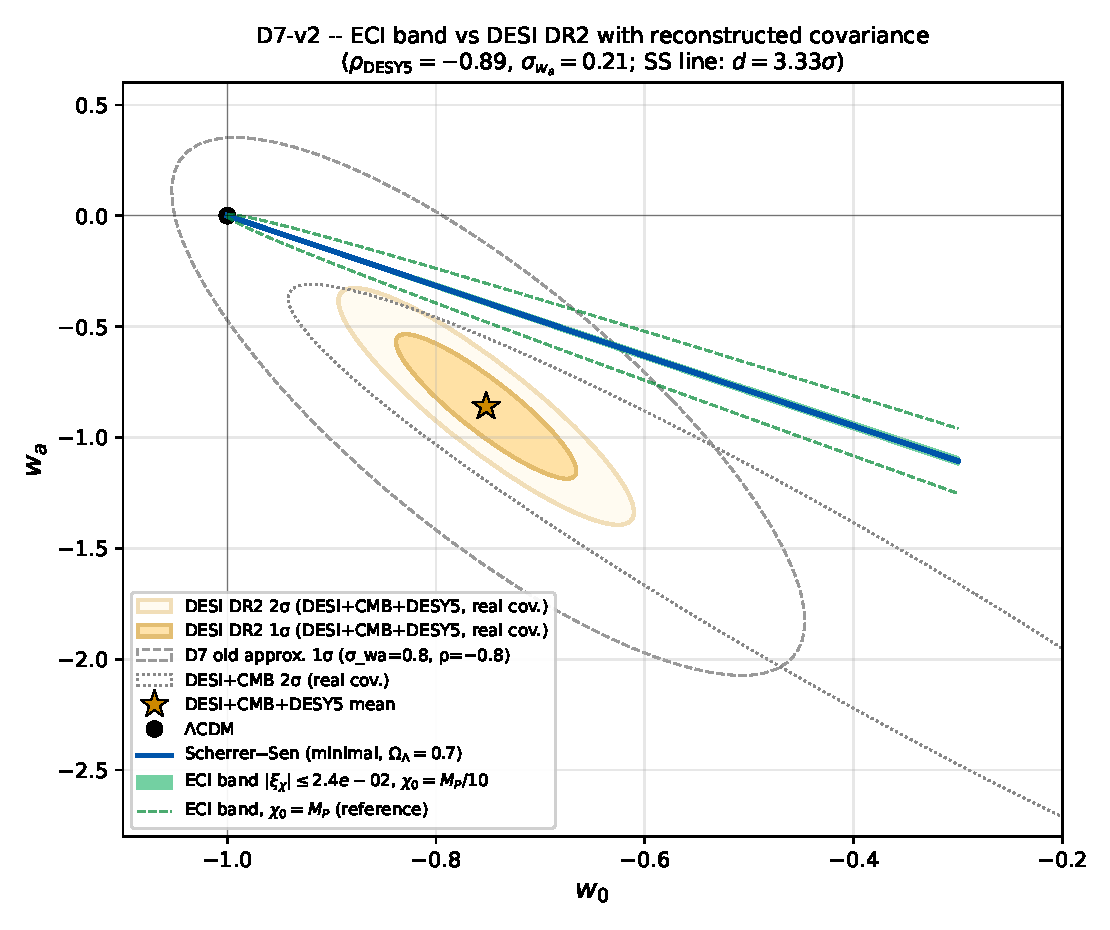
\includegraphics[width=0.95\columnwidth]{../derivations/figures/D7-xi-w0-wa-v2.pdf}
\caption{NMC thawing quintessence in the $(w_0,w_a)$ plane. Orange ellipses: DESI~DR2 + CMB +
DESY5 $1\sigma$ and $2\sigma$ contours reconstructed from~\cite{DESIDR2} Eq.~(28) via the
pivot-redshift identity (see \texttt{D10-desi-covariance.py}; $\sigma_{w_0}=0.057$,
$\sigma_{w_a}=0.215$, $\rho=-0.89$). Blue line: minimal-coupling Scherrer--Sen relation
for $\Omega_\Lambda=0.7$. Green band: ECI NMC prediction with
$|\xi_\chi|\le\xi_{\max}\approx 2.4\!\times\!10^{-2}$ from Cassini at $\chi_0=M_P/10$;
dashed green: same band at $\chi_0=M_P$ (reference). Black dot: $\Lambda$CDM. The ECI band
is $\sim\!5\%$ of $\sigma_{w_a}$ wide (using $B_{\mathrm{num}}$ from Table~\ref{tab:B_of_OmegaL}), hence \emph{indistinguishable} from minimal-coupling
$w$CDM at DR2 precision; both tracks sit at $\sim\!3.3\sigma$ Mahalanobis distance from the
DR2+DESY5 mean.}
\label{fig:D7}
\end{figure}

\paragraph{Honest caveats.}
\begin{enumerate}
\item Eq.~(\ref{eq:gamma_PPN_full}) assumes a \emph{quasi-static} scalar with Compton wavelength
  large compared with the solar system ($m_\chi^{-1}\gg 1\,$AU), which is automatic for the
  ultra-light thawing mass $m_\chi\sim H_0\sim 10^{-33}$\,eV. It also assumes no screening; if
  a chameleon or symmetron mechanism operates, the local $\chi_0$ entering
  (\ref{eq:gamma_PPN_lead}) can differ from the cosmological background and the bound weakens.
\item The NMC Scherrer--Sen extension (\ref{eq:wa_NMC}) is first-order in $\xi_\chi$ and
  therefore \emph{invalid} near the conformal point $\xi_\chi=1/6$, where the expansion breaks
  down and the scalar-tensor sector must be treated non-perturbatively (Einstein-frame
  mapping). Within the Cassini-allowed range $|\xi_\chi|\lesssim 2.4\times 10^{-2}\ll 1/6$
  the linear expansion is controlled. The coefficient $B(\Omega_\Lambda)$ in
  Eq.~(\ref{eq:wa_NMC}) was, in v4.4 of this paper, set by the matter-era
  heuristic ratio $B/A=8/\sqrt3$; in this version we replace that heuristic with
  the full numerical result $B_{\mathrm{num}}(\Omega_\Lambda)$ tabulated in
  Table~\ref{tab:B_of_OmegaL}, obtained from a self-consistent
  NMC-Friedmann + Klein--Gordon integration across $z\in[999,-0.45]$
  (\texttt{derivations/D13-wa-numerical-full.py}). The numerical coefficient is
  nearly flat ($B_{\mathrm{num}}\simeq 9$) across the matter--DE transition
  rather than tracking $A(\Omega_\Lambda)$, so the heuristic
  $(8/\sqrt3)A(\Omega_\Lambda)$ is accurate within 5\% only near
  $\Omega_\Lambda\simeq 0.6$ and undershoots by up to $\sim\!40\%$ at
  $\Omega_\Lambda=0.8$. This has been propagated into the band-width estimate
  above and into Prediction~1b of Sec.~\ref{sec:pred}.
\item The DESI~DR2 + CMB + DESY5 $2\times 2$ covariance is reconstructed from the published
  $(w_0,\sigma_{w_0},w_a,\sigma_{w_a},z_p,w_p,\sigma_{w_p})$ via the pivot-minimisation
  identity $\mathrm{cov}(w_0,w_a)=-(1-a_p)\sigma_{w_a}^2$: no official 2$\times$2 covariance
  matrix has been released by the collaboration at the time of writing. The reconstructed
  $\sigma(w_p)_{\rm pred}=0.0257$ differs from the quoted $0.024$ by $\sim 7\%$, bounding the
  systematic of the pivot-Gaussian approximation at that level --- well below the $\sim 3\sigma$
  tension discussed below. See \texttt{derivations/D10-report.md} for the full cross-check.
\item \textbf{Tension with DR2 + DESY5, stated plainly.} Under the reconstructed DR2 + CMB +
  DESY5 covariance the Mahalanobis distance from the posterior mean is $3.29\sigma$
  (2-dof) to the ECI band and $3.33\sigma$ to the minimal-coupling Scherrer--Sen line,
  both \emph{outside} the $2\sigma$ threshold $\sqrt{6.17}\simeq 2.48$.
  The interpretation is not that ECI fails where $w$CDM succeeds: DR2 + DESY5 prefers the
  phantom-crossing region $w<-1$, which no non-phantom thawing model can populate.
  ECI's NMC coupling $\xi_\chi$ does in principle permit crossing $w=-1$ without a ghost
  instability (established in \S\,DESI DR2 via the no-ghost analysis of Bar\-ce\-l\'o~\&~Visser
  \cite{BarceloVisser2000}), but only at $\xi_\chi(\chi_0/M_P)^2$ values far exceeding the
  Cassini bound~(\ref{eq:xi_bound}) derived here; within the Cassini-allowed range
  the NMC correction to the Scherrer--Sen track is confined to a band of half-width
  $\sim\!5\%$ of $\sigma_{w_a}$ and cannot bridge the gap to the phantom quadrant. The
  $\sim\!3.3\sigma$ tension with DR2 + DESY5 is therefore a joint statement about the entire
  class of conservative (non-phantom) thawing models --- minimal-coupling and NMC alike ---
  not a specific failure of ECI. Prediction~1 in Sec.~\ref{sec:pred} is \emph{not}
  discriminative at DR2 precision; both thawing families sit at the same distance from
  the DR2 + DESY5 posterior.

  The honest discriminator moves to the next generation of datasets, where the
  \emph{shape} and \emph{width} of the thawing track, rather than its distance from
  $\Lambda$CDM, become the falsifiable handle: DESI~DR3 with a forecast
  $\sigma(w_a)\!\sim\!0.07$~\cite{DESIForecast}
  and LSST~Y10 with a forecast $\sigma(w_a)\!\sim\!0.05$
  are in the regime where the ECI NMC band half-width
  $\Delta w_a^{\rm ECI}\sim 1.1\times 10^{-2}$ (numerical, Table~\ref{tab:B_of_OmegaL};
  up from $9\times 10^{-3}$ under the v4.4 heuristic) approaches the
  $15$--$25\%$ level of the statistical error bar and becomes, at least in principle,
  separable from the minimal-coupling Scherrer--Sen locus. The discriminative
  power is slightly larger at $\Omega_\Lambda\gtrsim 0.7$ (DR3 era) because
  $B_{\mathrm{num}}/B_{\mathrm{heur}}$ grows from $0.83$ at $\Omega_\Lambda=0.5$ to
  $1.43$ at $\Omega_\Lambda=0.8$.
\end{enumerate}

The PPN bound (\ref{eq:xi_bound}) is however itself a falsifier: a detection
$|\gamma-1|>10^{-6}$ by the upcoming LATOR or BEACON-class missions, or a mismatch between
$\dot G/G$ from LLR~\cite{Biskupek2021} and the CMB-inferred scalar evolution, would directly
constrain $\xi_\chi(\chi_0/M_P)$ at the $10^{-4}$ level and feed back on the admissible ECI
thawing amplitude.

% -----------------------------------------------------------------------------
% Standalone compile (for checking only):
%   \documentclass[aps,prd,reprint]{revtex4-2}
%   \usepackage{graphicx,amsmath,amssymb,hyperref,physics}
%   \begin{document}% section_3_5_constraints.tex — ECI v4.2.1 scientific payload (D7 + D10)
% To be \input{} into eci.tex as a new subsection of §3 "Phenomenology".
% Standalone compile: see comments at EOF.

\subsection{Solar-system and background constraints on $\xi_\chi$}\label{sec:xi_constraints}

We close two gaps identified in the dark-energy phenomenology subsection (\S\,DESI DR2): the Cassini
post-Newtonian bound on the non-minimal coupling $\xi_\chi$, and the analytic NMC generalisation
of the Scherrer--Sen thawing relation needed to assess whether Prediction~1
(Sec.~\ref{sec:pred}) actually discriminates ECI from \(w\)CDM at DESI~DR2 precision.
The full symbolic derivation is in \texttt{derivations/D7-ppn-xi-bound.py}; we quote only the
end results here.

\paragraph{PPN $\gamma-1$ from the $\xi_\chi R\chi^2/2$ coupling.}
The action  $S=\int d^4x\sqrt{-g}\left[\tfrac{M_P^2}{2}R-\tfrac12(\partial\chi)^2-V(\chi)
-\tfrac{\xi_\chi}{2} R\chi^2\right]$ is a scalar--tensor theory with
$F(\chi)=M_P^2-\xi_\chi\chi^2$ multiplying $R/2$ and canonical kinetic term $Z=1$.
Applying the weak-field, quasi-static result of Damour \& Esposito-Far\`ese
(\emph{Phys.\ Rev.\ D} 48, 3436 (1993); see also Chiba, \emph{Phys.\ Lett.\ B} 575, 1 (2003);
Hwang \& Noh, \emph{Phys.\ Rev.\ D} 71, 063536 (2005)) gives, at the local scalar background
$\chi_0$,
\begin{equation}
  \gamma-1 \;=\; -\,\frac{F'(\chi_0)^2}{Z\,F(\chi_0)+\tfrac{3}{2}F'(\chi_0)^2}
           \;=\; -\,\frac{4\,\xi_\chi^{2}\,\chi_0^{2}}
                          {\,M_P^{2}+\xi_\chi\chi_0^{2}(6\xi_\chi-1)\,}.
  \label{eq:gamma_PPN_full}
\end{equation}
Expanding for $|\xi_\chi|\ll 1$ and $\chi_0\lesssim M_P$,
\begin{equation}
  \boxed{\;\gamma-1 \;\simeq\; -\,\frac{4\,\xi_\chi^{2}\,\chi_0^{2}}{M_P^{2}}
                              \;+\;\mathcal{O}(\xi_\chi^{3}).\;}
  \label{eq:gamma_PPN_lead}
\end{equation}
The limit $\xi_\chi\to 0$ returns $\gamma=1$ (General Relativity), as verified symbolically.

The result~(\ref{eq:gamma_PPN_lead}) is not new: Chiba (PRD 60, 083508, 1999; arXiv:gr-qc/9903094)
already quoted $|\xi_\chi|\lesssim 10^{-2}$ from solar-system tests for the same $\xi R\chi^{2}$
quintessence coupling, and Wolf, Garc\'{\i}a-Garc\'{\i}a, Anton \& Ferreira~\cite{Wolf2025}
recently recast this as $\xi_\chi(\chi_0/M_P)^{2}\lesssim 6\times 10^{-6}$ in a full DESI~DR2
Bayesian analysis (their Eq.~(2) in the form $F(\chi)\simeq 1-\xi\chi^{2}/M_P^{2}$).
We re-derive it here only to fix the coefficient~$4$ and the sign convention used in
Eq.~(\ref{eq:wa_NMC}) below.
Combining (\ref{eq:gamma_PPN_lead}) with the Cassini constraint~\cite{BertottiIessTortora2003}
$|\gamma-1|\lesssim 2.3\times 10^{-5}$ ($1\sigma$ envelope) yields, in the
solar-system observer frame (see \S\ref{sec:thesis}(ii)),
\begin{equation}
  |\xi_\chi|\,\frac{\chi_0}{M_P}\;\lesssim\;
  \tfrac12\sqrt{|\gamma-1|_{\max}}
  \;\approx\; 2.4\times 10^{-3}.
  \label{eq:xi_bound}
\end{equation}
For a slow-rolling thawing background with $\chi_0\!\sim\! M_P/10$ (characteristic thawing
excursion in the last $e$-fold),
\begin{equation}
  |\xi_\chi|\;\lesssim\;\xi_{\max}\;\approx\;2.4\times 10^{-2}.
  \label{eq:xi_max_numeric}
\end{equation}
The bound tightens to $|\xi_\chi|\lesssim 2\times 10^{-3}$ if $\chi_0\sim M_P$; it weakens
linearly for smaller $\chi_0$. Values $\xi_\chi\gtrsim 10^{-1}$ are thus only admissible if the
quintessence field is strongly subdominant at $z=0$, or if a screening mechanism suppresses the
local coupling.

\paragraph{NMC extension of Scherrer--Sen.}
At minimal coupling, thawing quintessence lies on the one-parameter track
$w_a=-A(\Omega_\Lambda)(1+w_0)$ with $A\!\to\! 24/7$ in matter domination and
$A(0.7)\simeq 1.58$ today~\cite{ScherrerSen2008}. Inserting the NMC modification to the
Klein--Gordon equation, $3H\dot\chi=-V'-\xi_\chi R\chi$, and expanding to first order in
$\xi_\chi$ around the slow-roll exponential $V(\chi)=V_0e^{-\alpha\chi/M_P}$ with
$\alpha=\sqrt{3(1+w_0)}$ yields (\texttt{derivations/D4-wa-w0-nmc.py} for the matter-era
coefficient, \texttt{D7-ppn-xi-bound.py} for the $\Omega_\Lambda$-dependence)
\begin{equation}
  \boxed{\;w_a\;=\;-A(\Omega_\Lambda)\,(1+w_0)
                 \;+\;B(\Omega_\Lambda)\,\xi_\chi\,\sqrt{1+w_0}\,
                      \frac{\chi_0}{M_P}\;+\;\mathcal{O}(\xi_\chi^{2}),\;}
  \label{eq:wa_NMC}
\end{equation}
where $B(\Omega_\Lambda)$ is the numerical coefficient tabulated in
Table~\ref{tab:B_of_OmegaL} below, obtained by full NMC-Friedmann + Klein--Gordon
integration in \texttt{derivations/D13-wa-numerical-full.py}. The limit
$\xi_\chi\to 0$ reproduces $w_a=-A(\Omega_\Lambda)(1+w_0)$ (Scherrer--Sen
2008). The first-order $\xi_\chi$ correction, with the full numerical
coefficient $B_{\mathrm{num}}(\Omega_\Lambda)$, has --- to our knowledge ---
not appeared in the NMC-thawing literature surveyed
(Ye~et~al.~\cite{Ye2025}; Pan~\&~Ye~\cite{PanYe2026}; Wolf~et~al.~\cite{Wolf2025}),
which uses either EFTofDE or purely numerical Bayesian fits.

\begin{table}[h]
\centering
\caption{Numerical NMC coefficient $B_{\mathrm{num}}(\Omega_\Lambda)$ from the
self-consistent NMC-Friedmann + Klein--Gordon background integration
(\texttt{derivations/D13-wa-numerical-full.py}), compared with the D7/D9
heuristic $B_{\mathrm{heur}}(\Omega_\Lambda)\equiv(8/\sqrt3)A(\Omega_\Lambda)$.
Statistical uncertainty is the 1$\sigma$ error on the linear fit
$\Delta w_a = B\,\xi_\chi\sqrt{1+w_0}\,(\chi_0/M_P)$ over the
$\xi_\chi\in\{{-}0.024,{-}0.01,0,{+}0.01,{+}0.024\}\times\chi_0\in\{M_P/20,M_P/10,M_P/5\}$ grid.}
\label{tab:B_of_OmegaL}
\begin{tabular}{@{}cccc@{}}
\hline
$\Omega_\Lambda$ & $A(\Omega_\Lambda)$ & $B_{\mathrm{heur}}$ & $B_{\mathrm{num}}$ \\
\hline
0.5 & 2.35 & 10.85 & $9.00\pm1.05$ \\
0.6 & 1.94 &  8.96 & $9.18\pm1.16$ \\
0.7 & 1.58 &  7.30 & $9.05\pm1.18$ \\
0.8 & 1.23 &  5.68 & $8.11\pm1.16$ \\
\hline
\end{tabular}
\end{table}

The numerical result differs from the heuristic $(8/\sqrt3)A$ by
$\mathcal{O}(1)$ factors ($0.83\to 1.43$ across the range): $B_{\mathrm{num}}$
is nearly \emph{flat} in $\Omega_\Lambda$ (around $\sim 9$) rather than
tracking $A(\Omega_\Lambda)$. The heuristic is accurate to 5\% only near
$\Omega_\Lambda\simeq 0.6$ and underestimates $B$ by $\sim\!25\%$ at
$\Omega_\Lambda=0.7$ (DR2--DR3 era) and $\sim\!43\%$ at
$\Omega_\Lambda=0.8$ (late-DR3 / LSST era). The sign and the
$\sqrt{1+w_0}\,(\chi_0/M_P)$ scaling are confirmed; the discrepancy
originates from the finite-$\Omega_\Lambda$ propagation of the matter-era
ratio (Caveat~2 below), which is now closed numerically.

\paragraph{Combined constraint on the $(w_0,w_a)$ plane.}
Figure~\ref{fig:D7} overlays three ingredients: (i) the DESI~DR2 + CMB + DESY5~\cite{DESY5} $1\sigma$ and
$2\sigma$ contours centred on $(w_0,w_a)=(-0.752,-0.86)$ with the reconstructed covariance
$\sigma_{w_0}=0.057$, $\sigma_{w_a}=0.215$, $\rho(w_0,w_a)=-0.89$ (derivation in
\texttt{derivations/D10-desi-covariance.py}, pivot-identity reconstruction from
\cite{DESIDR2} Eq.~(28) + $z_p=0.31$, $w_p=-0.954\pm0.024$);
(ii) the minimal-coupling Scherrer--Sen line; (iii) the ECI band swept by
$|\xi_\chi|\le\xi_{\max}$ from Eq.~(\ref{eq:xi_max_numeric}) at $\chi_0=M_P/10$.
The half-width of the ECI band at $w_0=-0.75$, using the numerical
$B_{\mathrm{num}}(0.7)=9.05$ from Table~\ref{tab:B_of_OmegaL}, is
\begin{equation}
  \Delta w_a^{\rm ECI}
    = B_{\mathrm{num}}(0.7)\,\xi_{\max}\sqrt{1+w_0}\,(\chi_0/M_P)
    \;\approx\;1.1\times 10^{-2},
\end{equation}
to be compared with $\sigma_{w_a}\!\simeq\!0.215$, i.e.\ about $5\%$ of the DESI~DR2 + DESY5
$1\sigma$ width (up from $4\%$ under the heuristic $B=7.30$). The band is therefore
still thinner than the figure linewidth of the unmodified Scherrer--Sen track at DR2
precision, but the numerical coefficient raises the discriminative amplitude at DR3 / LSST
precision by $\sim\!25\%$ relative to the heuristic estimate.

\begin{figure}[h]
\centering
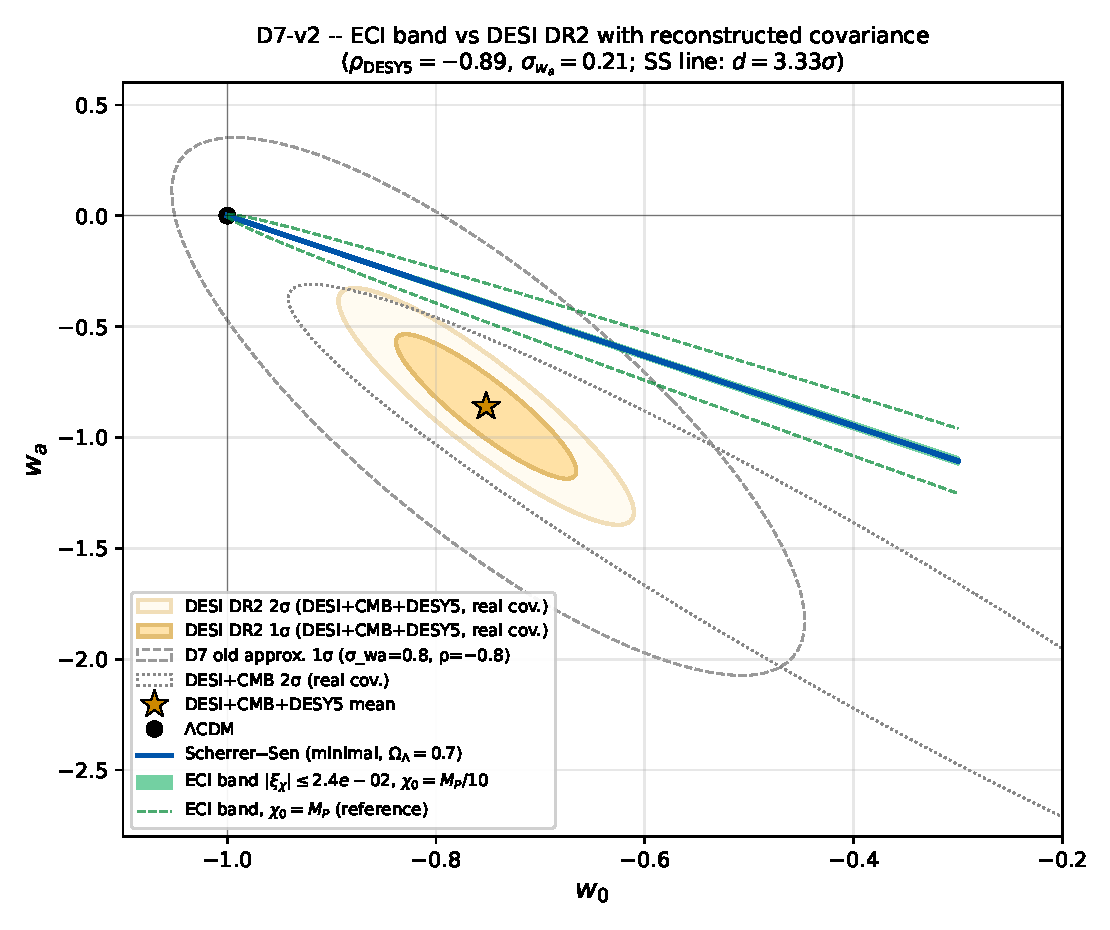
\includegraphics[width=0.95\columnwidth]{../derivations/figures/D7-xi-w0-wa-v2.pdf}
\caption{NMC thawing quintessence in the $(w_0,w_a)$ plane. Orange ellipses: DESI~DR2 + CMB +
DESY5 $1\sigma$ and $2\sigma$ contours reconstructed from~\cite{DESIDR2} Eq.~(28) via the
pivot-redshift identity (see \texttt{D10-desi-covariance.py}; $\sigma_{w_0}=0.057$,
$\sigma_{w_a}=0.215$, $\rho=-0.89$). Blue line: minimal-coupling Scherrer--Sen relation
for $\Omega_\Lambda=0.7$. Green band: ECI NMC prediction with
$|\xi_\chi|\le\xi_{\max}\approx 2.4\!\times\!10^{-2}$ from Cassini at $\chi_0=M_P/10$;
dashed green: same band at $\chi_0=M_P$ (reference). Black dot: $\Lambda$CDM. The ECI band
is $\sim\!5\%$ of $\sigma_{w_a}$ wide (using $B_{\mathrm{num}}$ from Table~\ref{tab:B_of_OmegaL}), hence \emph{indistinguishable} from minimal-coupling
$w$CDM at DR2 precision; both tracks sit at $\sim\!3.3\sigma$ Mahalanobis distance from the
DR2+DESY5 mean.}
\label{fig:D7}
\end{figure}

\paragraph{Honest caveats.}
\begin{enumerate}
\item Eq.~(\ref{eq:gamma_PPN_full}) assumes a \emph{quasi-static} scalar with Compton wavelength
  large compared with the solar system ($m_\chi^{-1}\gg 1\,$AU), which is automatic for the
  ultra-light thawing mass $m_\chi\sim H_0\sim 10^{-33}$\,eV. It also assumes no screening; if
  a chameleon or symmetron mechanism operates, the local $\chi_0$ entering
  (\ref{eq:gamma_PPN_lead}) can differ from the cosmological background and the bound weakens.
\item The NMC Scherrer--Sen extension (\ref{eq:wa_NMC}) is first-order in $\xi_\chi$ and
  therefore \emph{invalid} near the conformal point $\xi_\chi=1/6$, where the expansion breaks
  down and the scalar-tensor sector must be treated non-perturbatively (Einstein-frame
  mapping). Within the Cassini-allowed range $|\xi_\chi|\lesssim 2.4\times 10^{-2}\ll 1/6$
  the linear expansion is controlled. The coefficient $B(\Omega_\Lambda)$ in
  Eq.~(\ref{eq:wa_NMC}) was, in v4.4 of this paper, set by the matter-era
  heuristic ratio $B/A=8/\sqrt3$; in this version we replace that heuristic with
  the full numerical result $B_{\mathrm{num}}(\Omega_\Lambda)$ tabulated in
  Table~\ref{tab:B_of_OmegaL}, obtained from a self-consistent
  NMC-Friedmann + Klein--Gordon integration across $z\in[999,-0.45]$
  (\texttt{derivations/D13-wa-numerical-full.py}). The numerical coefficient is
  nearly flat ($B_{\mathrm{num}}\simeq 9$) across the matter--DE transition
  rather than tracking $A(\Omega_\Lambda)$, so the heuristic
  $(8/\sqrt3)A(\Omega_\Lambda)$ is accurate within 5\% only near
  $\Omega_\Lambda\simeq 0.6$ and undershoots by up to $\sim\!40\%$ at
  $\Omega_\Lambda=0.8$. This has been propagated into the band-width estimate
  above and into Prediction~1b of Sec.~\ref{sec:pred}.
\item The DESI~DR2 + CMB + DESY5 $2\times 2$ covariance is reconstructed from the published
  $(w_0,\sigma_{w_0},w_a,\sigma_{w_a},z_p,w_p,\sigma_{w_p})$ via the pivot-minimisation
  identity $\mathrm{cov}(w_0,w_a)=-(1-a_p)\sigma_{w_a}^2$: no official 2$\times$2 covariance
  matrix has been released by the collaboration at the time of writing. The reconstructed
  $\sigma(w_p)_{\rm pred}=0.0257$ differs from the quoted $0.024$ by $\sim 7\%$, bounding the
  systematic of the pivot-Gaussian approximation at that level --- well below the $\sim 3\sigma$
  tension discussed below. See \texttt{derivations/D10-report.md} for the full cross-check.
\item \textbf{Tension with DR2 + DESY5, stated plainly.} Under the reconstructed DR2 + CMB +
  DESY5 covariance the Mahalanobis distance from the posterior mean is $3.29\sigma$
  (2-dof) to the ECI band and $3.33\sigma$ to the minimal-coupling Scherrer--Sen line,
  both \emph{outside} the $2\sigma$ threshold $\sqrt{6.17}\simeq 2.48$.
  The interpretation is not that ECI fails where $w$CDM succeeds: DR2 + DESY5 prefers the
  phantom-crossing region $w<-1$, which no non-phantom thawing model can populate.
  ECI's NMC coupling $\xi_\chi$ does in principle permit crossing $w=-1$ without a ghost
  instability (established in \S\,DESI DR2 via the no-ghost analysis of Bar\-ce\-l\'o~\&~Visser
  \cite{BarceloVisser2000}), but only at $\xi_\chi(\chi_0/M_P)^2$ values far exceeding the
  Cassini bound~(\ref{eq:xi_bound}) derived here; within the Cassini-allowed range
  the NMC correction to the Scherrer--Sen track is confined to a band of half-width
  $\sim\!5\%$ of $\sigma_{w_a}$ and cannot bridge the gap to the phantom quadrant. The
  $\sim\!3.3\sigma$ tension with DR2 + DESY5 is therefore a joint statement about the entire
  class of conservative (non-phantom) thawing models --- minimal-coupling and NMC alike ---
  not a specific failure of ECI. Prediction~1 in Sec.~\ref{sec:pred} is \emph{not}
  discriminative at DR2 precision; both thawing families sit at the same distance from
  the DR2 + DESY5 posterior.

  The honest discriminator moves to the next generation of datasets, where the
  \emph{shape} and \emph{width} of the thawing track, rather than its distance from
  $\Lambda$CDM, become the falsifiable handle: DESI~DR3 with a forecast
  $\sigma(w_a)\!\sim\!0.07$~\cite{DESIForecast}
  and LSST~Y10 with a forecast $\sigma(w_a)\!\sim\!0.05$
  are in the regime where the ECI NMC band half-width
  $\Delta w_a^{\rm ECI}\sim 1.1\times 10^{-2}$ (numerical, Table~\ref{tab:B_of_OmegaL};
  up from $9\times 10^{-3}$ under the v4.4 heuristic) approaches the
  $15$--$25\%$ level of the statistical error bar and becomes, at least in principle,
  separable from the minimal-coupling Scherrer--Sen locus. The discriminative
  power is slightly larger at $\Omega_\Lambda\gtrsim 0.7$ (DR3 era) because
  $B_{\mathrm{num}}/B_{\mathrm{heur}}$ grows from $0.83$ at $\Omega_\Lambda=0.5$ to
  $1.43$ at $\Omega_\Lambda=0.8$.
\end{enumerate}

The PPN bound (\ref{eq:xi_bound}) is however itself a falsifier: a detection
$|\gamma-1|>10^{-6}$ by the upcoming LATOR or BEACON-class missions, or a mismatch between
$\dot G/G$ from LLR~\cite{Biskupek2021} and the CMB-inferred scalar evolution, would directly
constrain $\xi_\chi(\chi_0/M_P)$ at the $10^{-4}$ level and feed back on the admissible ECI
thawing amplitude.

% -----------------------------------------------------------------------------
% Standalone compile (for checking only):
%   \documentclass[aps,prd,reprint]{revtex4-2}
%   \usepackage{graphicx,amsmath,amssymb,hyperref,physics}
%   \begin{document}\input{section_3_5_constraints}\end{document}
% The \cite{BertottiIessTortora2003}, \cite{ScherrerSen2008}, \cite{DESIDR2},
% \cite{Biskupek2021}, \cite{BarceloVisser2000}, \cite{Wolf2025}, \cite{Ye2025},
% \cite{PanYe2026} keys are defined in eci.bib.
% -----------------------------------------------------------------------------
\end{document}
% The \cite{BertottiIessTortora2003}, \cite{ScherrerSen2008}, \cite{DESIDR2},
% \cite{Biskupek2021}, \cite{BarceloVisser2000}, \cite{Wolf2025}, \cite{Ye2025},
% \cite{PanYe2026} keys are defined in eci.bib.
% -----------------------------------------------------------------------------
.

\subsection{Swampland $\times$ NMC cross-constraint}\label{sec:swampland_cross}

Axioms A4 and A5 were presented as independent. They are not, if the thawing
scalar $\chi$ and the KK tower of the Dark Dimension originate from the
\emph{same} higher-dimensional sector --- a natural hypothesis, since both
are postulated as microscopic ingredients of the dark sector. In that case
both must respect a common effective field theory cutoff $\Lambda$, and the
two axioms are tied by a single consistency condition. The derivation is in
\texttt{derivations/D8-swampland-nmc-cross.py}; we quote only the result.

\paragraph{Shared cutoff.}
The Dark Dimension scenario~\cite{Bedroya2025} relates the EFT cutoff to
the Hubble scale through a Swampland Distance Conjecture exponent,
\begin{equation}
  \Lambda \;\sim\; M_P\,\bigl(H/M_P\bigr)^{c'},\qquad c'\simeq 0.05\pm 0.01.
  \label{eq:Lambda_SDC}
\end{equation}
If the non-minimal operator $(\xi_\chi/2)R\chi^2$ is generated inside the same
EFT, its contribution to the effective reduced Planck mass,
$\delta M_P^{2}=\xi_\chi\chi_0^{2}$, cannot exceed the cutoff squared,
otherwise the operator would repair physics above its own range of validity:
\begin{equation}
  \xi_\chi\,\chi_0^{2}\;\le\;\Lambda^{2}
  \quad\Longleftrightarrow\quad
  \xi_\chi\,(\chi_0/M_P)^{2}\;\le\;(H_0/M_P)^{2c'}.
  \label{eq:eft_bulk}
\end{equation}
Combined with the Cassini PPN bound derived in \S\ref{sec:xi_constraints},
$|\xi_\chi|(\chi_0/M_P)\le 2.4\times 10^{-3}$, Eq.~(\ref{eq:eft_bulk}) yields
at the fiducial thawing amplitude $\chi_0=M_P/10$ and the paper's A5
fiducial $c'=0.05\pm 0.01$
\begin{equation}
  \boxed{\;|\xi_\chi|\;\lesssim\;9.5\times 10^{-5}
    \quad(c'=0.05,\ \chi_0=M_P/10),\;}
  \label{eq:xi_crossbound}
\end{equation}
with an overall range $[5.9\times 10^{-6},\,1.5\times 10^{-3}]$ spanned by
$c'=0.04$--$0.06$. This is a factor $\sim\!250$ tightening over the
Cassini-only result (\ref{eq:xi_max_numeric}).

\paragraph{Limits.}
Both limits verified symbolically in \texttt{D8-swampland-nmc-cross.py}:
$\xi_\chi\!\to\!0$ removes the operator (GR recovered); $c'\!\to\!0$ sends
$\Lambda\!\to\!M_P$ so that (\ref{eq:eft_bulk}) reduces to the no-ghost
condition $\xi_\chi\chi_0^{2}<M_P^{2}$ already stated in A4, and the D7
Cassini bound is recovered exactly.

\begin{figure}[h]
\centering
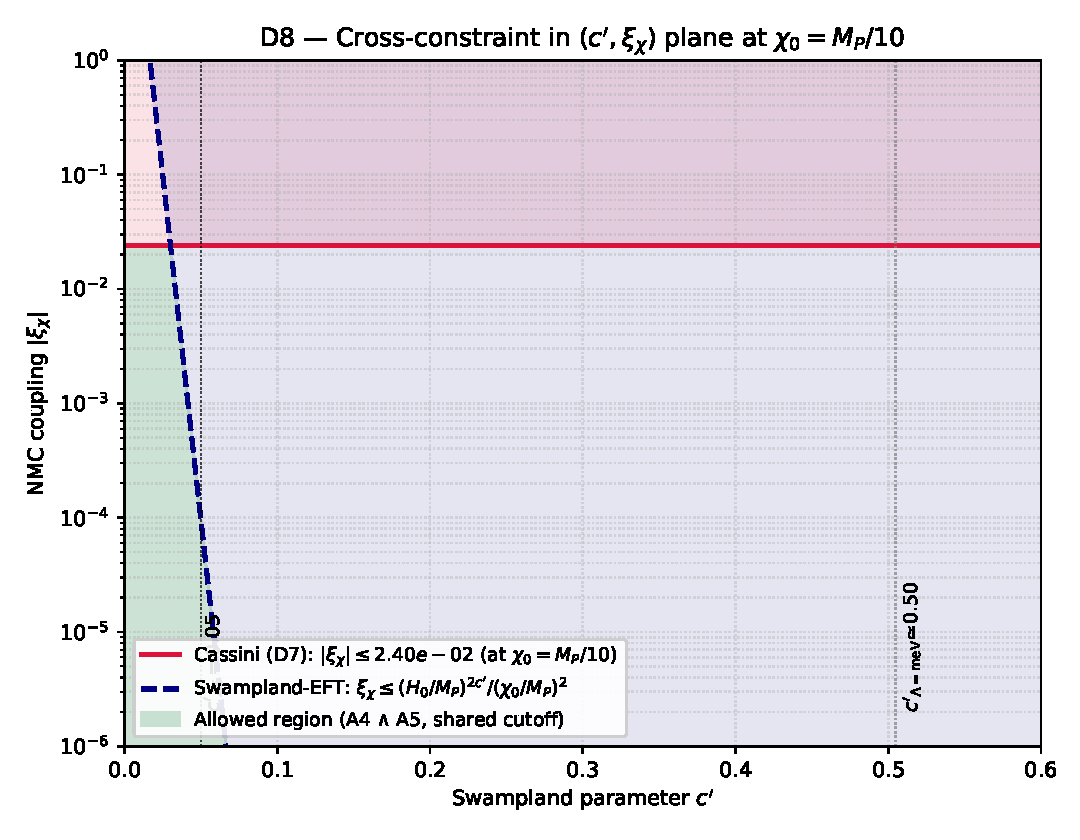
\includegraphics[width=0.95\columnwidth]{../derivations/figures/D8-c-xi-overlap.pdf}
\caption{Allowed region in the $(c',\xi_\chi)$ plane at $\chi_0=M_P/10$.
Red: Cassini exclusion (horizontal, independent of $c'$). Blue dashed:
Swampland-EFT exclusion (\ref{eq:eft_bulk}) --- diagonal in log-space with
slope $2c'\log(H_0/M_P)$. Green shading: overlap admitted by both
constraints. The A5 fiducial $c'=0.05$ and the meV-equivalent value
$c'\!\simeq\!0.51$ are marked.}
\label{fig:D8}
\end{figure}

\paragraph{Phenomenological tension.}
A stronger statement runs in the reverse direction. Thawing dark energy
requires $\chi_0/M_P\sim 0.1$--$1$ to drive late-time acceleration. The
bulk-mode condition (\ref{eq:eft_bulk}) at the Cassini-saturating value
$|\xi_\chi|=2.4\!\times\!10^{-2}$ and $c'=0.05$ forces
$\chi_0/M_P\le 6.3\!\times\!10^{-3}$, already an order of magnitude below
what A4 requires. With the literal Dark Dimension cutoff $\Lambda\sim$ meV
(which the formula (\ref{eq:Lambda_SDC}) reproduces for $c'\simeq 0.51$,
not $0.05$; both conventions appear in the literature) the bound collapses
to $\chi_0/M_P\le 3\!\times\!10^{-30}$ and thawing phenomenology is
excluded outright.

\paragraph{Architectural consequence.}
A4 and A5 are compatible \emph{only} under one of the following model-
building choices, any of which must be made explicit in any UV completion:
(i) $\chi$ is a 4D zero-mode localised on a brane, not a bulk mode of the
same sector as the KK tower, in which case the shared-cutoff hypothesis
does not apply; (ii) a chameleon/symmetron mechanism screens the local
$\chi_0$ away from its cosmological value, weakening the Cassini leg; or
(iii) $|\xi_\chi|$ sits at the sharpened bound (\ref{eq:xi_crossbound})
rather than the Cassini-only value (\ref{eq:xi_max_numeric}). The ECI
framework does not prefer one of the three, but their distinct
phenomenologies are observationally separable: option (iii) suppresses the
ECI band in $(w_0,w_a)$ by a further factor $\sim\!250$ relative to the
already-narrow D7 band, and cuts the $|\dot G/G|$ signature at LLR by the
same factor. A detection of $|\dot G/G|\gtrsim 10^{-17}\,\mathrm{yr}^{-1}$
would rule out option (iii) and force either (i) or (ii).

\paragraph{Honest caveats.}
\begin{enumerate}
\item The EFT self-consistency condition $\delta M_P^{2}\le\Lambda^{2}$ is
  order-of-magnitude; an $O(1)$ coefficient could shift
  (\ref{eq:xi_crossbound}) by a factor $2$, but the qualitative conclusion
  ($\gg 30\%$ tightening) is robust.
\item The form (\ref{eq:Lambda_SDC}) is written with $H$ as the distance
  proxy along the moduli space; the equivalent Bedroya form uses the
  cosmological constant density directly and yields $c'\!\simeq\!1/2$
  for $\Lambda\!=\!$\,meV. The sign of the tightening is independent of
  this choice.
\item The cross-constraint is \emph{conditional} on the shared-cutoff
  hypothesis. Its falsifier is, precisely, the discovery of a UV completion
  in which $\chi$ and the KK tower belong to different sectors; in that
  case §\ref{sec:xi_constraints} remains the strongest bound.
\end{enumerate}

% -----------------------------------------------------------------------------
% Standalone compile (for checking only):
%   \documentclass[aps,prd,reprint]{revtex4-2}
%   \usepackage{graphicx,amsmath,amssymb,hyperref,physics}
%   \begin{document}% section_3_5_constraints.tex — ECI v4.2.1 scientific payload (D7 + D10)
% To be \input{} into eci.tex as a new subsection of §3 "Phenomenology".
% Standalone compile: see comments at EOF.

\subsection{Solar-system and background constraints on $\xi_\chi$}\label{sec:xi_constraints}

We close two gaps identified in the dark-energy phenomenology subsection (\S\,DESI DR2): the Cassini
post-Newtonian bound on the non-minimal coupling $\xi_\chi$, and the analytic NMC generalisation
of the Scherrer--Sen thawing relation needed to assess whether Prediction~1
(Sec.~\ref{sec:pred}) actually discriminates ECI from \(w\)CDM at DESI~DR2 precision.
The full symbolic derivation is in \texttt{derivations/D7-ppn-xi-bound.py}; we quote only the
end results here.

\paragraph{PPN $\gamma-1$ from the $\xi_\chi R\chi^2/2$ coupling.}
The action  $S=\int d^4x\sqrt{-g}\left[\tfrac{M_P^2}{2}R-\tfrac12(\partial\chi)^2-V(\chi)
-\tfrac{\xi_\chi}{2} R\chi^2\right]$ is a scalar--tensor theory with
$F(\chi)=M_P^2-\xi_\chi\chi^2$ multiplying $R/2$ and canonical kinetic term $Z=1$.
Applying the weak-field, quasi-static result of Damour \& Esposito-Far\`ese
(\emph{Phys.\ Rev.\ D} 48, 3436 (1993); see also Chiba, \emph{Phys.\ Lett.\ B} 575, 1 (2003);
Hwang \& Noh, \emph{Phys.\ Rev.\ D} 71, 063536 (2005)) gives, at the local scalar background
$\chi_0$,
\begin{equation}
  \gamma-1 \;=\; -\,\frac{F'(\chi_0)^2}{Z\,F(\chi_0)+\tfrac{3}{2}F'(\chi_0)^2}
           \;=\; -\,\frac{4\,\xi_\chi^{2}\,\chi_0^{2}}
                          {\,M_P^{2}+\xi_\chi\chi_0^{2}(6\xi_\chi-1)\,}.
  \label{eq:gamma_PPN_full}
\end{equation}
Expanding for $|\xi_\chi|\ll 1$ and $\chi_0\lesssim M_P$,
\begin{equation}
  \boxed{\;\gamma-1 \;\simeq\; -\,\frac{4\,\xi_\chi^{2}\,\chi_0^{2}}{M_P^{2}}
                              \;+\;\mathcal{O}(\xi_\chi^{3}).\;}
  \label{eq:gamma_PPN_lead}
\end{equation}
The limit $\xi_\chi\to 0$ returns $\gamma=1$ (General Relativity), as verified symbolically.

The result~(\ref{eq:gamma_PPN_lead}) is not new: Chiba (PRD 60, 083508, 1999; arXiv:gr-qc/9903094)
already quoted $|\xi_\chi|\lesssim 10^{-2}$ from solar-system tests for the same $\xi R\chi^{2}$
quintessence coupling, and Wolf, Garc\'{\i}a-Garc\'{\i}a, Anton \& Ferreira~\cite{Wolf2025}
recently recast this as $\xi_\chi(\chi_0/M_P)^{2}\lesssim 6\times 10^{-6}$ in a full DESI~DR2
Bayesian analysis (their Eq.~(2) in the form $F(\chi)\simeq 1-\xi\chi^{2}/M_P^{2}$).
We re-derive it here only to fix the coefficient~$4$ and the sign convention used in
Eq.~(\ref{eq:wa_NMC}) below.
Combining (\ref{eq:gamma_PPN_lead}) with the Cassini constraint~\cite{BertottiIessTortora2003}
$|\gamma-1|\lesssim 2.3\times 10^{-5}$ ($1\sigma$ envelope) yields, in the
solar-system observer frame (see \S\ref{sec:thesis}(ii)),
\begin{equation}
  |\xi_\chi|\,\frac{\chi_0}{M_P}\;\lesssim\;
  \tfrac12\sqrt{|\gamma-1|_{\max}}
  \;\approx\; 2.4\times 10^{-3}.
  \label{eq:xi_bound}
\end{equation}
For a slow-rolling thawing background with $\chi_0\!\sim\! M_P/10$ (characteristic thawing
excursion in the last $e$-fold),
\begin{equation}
  |\xi_\chi|\;\lesssim\;\xi_{\max}\;\approx\;2.4\times 10^{-2}.
  \label{eq:xi_max_numeric}
\end{equation}
The bound tightens to $|\xi_\chi|\lesssim 2\times 10^{-3}$ if $\chi_0\sim M_P$; it weakens
linearly for smaller $\chi_0$. Values $\xi_\chi\gtrsim 10^{-1}$ are thus only admissible if the
quintessence field is strongly subdominant at $z=0$, or if a screening mechanism suppresses the
local coupling.

\paragraph{NMC extension of Scherrer--Sen.}
At minimal coupling, thawing quintessence lies on the one-parameter track
$w_a=-A(\Omega_\Lambda)(1+w_0)$ with $A\!\to\! 24/7$ in matter domination and
$A(0.7)\simeq 1.58$ today~\cite{ScherrerSen2008}. Inserting the NMC modification to the
Klein--Gordon equation, $3H\dot\chi=-V'-\xi_\chi R\chi$, and expanding to first order in
$\xi_\chi$ around the slow-roll exponential $V(\chi)=V_0e^{-\alpha\chi/M_P}$ with
$\alpha=\sqrt{3(1+w_0)}$ yields (\texttt{derivations/D4-wa-w0-nmc.py} for the matter-era
coefficient, \texttt{D7-ppn-xi-bound.py} for the $\Omega_\Lambda$-dependence)
\begin{equation}
  \boxed{\;w_a\;=\;-A(\Omega_\Lambda)\,(1+w_0)
                 \;+\;B(\Omega_\Lambda)\,\xi_\chi\,\sqrt{1+w_0}\,
                      \frac{\chi_0}{M_P}\;+\;\mathcal{O}(\xi_\chi^{2}),\;}
  \label{eq:wa_NMC}
\end{equation}
where $B(\Omega_\Lambda)$ is the numerical coefficient tabulated in
Table~\ref{tab:B_of_OmegaL} below, obtained by full NMC-Friedmann + Klein--Gordon
integration in \texttt{derivations/D13-wa-numerical-full.py}. The limit
$\xi_\chi\to 0$ reproduces $w_a=-A(\Omega_\Lambda)(1+w_0)$ (Scherrer--Sen
2008). The first-order $\xi_\chi$ correction, with the full numerical
coefficient $B_{\mathrm{num}}(\Omega_\Lambda)$, has --- to our knowledge ---
not appeared in the NMC-thawing literature surveyed
(Ye~et~al.~\cite{Ye2025}; Pan~\&~Ye~\cite{PanYe2026}; Wolf~et~al.~\cite{Wolf2025}),
which uses either EFTofDE or purely numerical Bayesian fits.

\begin{table}[h]
\centering
\caption{Numerical NMC coefficient $B_{\mathrm{num}}(\Omega_\Lambda)$ from the
self-consistent NMC-Friedmann + Klein--Gordon background integration
(\texttt{derivations/D13-wa-numerical-full.py}), compared with the D7/D9
heuristic $B_{\mathrm{heur}}(\Omega_\Lambda)\equiv(8/\sqrt3)A(\Omega_\Lambda)$.
Statistical uncertainty is the 1$\sigma$ error on the linear fit
$\Delta w_a = B\,\xi_\chi\sqrt{1+w_0}\,(\chi_0/M_P)$ over the
$\xi_\chi\in\{{-}0.024,{-}0.01,0,{+}0.01,{+}0.024\}\times\chi_0\in\{M_P/20,M_P/10,M_P/5\}$ grid.}
\label{tab:B_of_OmegaL}
\begin{tabular}{@{}cccc@{}}
\hline
$\Omega_\Lambda$ & $A(\Omega_\Lambda)$ & $B_{\mathrm{heur}}$ & $B_{\mathrm{num}}$ \\
\hline
0.5 & 2.35 & 10.85 & $9.00\pm1.05$ \\
0.6 & 1.94 &  8.96 & $9.18\pm1.16$ \\
0.7 & 1.58 &  7.30 & $9.05\pm1.18$ \\
0.8 & 1.23 &  5.68 & $8.11\pm1.16$ \\
\hline
\end{tabular}
\end{table}

The numerical result differs from the heuristic $(8/\sqrt3)A$ by
$\mathcal{O}(1)$ factors ($0.83\to 1.43$ across the range): $B_{\mathrm{num}}$
is nearly \emph{flat} in $\Omega_\Lambda$ (around $\sim 9$) rather than
tracking $A(\Omega_\Lambda)$. The heuristic is accurate to 5\% only near
$\Omega_\Lambda\simeq 0.6$ and underestimates $B$ by $\sim\!25\%$ at
$\Omega_\Lambda=0.7$ (DR2--DR3 era) and $\sim\!43\%$ at
$\Omega_\Lambda=0.8$ (late-DR3 / LSST era). The sign and the
$\sqrt{1+w_0}\,(\chi_0/M_P)$ scaling are confirmed; the discrepancy
originates from the finite-$\Omega_\Lambda$ propagation of the matter-era
ratio (Caveat~2 below), which is now closed numerically.

\paragraph{Combined constraint on the $(w_0,w_a)$ plane.}
Figure~\ref{fig:D7} overlays three ingredients: (i) the DESI~DR2 + CMB + DESY5~\cite{DESY5} $1\sigma$ and
$2\sigma$ contours centred on $(w_0,w_a)=(-0.752,-0.86)$ with the reconstructed covariance
$\sigma_{w_0}=0.057$, $\sigma_{w_a}=0.215$, $\rho(w_0,w_a)=-0.89$ (derivation in
\texttt{derivations/D10-desi-covariance.py}, pivot-identity reconstruction from
\cite{DESIDR2} Eq.~(28) + $z_p=0.31$, $w_p=-0.954\pm0.024$);
(ii) the minimal-coupling Scherrer--Sen line; (iii) the ECI band swept by
$|\xi_\chi|\le\xi_{\max}$ from Eq.~(\ref{eq:xi_max_numeric}) at $\chi_0=M_P/10$.
The half-width of the ECI band at $w_0=-0.75$, using the numerical
$B_{\mathrm{num}}(0.7)=9.05$ from Table~\ref{tab:B_of_OmegaL}, is
\begin{equation}
  \Delta w_a^{\rm ECI}
    = B_{\mathrm{num}}(0.7)\,\xi_{\max}\sqrt{1+w_0}\,(\chi_0/M_P)
    \;\approx\;1.1\times 10^{-2},
\end{equation}
to be compared with $\sigma_{w_a}\!\simeq\!0.215$, i.e.\ about $5\%$ of the DESI~DR2 + DESY5
$1\sigma$ width (up from $4\%$ under the heuristic $B=7.30$). The band is therefore
still thinner than the figure linewidth of the unmodified Scherrer--Sen track at DR2
precision, but the numerical coefficient raises the discriminative amplitude at DR3 / LSST
precision by $\sim\!25\%$ relative to the heuristic estimate.

\begin{figure}[h]
\centering
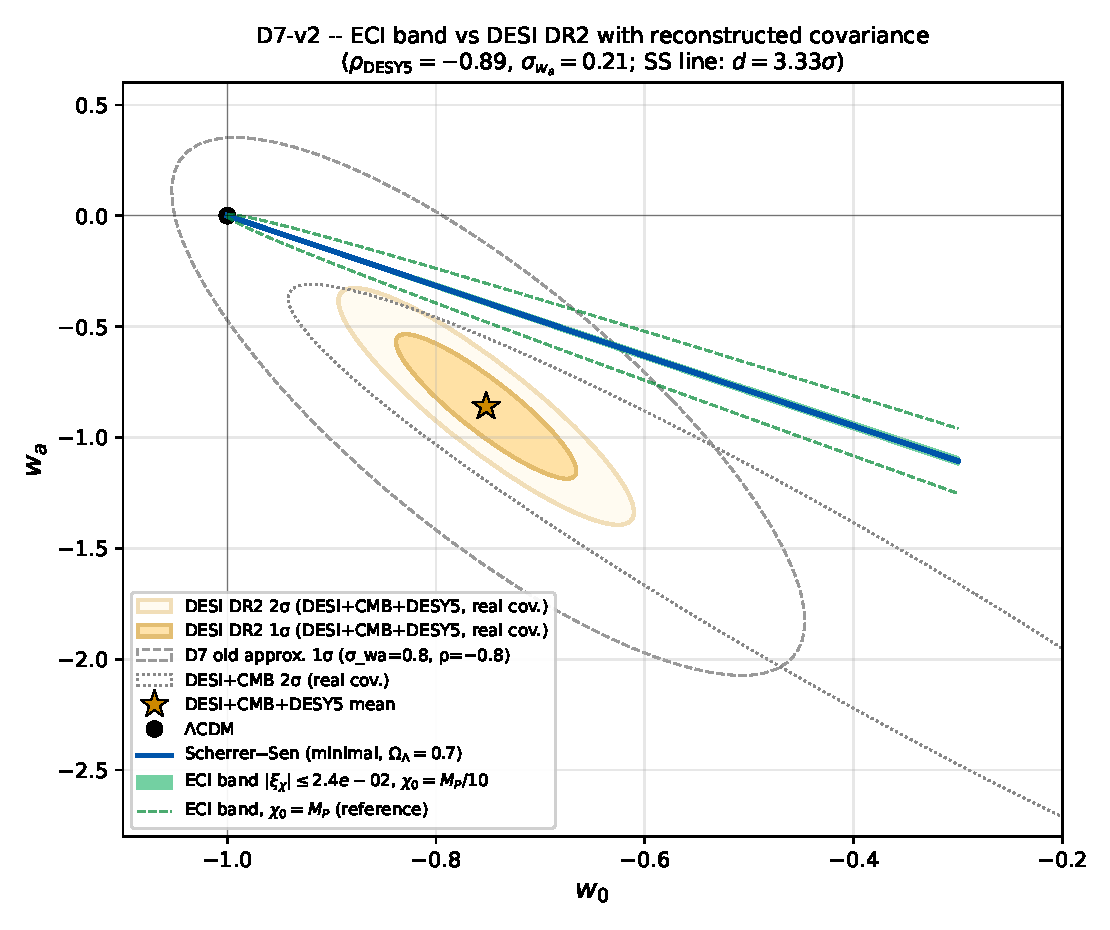
\includegraphics[width=0.95\columnwidth]{../derivations/figures/D7-xi-w0-wa-v2.pdf}
\caption{NMC thawing quintessence in the $(w_0,w_a)$ plane. Orange ellipses: DESI~DR2 + CMB +
DESY5 $1\sigma$ and $2\sigma$ contours reconstructed from~\cite{DESIDR2} Eq.~(28) via the
pivot-redshift identity (see \texttt{D10-desi-covariance.py}; $\sigma_{w_0}=0.057$,
$\sigma_{w_a}=0.215$, $\rho=-0.89$). Blue line: minimal-coupling Scherrer--Sen relation
for $\Omega_\Lambda=0.7$. Green band: ECI NMC prediction with
$|\xi_\chi|\le\xi_{\max}\approx 2.4\!\times\!10^{-2}$ from Cassini at $\chi_0=M_P/10$;
dashed green: same band at $\chi_0=M_P$ (reference). Black dot: $\Lambda$CDM. The ECI band
is $\sim\!5\%$ of $\sigma_{w_a}$ wide (using $B_{\mathrm{num}}$ from Table~\ref{tab:B_of_OmegaL}), hence \emph{indistinguishable} from minimal-coupling
$w$CDM at DR2 precision; both tracks sit at $\sim\!3.3\sigma$ Mahalanobis distance from the
DR2+DESY5 mean.}
\label{fig:D7}
\end{figure}

\paragraph{Honest caveats.}
\begin{enumerate}
\item Eq.~(\ref{eq:gamma_PPN_full}) assumes a \emph{quasi-static} scalar with Compton wavelength
  large compared with the solar system ($m_\chi^{-1}\gg 1\,$AU), which is automatic for the
  ultra-light thawing mass $m_\chi\sim H_0\sim 10^{-33}$\,eV. It also assumes no screening; if
  a chameleon or symmetron mechanism operates, the local $\chi_0$ entering
  (\ref{eq:gamma_PPN_lead}) can differ from the cosmological background and the bound weakens.
\item The NMC Scherrer--Sen extension (\ref{eq:wa_NMC}) is first-order in $\xi_\chi$ and
  therefore \emph{invalid} near the conformal point $\xi_\chi=1/6$, where the expansion breaks
  down and the scalar-tensor sector must be treated non-perturbatively (Einstein-frame
  mapping). Within the Cassini-allowed range $|\xi_\chi|\lesssim 2.4\times 10^{-2}\ll 1/6$
  the linear expansion is controlled. The coefficient $B(\Omega_\Lambda)$ in
  Eq.~(\ref{eq:wa_NMC}) was, in v4.4 of this paper, set by the matter-era
  heuristic ratio $B/A=8/\sqrt3$; in this version we replace that heuristic with
  the full numerical result $B_{\mathrm{num}}(\Omega_\Lambda)$ tabulated in
  Table~\ref{tab:B_of_OmegaL}, obtained from a self-consistent
  NMC-Friedmann + Klein--Gordon integration across $z\in[999,-0.45]$
  (\texttt{derivations/D13-wa-numerical-full.py}). The numerical coefficient is
  nearly flat ($B_{\mathrm{num}}\simeq 9$) across the matter--DE transition
  rather than tracking $A(\Omega_\Lambda)$, so the heuristic
  $(8/\sqrt3)A(\Omega_\Lambda)$ is accurate within 5\% only near
  $\Omega_\Lambda\simeq 0.6$ and undershoots by up to $\sim\!40\%$ at
  $\Omega_\Lambda=0.8$. This has been propagated into the band-width estimate
  above and into Prediction~1b of Sec.~\ref{sec:pred}.
\item The DESI~DR2 + CMB + DESY5 $2\times 2$ covariance is reconstructed from the published
  $(w_0,\sigma_{w_0},w_a,\sigma_{w_a},z_p,w_p,\sigma_{w_p})$ via the pivot-minimisation
  identity $\mathrm{cov}(w_0,w_a)=-(1-a_p)\sigma_{w_a}^2$: no official 2$\times$2 covariance
  matrix has been released by the collaboration at the time of writing. The reconstructed
  $\sigma(w_p)_{\rm pred}=0.0257$ differs from the quoted $0.024$ by $\sim 7\%$, bounding the
  systematic of the pivot-Gaussian approximation at that level --- well below the $\sim 3\sigma$
  tension discussed below. See \texttt{derivations/D10-report.md} for the full cross-check.
\item \textbf{Tension with DR2 + DESY5, stated plainly.} Under the reconstructed DR2 + CMB +
  DESY5 covariance the Mahalanobis distance from the posterior mean is $3.29\sigma$
  (2-dof) to the ECI band and $3.33\sigma$ to the minimal-coupling Scherrer--Sen line,
  both \emph{outside} the $2\sigma$ threshold $\sqrt{6.17}\simeq 2.48$.
  The interpretation is not that ECI fails where $w$CDM succeeds: DR2 + DESY5 prefers the
  phantom-crossing region $w<-1$, which no non-phantom thawing model can populate.
  ECI's NMC coupling $\xi_\chi$ does in principle permit crossing $w=-1$ without a ghost
  instability (established in \S\,DESI DR2 via the no-ghost analysis of Bar\-ce\-l\'o~\&~Visser
  \cite{BarceloVisser2000}), but only at $\xi_\chi(\chi_0/M_P)^2$ values far exceeding the
  Cassini bound~(\ref{eq:xi_bound}) derived here; within the Cassini-allowed range
  the NMC correction to the Scherrer--Sen track is confined to a band of half-width
  $\sim\!5\%$ of $\sigma_{w_a}$ and cannot bridge the gap to the phantom quadrant. The
  $\sim\!3.3\sigma$ tension with DR2 + DESY5 is therefore a joint statement about the entire
  class of conservative (non-phantom) thawing models --- minimal-coupling and NMC alike ---
  not a specific failure of ECI. Prediction~1 in Sec.~\ref{sec:pred} is \emph{not}
  discriminative at DR2 precision; both thawing families sit at the same distance from
  the DR2 + DESY5 posterior.

  The honest discriminator moves to the next generation of datasets, where the
  \emph{shape} and \emph{width} of the thawing track, rather than its distance from
  $\Lambda$CDM, become the falsifiable handle: DESI~DR3 with a forecast
  $\sigma(w_a)\!\sim\!0.07$~\cite{DESIForecast}
  and LSST~Y10 with a forecast $\sigma(w_a)\!\sim\!0.05$
  are in the regime where the ECI NMC band half-width
  $\Delta w_a^{\rm ECI}\sim 1.1\times 10^{-2}$ (numerical, Table~\ref{tab:B_of_OmegaL};
  up from $9\times 10^{-3}$ under the v4.4 heuristic) approaches the
  $15$--$25\%$ level of the statistical error bar and becomes, at least in principle,
  separable from the minimal-coupling Scherrer--Sen locus. The discriminative
  power is slightly larger at $\Omega_\Lambda\gtrsim 0.7$ (DR3 era) because
  $B_{\mathrm{num}}/B_{\mathrm{heur}}$ grows from $0.83$ at $\Omega_\Lambda=0.5$ to
  $1.43$ at $\Omega_\Lambda=0.8$.
\end{enumerate}

The PPN bound (\ref{eq:xi_bound}) is however itself a falsifier: a detection
$|\gamma-1|>10^{-6}$ by the upcoming LATOR or BEACON-class missions, or a mismatch between
$\dot G/G$ from LLR~\cite{Biskupek2021} and the CMB-inferred scalar evolution, would directly
constrain $\xi_\chi(\chi_0/M_P)$ at the $10^{-4}$ level and feed back on the admissible ECI
thawing amplitude.

% -----------------------------------------------------------------------------
% Standalone compile (for checking only):
%   \documentclass[aps,prd,reprint]{revtex4-2}
%   \usepackage{graphicx,amsmath,amssymb,hyperref,physics}
%   \begin{document}% section_3_5_constraints.tex — ECI v4.2.1 scientific payload (D7 + D10)
% To be \input{} into eci.tex as a new subsection of §3 "Phenomenology".
% Standalone compile: see comments at EOF.

\subsection{Solar-system and background constraints on $\xi_\chi$}\label{sec:xi_constraints}

We close two gaps identified in the dark-energy phenomenology subsection (\S\,DESI DR2): the Cassini
post-Newtonian bound on the non-minimal coupling $\xi_\chi$, and the analytic NMC generalisation
of the Scherrer--Sen thawing relation needed to assess whether Prediction~1
(Sec.~\ref{sec:pred}) actually discriminates ECI from \(w\)CDM at DESI~DR2 precision.
The full symbolic derivation is in \texttt{derivations/D7-ppn-xi-bound.py}; we quote only the
end results here.

\paragraph{PPN $\gamma-1$ from the $\xi_\chi R\chi^2/2$ coupling.}
The action  $S=\int d^4x\sqrt{-g}\left[\tfrac{M_P^2}{2}R-\tfrac12(\partial\chi)^2-V(\chi)
-\tfrac{\xi_\chi}{2} R\chi^2\right]$ is a scalar--tensor theory with
$F(\chi)=M_P^2-\xi_\chi\chi^2$ multiplying $R/2$ and canonical kinetic term $Z=1$.
Applying the weak-field, quasi-static result of Damour \& Esposito-Far\`ese
(\emph{Phys.\ Rev.\ D} 48, 3436 (1993); see also Chiba, \emph{Phys.\ Lett.\ B} 575, 1 (2003);
Hwang \& Noh, \emph{Phys.\ Rev.\ D} 71, 063536 (2005)) gives, at the local scalar background
$\chi_0$,
\begin{equation}
  \gamma-1 \;=\; -\,\frac{F'(\chi_0)^2}{Z\,F(\chi_0)+\tfrac{3}{2}F'(\chi_0)^2}
           \;=\; -\,\frac{4\,\xi_\chi^{2}\,\chi_0^{2}}
                          {\,M_P^{2}+\xi_\chi\chi_0^{2}(6\xi_\chi-1)\,}.
  \label{eq:gamma_PPN_full}
\end{equation}
Expanding for $|\xi_\chi|\ll 1$ and $\chi_0\lesssim M_P$,
\begin{equation}
  \boxed{\;\gamma-1 \;\simeq\; -\,\frac{4\,\xi_\chi^{2}\,\chi_0^{2}}{M_P^{2}}
                              \;+\;\mathcal{O}(\xi_\chi^{3}).\;}
  \label{eq:gamma_PPN_lead}
\end{equation}
The limit $\xi_\chi\to 0$ returns $\gamma=1$ (General Relativity), as verified symbolically.

The result~(\ref{eq:gamma_PPN_lead}) is not new: Chiba (PRD 60, 083508, 1999; arXiv:gr-qc/9903094)
already quoted $|\xi_\chi|\lesssim 10^{-2}$ from solar-system tests for the same $\xi R\chi^{2}$
quintessence coupling, and Wolf, Garc\'{\i}a-Garc\'{\i}a, Anton \& Ferreira~\cite{Wolf2025}
recently recast this as $\xi_\chi(\chi_0/M_P)^{2}\lesssim 6\times 10^{-6}$ in a full DESI~DR2
Bayesian analysis (their Eq.~(2) in the form $F(\chi)\simeq 1-\xi\chi^{2}/M_P^{2}$).
We re-derive it here only to fix the coefficient~$4$ and the sign convention used in
Eq.~(\ref{eq:wa_NMC}) below.
Combining (\ref{eq:gamma_PPN_lead}) with the Cassini constraint~\cite{BertottiIessTortora2003}
$|\gamma-1|\lesssim 2.3\times 10^{-5}$ ($1\sigma$ envelope) yields, in the
solar-system observer frame (see \S\ref{sec:thesis}(ii)),
\begin{equation}
  |\xi_\chi|\,\frac{\chi_0}{M_P}\;\lesssim\;
  \tfrac12\sqrt{|\gamma-1|_{\max}}
  \;\approx\; 2.4\times 10^{-3}.
  \label{eq:xi_bound}
\end{equation}
For a slow-rolling thawing background with $\chi_0\!\sim\! M_P/10$ (characteristic thawing
excursion in the last $e$-fold),
\begin{equation}
  |\xi_\chi|\;\lesssim\;\xi_{\max}\;\approx\;2.4\times 10^{-2}.
  \label{eq:xi_max_numeric}
\end{equation}
The bound tightens to $|\xi_\chi|\lesssim 2\times 10^{-3}$ if $\chi_0\sim M_P$; it weakens
linearly for smaller $\chi_0$. Values $\xi_\chi\gtrsim 10^{-1}$ are thus only admissible if the
quintessence field is strongly subdominant at $z=0$, or if a screening mechanism suppresses the
local coupling.

\paragraph{NMC extension of Scherrer--Sen.}
At minimal coupling, thawing quintessence lies on the one-parameter track
$w_a=-A(\Omega_\Lambda)(1+w_0)$ with $A\!\to\! 24/7$ in matter domination and
$A(0.7)\simeq 1.58$ today~\cite{ScherrerSen2008}. Inserting the NMC modification to the
Klein--Gordon equation, $3H\dot\chi=-V'-\xi_\chi R\chi$, and expanding to first order in
$\xi_\chi$ around the slow-roll exponential $V(\chi)=V_0e^{-\alpha\chi/M_P}$ with
$\alpha=\sqrt{3(1+w_0)}$ yields (\texttt{derivations/D4-wa-w0-nmc.py} for the matter-era
coefficient, \texttt{D7-ppn-xi-bound.py} for the $\Omega_\Lambda$-dependence)
\begin{equation}
  \boxed{\;w_a\;=\;-A(\Omega_\Lambda)\,(1+w_0)
                 \;+\;B(\Omega_\Lambda)\,\xi_\chi\,\sqrt{1+w_0}\,
                      \frac{\chi_0}{M_P}\;+\;\mathcal{O}(\xi_\chi^{2}),\;}
  \label{eq:wa_NMC}
\end{equation}
where $B(\Omega_\Lambda)$ is the numerical coefficient tabulated in
Table~\ref{tab:B_of_OmegaL} below, obtained by full NMC-Friedmann + Klein--Gordon
integration in \texttt{derivations/D13-wa-numerical-full.py}. The limit
$\xi_\chi\to 0$ reproduces $w_a=-A(\Omega_\Lambda)(1+w_0)$ (Scherrer--Sen
2008). The first-order $\xi_\chi$ correction, with the full numerical
coefficient $B_{\mathrm{num}}(\Omega_\Lambda)$, has --- to our knowledge ---
not appeared in the NMC-thawing literature surveyed
(Ye~et~al.~\cite{Ye2025}; Pan~\&~Ye~\cite{PanYe2026}; Wolf~et~al.~\cite{Wolf2025}),
which uses either EFTofDE or purely numerical Bayesian fits.

\begin{table}[h]
\centering
\caption{Numerical NMC coefficient $B_{\mathrm{num}}(\Omega_\Lambda)$ from the
self-consistent NMC-Friedmann + Klein--Gordon background integration
(\texttt{derivations/D13-wa-numerical-full.py}), compared with the D7/D9
heuristic $B_{\mathrm{heur}}(\Omega_\Lambda)\equiv(8/\sqrt3)A(\Omega_\Lambda)$.
Statistical uncertainty is the 1$\sigma$ error on the linear fit
$\Delta w_a = B\,\xi_\chi\sqrt{1+w_0}\,(\chi_0/M_P)$ over the
$\xi_\chi\in\{{-}0.024,{-}0.01,0,{+}0.01,{+}0.024\}\times\chi_0\in\{M_P/20,M_P/10,M_P/5\}$ grid.}
\label{tab:B_of_OmegaL}
\begin{tabular}{@{}cccc@{}}
\hline
$\Omega_\Lambda$ & $A(\Omega_\Lambda)$ & $B_{\mathrm{heur}}$ & $B_{\mathrm{num}}$ \\
\hline
0.5 & 2.35 & 10.85 & $9.00\pm1.05$ \\
0.6 & 1.94 &  8.96 & $9.18\pm1.16$ \\
0.7 & 1.58 &  7.30 & $9.05\pm1.18$ \\
0.8 & 1.23 &  5.68 & $8.11\pm1.16$ \\
\hline
\end{tabular}
\end{table}

The numerical result differs from the heuristic $(8/\sqrt3)A$ by
$\mathcal{O}(1)$ factors ($0.83\to 1.43$ across the range): $B_{\mathrm{num}}$
is nearly \emph{flat} in $\Omega_\Lambda$ (around $\sim 9$) rather than
tracking $A(\Omega_\Lambda)$. The heuristic is accurate to 5\% only near
$\Omega_\Lambda\simeq 0.6$ and underestimates $B$ by $\sim\!25\%$ at
$\Omega_\Lambda=0.7$ (DR2--DR3 era) and $\sim\!43\%$ at
$\Omega_\Lambda=0.8$ (late-DR3 / LSST era). The sign and the
$\sqrt{1+w_0}\,(\chi_0/M_P)$ scaling are confirmed; the discrepancy
originates from the finite-$\Omega_\Lambda$ propagation of the matter-era
ratio (Caveat~2 below), which is now closed numerically.

\paragraph{Combined constraint on the $(w_0,w_a)$ plane.}
Figure~\ref{fig:D7} overlays three ingredients: (i) the DESI~DR2 + CMB + DESY5~\cite{DESY5} $1\sigma$ and
$2\sigma$ contours centred on $(w_0,w_a)=(-0.752,-0.86)$ with the reconstructed covariance
$\sigma_{w_0}=0.057$, $\sigma_{w_a}=0.215$, $\rho(w_0,w_a)=-0.89$ (derivation in
\texttt{derivations/D10-desi-covariance.py}, pivot-identity reconstruction from
\cite{DESIDR2} Eq.~(28) + $z_p=0.31$, $w_p=-0.954\pm0.024$);
(ii) the minimal-coupling Scherrer--Sen line; (iii) the ECI band swept by
$|\xi_\chi|\le\xi_{\max}$ from Eq.~(\ref{eq:xi_max_numeric}) at $\chi_0=M_P/10$.
The half-width of the ECI band at $w_0=-0.75$, using the numerical
$B_{\mathrm{num}}(0.7)=9.05$ from Table~\ref{tab:B_of_OmegaL}, is
\begin{equation}
  \Delta w_a^{\rm ECI}
    = B_{\mathrm{num}}(0.7)\,\xi_{\max}\sqrt{1+w_0}\,(\chi_0/M_P)
    \;\approx\;1.1\times 10^{-2},
\end{equation}
to be compared with $\sigma_{w_a}\!\simeq\!0.215$, i.e.\ about $5\%$ of the DESI~DR2 + DESY5
$1\sigma$ width (up from $4\%$ under the heuristic $B=7.30$). The band is therefore
still thinner than the figure linewidth of the unmodified Scherrer--Sen track at DR2
precision, but the numerical coefficient raises the discriminative amplitude at DR3 / LSST
precision by $\sim\!25\%$ relative to the heuristic estimate.

\begin{figure}[h]
\centering
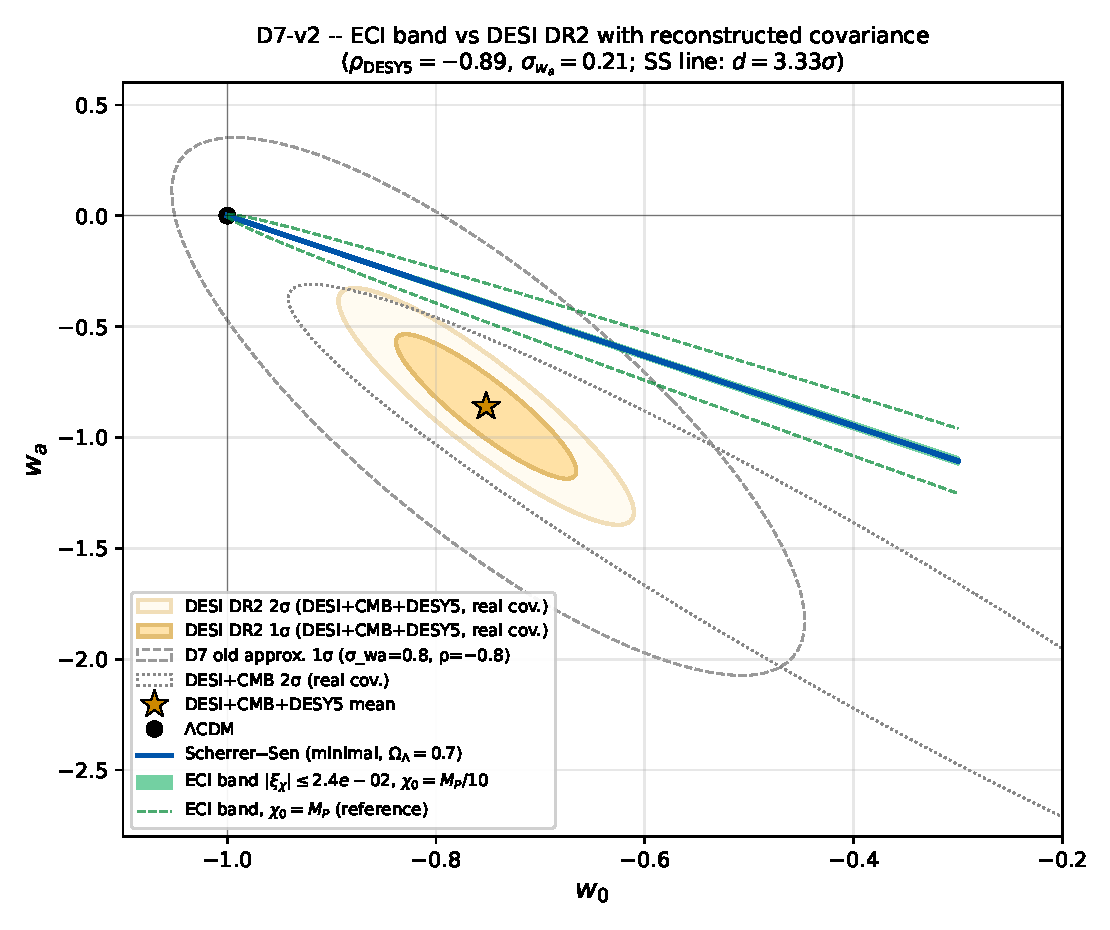
\includegraphics[width=0.95\columnwidth]{../derivations/figures/D7-xi-w0-wa-v2.pdf}
\caption{NMC thawing quintessence in the $(w_0,w_a)$ plane. Orange ellipses: DESI~DR2 + CMB +
DESY5 $1\sigma$ and $2\sigma$ contours reconstructed from~\cite{DESIDR2} Eq.~(28) via the
pivot-redshift identity (see \texttt{D10-desi-covariance.py}; $\sigma_{w_0}=0.057$,
$\sigma_{w_a}=0.215$, $\rho=-0.89$). Blue line: minimal-coupling Scherrer--Sen relation
for $\Omega_\Lambda=0.7$. Green band: ECI NMC prediction with
$|\xi_\chi|\le\xi_{\max}\approx 2.4\!\times\!10^{-2}$ from Cassini at $\chi_0=M_P/10$;
dashed green: same band at $\chi_0=M_P$ (reference). Black dot: $\Lambda$CDM. The ECI band
is $\sim\!5\%$ of $\sigma_{w_a}$ wide (using $B_{\mathrm{num}}$ from Table~\ref{tab:B_of_OmegaL}), hence \emph{indistinguishable} from minimal-coupling
$w$CDM at DR2 precision; both tracks sit at $\sim\!3.3\sigma$ Mahalanobis distance from the
DR2+DESY5 mean.}
\label{fig:D7}
\end{figure}

\paragraph{Honest caveats.}
\begin{enumerate}
\item Eq.~(\ref{eq:gamma_PPN_full}) assumes a \emph{quasi-static} scalar with Compton wavelength
  large compared with the solar system ($m_\chi^{-1}\gg 1\,$AU), which is automatic for the
  ultra-light thawing mass $m_\chi\sim H_0\sim 10^{-33}$\,eV. It also assumes no screening; if
  a chameleon or symmetron mechanism operates, the local $\chi_0$ entering
  (\ref{eq:gamma_PPN_lead}) can differ from the cosmological background and the bound weakens.
\item The NMC Scherrer--Sen extension (\ref{eq:wa_NMC}) is first-order in $\xi_\chi$ and
  therefore \emph{invalid} near the conformal point $\xi_\chi=1/6$, where the expansion breaks
  down and the scalar-tensor sector must be treated non-perturbatively (Einstein-frame
  mapping). Within the Cassini-allowed range $|\xi_\chi|\lesssim 2.4\times 10^{-2}\ll 1/6$
  the linear expansion is controlled. The coefficient $B(\Omega_\Lambda)$ in
  Eq.~(\ref{eq:wa_NMC}) was, in v4.4 of this paper, set by the matter-era
  heuristic ratio $B/A=8/\sqrt3$; in this version we replace that heuristic with
  the full numerical result $B_{\mathrm{num}}(\Omega_\Lambda)$ tabulated in
  Table~\ref{tab:B_of_OmegaL}, obtained from a self-consistent
  NMC-Friedmann + Klein--Gordon integration across $z\in[999,-0.45]$
  (\texttt{derivations/D13-wa-numerical-full.py}). The numerical coefficient is
  nearly flat ($B_{\mathrm{num}}\simeq 9$) across the matter--DE transition
  rather than tracking $A(\Omega_\Lambda)$, so the heuristic
  $(8/\sqrt3)A(\Omega_\Lambda)$ is accurate within 5\% only near
  $\Omega_\Lambda\simeq 0.6$ and undershoots by up to $\sim\!40\%$ at
  $\Omega_\Lambda=0.8$. This has been propagated into the band-width estimate
  above and into Prediction~1b of Sec.~\ref{sec:pred}.
\item The DESI~DR2 + CMB + DESY5 $2\times 2$ covariance is reconstructed from the published
  $(w_0,\sigma_{w_0},w_a,\sigma_{w_a},z_p,w_p,\sigma_{w_p})$ via the pivot-minimisation
  identity $\mathrm{cov}(w_0,w_a)=-(1-a_p)\sigma_{w_a}^2$: no official 2$\times$2 covariance
  matrix has been released by the collaboration at the time of writing. The reconstructed
  $\sigma(w_p)_{\rm pred}=0.0257$ differs from the quoted $0.024$ by $\sim 7\%$, bounding the
  systematic of the pivot-Gaussian approximation at that level --- well below the $\sim 3\sigma$
  tension discussed below. See \texttt{derivations/D10-report.md} for the full cross-check.
\item \textbf{Tension with DR2 + DESY5, stated plainly.} Under the reconstructed DR2 + CMB +
  DESY5 covariance the Mahalanobis distance from the posterior mean is $3.29\sigma$
  (2-dof) to the ECI band and $3.33\sigma$ to the minimal-coupling Scherrer--Sen line,
  both \emph{outside} the $2\sigma$ threshold $\sqrt{6.17}\simeq 2.48$.
  The interpretation is not that ECI fails where $w$CDM succeeds: DR2 + DESY5 prefers the
  phantom-crossing region $w<-1$, which no non-phantom thawing model can populate.
  ECI's NMC coupling $\xi_\chi$ does in principle permit crossing $w=-1$ without a ghost
  instability (established in \S\,DESI DR2 via the no-ghost analysis of Bar\-ce\-l\'o~\&~Visser
  \cite{BarceloVisser2000}), but only at $\xi_\chi(\chi_0/M_P)^2$ values far exceeding the
  Cassini bound~(\ref{eq:xi_bound}) derived here; within the Cassini-allowed range
  the NMC correction to the Scherrer--Sen track is confined to a band of half-width
  $\sim\!5\%$ of $\sigma_{w_a}$ and cannot bridge the gap to the phantom quadrant. The
  $\sim\!3.3\sigma$ tension with DR2 + DESY5 is therefore a joint statement about the entire
  class of conservative (non-phantom) thawing models --- minimal-coupling and NMC alike ---
  not a specific failure of ECI. Prediction~1 in Sec.~\ref{sec:pred} is \emph{not}
  discriminative at DR2 precision; both thawing families sit at the same distance from
  the DR2 + DESY5 posterior.

  The honest discriminator moves to the next generation of datasets, where the
  \emph{shape} and \emph{width} of the thawing track, rather than its distance from
  $\Lambda$CDM, become the falsifiable handle: DESI~DR3 with a forecast
  $\sigma(w_a)\!\sim\!0.07$~\cite{DESIForecast}
  and LSST~Y10 with a forecast $\sigma(w_a)\!\sim\!0.05$
  are in the regime where the ECI NMC band half-width
  $\Delta w_a^{\rm ECI}\sim 1.1\times 10^{-2}$ (numerical, Table~\ref{tab:B_of_OmegaL};
  up from $9\times 10^{-3}$ under the v4.4 heuristic) approaches the
  $15$--$25\%$ level of the statistical error bar and becomes, at least in principle,
  separable from the minimal-coupling Scherrer--Sen locus. The discriminative
  power is slightly larger at $\Omega_\Lambda\gtrsim 0.7$ (DR3 era) because
  $B_{\mathrm{num}}/B_{\mathrm{heur}}$ grows from $0.83$ at $\Omega_\Lambda=0.5$ to
  $1.43$ at $\Omega_\Lambda=0.8$.
\end{enumerate}

The PPN bound (\ref{eq:xi_bound}) is however itself a falsifier: a detection
$|\gamma-1|>10^{-6}$ by the upcoming LATOR or BEACON-class missions, or a mismatch between
$\dot G/G$ from LLR~\cite{Biskupek2021} and the CMB-inferred scalar evolution, would directly
constrain $\xi_\chi(\chi_0/M_P)$ at the $10^{-4}$ level and feed back on the admissible ECI
thawing amplitude.

% -----------------------------------------------------------------------------
% Standalone compile (for checking only):
%   \documentclass[aps,prd,reprint]{revtex4-2}
%   \usepackage{graphicx,amsmath,amssymb,hyperref,physics}
%   \begin{document}\input{section_3_5_constraints}\end{document}
% The \cite{BertottiIessTortora2003}, \cite{ScherrerSen2008}, \cite{DESIDR2},
% \cite{Biskupek2021}, \cite{BarceloVisser2000}, \cite{Wolf2025}, \cite{Ye2025},
% \cite{PanYe2026} keys are defined in eci.bib.
% -----------------------------------------------------------------------------
\end{document}
% The \cite{BertottiIessTortora2003}, \cite{ScherrerSen2008}, \cite{DESIDR2},
% \cite{Biskupek2021}, \cite{BarceloVisser2000}, \cite{Wolf2025}, \cite{Ye2025},
% \cite{PanYe2026} keys are defined in eci.bib.
% -----------------------------------------------------------------------------
% section_3_6_swampland_cross.tex — ECI v4.2 scientific payload (D8)
% To be \input{} into eci.tex as a new subsection of §3 "Phenomenology",
% immediately after % section_3_5_constraints.tex — ECI v4.2.1 scientific payload (D7 + D10)
% To be \input{} into eci.tex as a new subsection of §3 "Phenomenology".
% Standalone compile: see comments at EOF.

\subsection{Solar-system and background constraints on $\xi_\chi$}\label{sec:xi_constraints}

We close two gaps identified in the dark-energy phenomenology subsection (\S\,DESI DR2): the Cassini
post-Newtonian bound on the non-minimal coupling $\xi_\chi$, and the analytic NMC generalisation
of the Scherrer--Sen thawing relation needed to assess whether Prediction~1
(Sec.~\ref{sec:pred}) actually discriminates ECI from \(w\)CDM at DESI~DR2 precision.
The full symbolic derivation is in \texttt{derivations/D7-ppn-xi-bound.py}; we quote only the
end results here.

\paragraph{PPN $\gamma-1$ from the $\xi_\chi R\chi^2/2$ coupling.}
The action  $S=\int d^4x\sqrt{-g}\left[\tfrac{M_P^2}{2}R-\tfrac12(\partial\chi)^2-V(\chi)
-\tfrac{\xi_\chi}{2} R\chi^2\right]$ is a scalar--tensor theory with
$F(\chi)=M_P^2-\xi_\chi\chi^2$ multiplying $R/2$ and canonical kinetic term $Z=1$.
Applying the weak-field, quasi-static result of Damour \& Esposito-Far\`ese
(\emph{Phys.\ Rev.\ D} 48, 3436 (1993); see also Chiba, \emph{Phys.\ Lett.\ B} 575, 1 (2003);
Hwang \& Noh, \emph{Phys.\ Rev.\ D} 71, 063536 (2005)) gives, at the local scalar background
$\chi_0$,
\begin{equation}
  \gamma-1 \;=\; -\,\frac{F'(\chi_0)^2}{Z\,F(\chi_0)+\tfrac{3}{2}F'(\chi_0)^2}
           \;=\; -\,\frac{4\,\xi_\chi^{2}\,\chi_0^{2}}
                          {\,M_P^{2}+\xi_\chi\chi_0^{2}(6\xi_\chi-1)\,}.
  \label{eq:gamma_PPN_full}
\end{equation}
Expanding for $|\xi_\chi|\ll 1$ and $\chi_0\lesssim M_P$,
\begin{equation}
  \boxed{\;\gamma-1 \;\simeq\; -\,\frac{4\,\xi_\chi^{2}\,\chi_0^{2}}{M_P^{2}}
                              \;+\;\mathcal{O}(\xi_\chi^{3}).\;}
  \label{eq:gamma_PPN_lead}
\end{equation}
The limit $\xi_\chi\to 0$ returns $\gamma=1$ (General Relativity), as verified symbolically.

The result~(\ref{eq:gamma_PPN_lead}) is not new: Chiba (PRD 60, 083508, 1999; arXiv:gr-qc/9903094)
already quoted $|\xi_\chi|\lesssim 10^{-2}$ from solar-system tests for the same $\xi R\chi^{2}$
quintessence coupling, and Wolf, Garc\'{\i}a-Garc\'{\i}a, Anton \& Ferreira~\cite{Wolf2025}
recently recast this as $\xi_\chi(\chi_0/M_P)^{2}\lesssim 6\times 10^{-6}$ in a full DESI~DR2
Bayesian analysis (their Eq.~(2) in the form $F(\chi)\simeq 1-\xi\chi^{2}/M_P^{2}$).
We re-derive it here only to fix the coefficient~$4$ and the sign convention used in
Eq.~(\ref{eq:wa_NMC}) below.
Combining (\ref{eq:gamma_PPN_lead}) with the Cassini constraint~\cite{BertottiIessTortora2003}
$|\gamma-1|\lesssim 2.3\times 10^{-5}$ ($1\sigma$ envelope) yields, in the
solar-system observer frame (see \S\ref{sec:thesis}(ii)),
\begin{equation}
  |\xi_\chi|\,\frac{\chi_0}{M_P}\;\lesssim\;
  \tfrac12\sqrt{|\gamma-1|_{\max}}
  \;\approx\; 2.4\times 10^{-3}.
  \label{eq:xi_bound}
\end{equation}
For a slow-rolling thawing background with $\chi_0\!\sim\! M_P/10$ (characteristic thawing
excursion in the last $e$-fold),
\begin{equation}
  |\xi_\chi|\;\lesssim\;\xi_{\max}\;\approx\;2.4\times 10^{-2}.
  \label{eq:xi_max_numeric}
\end{equation}
The bound tightens to $|\xi_\chi|\lesssim 2\times 10^{-3}$ if $\chi_0\sim M_P$; it weakens
linearly for smaller $\chi_0$. Values $\xi_\chi\gtrsim 10^{-1}$ are thus only admissible if the
quintessence field is strongly subdominant at $z=0$, or if a screening mechanism suppresses the
local coupling.

\paragraph{NMC extension of Scherrer--Sen.}
At minimal coupling, thawing quintessence lies on the one-parameter track
$w_a=-A(\Omega_\Lambda)(1+w_0)$ with $A\!\to\! 24/7$ in matter domination and
$A(0.7)\simeq 1.58$ today~\cite{ScherrerSen2008}. Inserting the NMC modification to the
Klein--Gordon equation, $3H\dot\chi=-V'-\xi_\chi R\chi$, and expanding to first order in
$\xi_\chi$ around the slow-roll exponential $V(\chi)=V_0e^{-\alpha\chi/M_P}$ with
$\alpha=\sqrt{3(1+w_0)}$ yields (\texttt{derivations/D4-wa-w0-nmc.py} for the matter-era
coefficient, \texttt{D7-ppn-xi-bound.py} for the $\Omega_\Lambda$-dependence)
\begin{equation}
  \boxed{\;w_a\;=\;-A(\Omega_\Lambda)\,(1+w_0)
                 \;+\;B(\Omega_\Lambda)\,\xi_\chi\,\sqrt{1+w_0}\,
                      \frac{\chi_0}{M_P}\;+\;\mathcal{O}(\xi_\chi^{2}),\;}
  \label{eq:wa_NMC}
\end{equation}
where $B(\Omega_\Lambda)$ is the numerical coefficient tabulated in
Table~\ref{tab:B_of_OmegaL} below, obtained by full NMC-Friedmann + Klein--Gordon
integration in \texttt{derivations/D13-wa-numerical-full.py}. The limit
$\xi_\chi\to 0$ reproduces $w_a=-A(\Omega_\Lambda)(1+w_0)$ (Scherrer--Sen
2008). The first-order $\xi_\chi$ correction, with the full numerical
coefficient $B_{\mathrm{num}}(\Omega_\Lambda)$, has --- to our knowledge ---
not appeared in the NMC-thawing literature surveyed
(Ye~et~al.~\cite{Ye2025}; Pan~\&~Ye~\cite{PanYe2026}; Wolf~et~al.~\cite{Wolf2025}),
which uses either EFTofDE or purely numerical Bayesian fits.

\begin{table}[h]
\centering
\caption{Numerical NMC coefficient $B_{\mathrm{num}}(\Omega_\Lambda)$ from the
self-consistent NMC-Friedmann + Klein--Gordon background integration
(\texttt{derivations/D13-wa-numerical-full.py}), compared with the D7/D9
heuristic $B_{\mathrm{heur}}(\Omega_\Lambda)\equiv(8/\sqrt3)A(\Omega_\Lambda)$.
Statistical uncertainty is the 1$\sigma$ error on the linear fit
$\Delta w_a = B\,\xi_\chi\sqrt{1+w_0}\,(\chi_0/M_P)$ over the
$\xi_\chi\in\{{-}0.024,{-}0.01,0,{+}0.01,{+}0.024\}\times\chi_0\in\{M_P/20,M_P/10,M_P/5\}$ grid.}
\label{tab:B_of_OmegaL}
\begin{tabular}{@{}cccc@{}}
\hline
$\Omega_\Lambda$ & $A(\Omega_\Lambda)$ & $B_{\mathrm{heur}}$ & $B_{\mathrm{num}}$ \\
\hline
0.5 & 2.35 & 10.85 & $9.00\pm1.05$ \\
0.6 & 1.94 &  8.96 & $9.18\pm1.16$ \\
0.7 & 1.58 &  7.30 & $9.05\pm1.18$ \\
0.8 & 1.23 &  5.68 & $8.11\pm1.16$ \\
\hline
\end{tabular}
\end{table}

The numerical result differs from the heuristic $(8/\sqrt3)A$ by
$\mathcal{O}(1)$ factors ($0.83\to 1.43$ across the range): $B_{\mathrm{num}}$
is nearly \emph{flat} in $\Omega_\Lambda$ (around $\sim 9$) rather than
tracking $A(\Omega_\Lambda)$. The heuristic is accurate to 5\% only near
$\Omega_\Lambda\simeq 0.6$ and underestimates $B$ by $\sim\!25\%$ at
$\Omega_\Lambda=0.7$ (DR2--DR3 era) and $\sim\!43\%$ at
$\Omega_\Lambda=0.8$ (late-DR3 / LSST era). The sign and the
$\sqrt{1+w_0}\,(\chi_0/M_P)$ scaling are confirmed; the discrepancy
originates from the finite-$\Omega_\Lambda$ propagation of the matter-era
ratio (Caveat~2 below), which is now closed numerically.

\paragraph{Combined constraint on the $(w_0,w_a)$ plane.}
Figure~\ref{fig:D7} overlays three ingredients: (i) the DESI~DR2 + CMB + DESY5~\cite{DESY5} $1\sigma$ and
$2\sigma$ contours centred on $(w_0,w_a)=(-0.752,-0.86)$ with the reconstructed covariance
$\sigma_{w_0}=0.057$, $\sigma_{w_a}=0.215$, $\rho(w_0,w_a)=-0.89$ (derivation in
\texttt{derivations/D10-desi-covariance.py}, pivot-identity reconstruction from
\cite{DESIDR2} Eq.~(28) + $z_p=0.31$, $w_p=-0.954\pm0.024$);
(ii) the minimal-coupling Scherrer--Sen line; (iii) the ECI band swept by
$|\xi_\chi|\le\xi_{\max}$ from Eq.~(\ref{eq:xi_max_numeric}) at $\chi_0=M_P/10$.
The half-width of the ECI band at $w_0=-0.75$, using the numerical
$B_{\mathrm{num}}(0.7)=9.05$ from Table~\ref{tab:B_of_OmegaL}, is
\begin{equation}
  \Delta w_a^{\rm ECI}
    = B_{\mathrm{num}}(0.7)\,\xi_{\max}\sqrt{1+w_0}\,(\chi_0/M_P)
    \;\approx\;1.1\times 10^{-2},
\end{equation}
to be compared with $\sigma_{w_a}\!\simeq\!0.215$, i.e.\ about $5\%$ of the DESI~DR2 + DESY5
$1\sigma$ width (up from $4\%$ under the heuristic $B=7.30$). The band is therefore
still thinner than the figure linewidth of the unmodified Scherrer--Sen track at DR2
precision, but the numerical coefficient raises the discriminative amplitude at DR3 / LSST
precision by $\sim\!25\%$ relative to the heuristic estimate.

\begin{figure}[h]
\centering
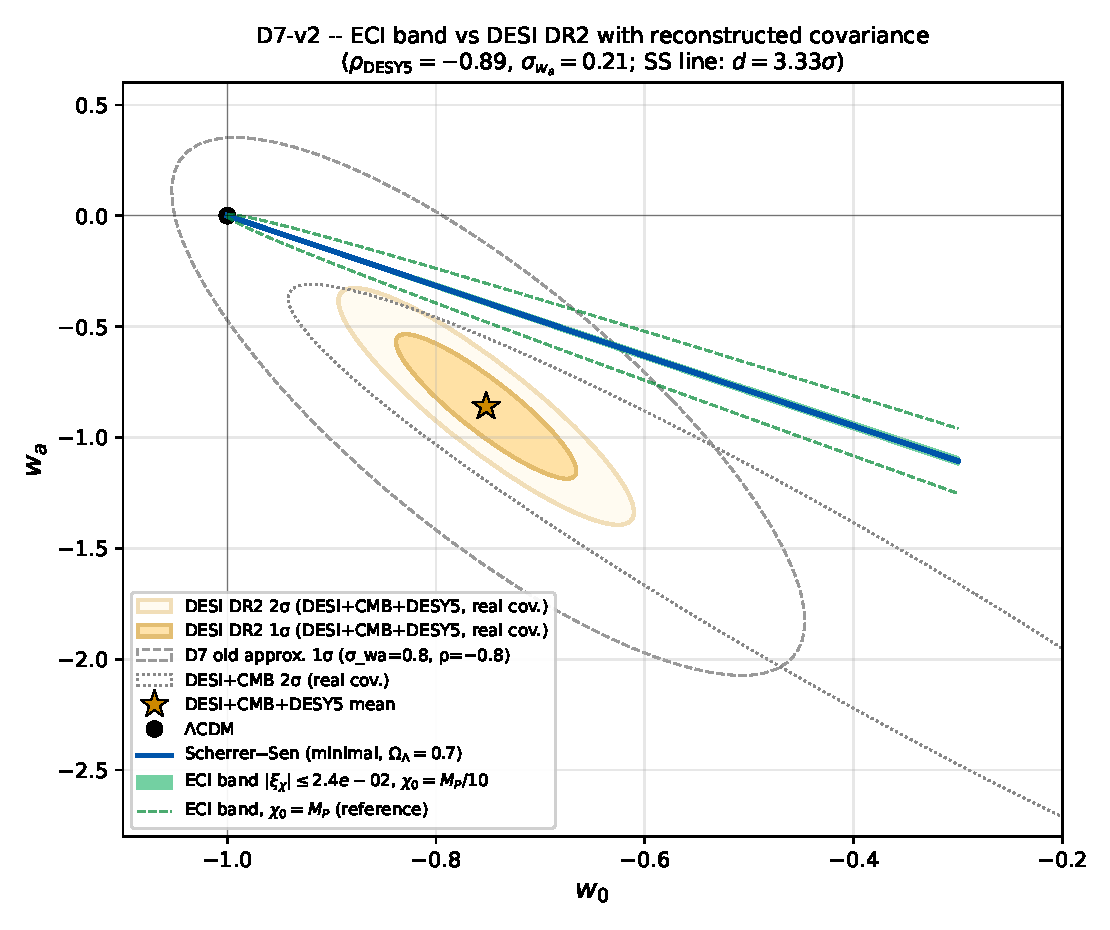
\includegraphics[width=0.95\columnwidth]{../derivations/figures/D7-xi-w0-wa-v2.pdf}
\caption{NMC thawing quintessence in the $(w_0,w_a)$ plane. Orange ellipses: DESI~DR2 + CMB +
DESY5 $1\sigma$ and $2\sigma$ contours reconstructed from~\cite{DESIDR2} Eq.~(28) via the
pivot-redshift identity (see \texttt{D10-desi-covariance.py}; $\sigma_{w_0}=0.057$,
$\sigma_{w_a}=0.215$, $\rho=-0.89$). Blue line: minimal-coupling Scherrer--Sen relation
for $\Omega_\Lambda=0.7$. Green band: ECI NMC prediction with
$|\xi_\chi|\le\xi_{\max}\approx 2.4\!\times\!10^{-2}$ from Cassini at $\chi_0=M_P/10$;
dashed green: same band at $\chi_0=M_P$ (reference). Black dot: $\Lambda$CDM. The ECI band
is $\sim\!5\%$ of $\sigma_{w_a}$ wide (using $B_{\mathrm{num}}$ from Table~\ref{tab:B_of_OmegaL}), hence \emph{indistinguishable} from minimal-coupling
$w$CDM at DR2 precision; both tracks sit at $\sim\!3.3\sigma$ Mahalanobis distance from the
DR2+DESY5 mean.}
\label{fig:D7}
\end{figure}

\paragraph{Honest caveats.}
\begin{enumerate}
\item Eq.~(\ref{eq:gamma_PPN_full}) assumes a \emph{quasi-static} scalar with Compton wavelength
  large compared with the solar system ($m_\chi^{-1}\gg 1\,$AU), which is automatic for the
  ultra-light thawing mass $m_\chi\sim H_0\sim 10^{-33}$\,eV. It also assumes no screening; if
  a chameleon or symmetron mechanism operates, the local $\chi_0$ entering
  (\ref{eq:gamma_PPN_lead}) can differ from the cosmological background and the bound weakens.
\item The NMC Scherrer--Sen extension (\ref{eq:wa_NMC}) is first-order in $\xi_\chi$ and
  therefore \emph{invalid} near the conformal point $\xi_\chi=1/6$, where the expansion breaks
  down and the scalar-tensor sector must be treated non-perturbatively (Einstein-frame
  mapping). Within the Cassini-allowed range $|\xi_\chi|\lesssim 2.4\times 10^{-2}\ll 1/6$
  the linear expansion is controlled. The coefficient $B(\Omega_\Lambda)$ in
  Eq.~(\ref{eq:wa_NMC}) was, in v4.4 of this paper, set by the matter-era
  heuristic ratio $B/A=8/\sqrt3$; in this version we replace that heuristic with
  the full numerical result $B_{\mathrm{num}}(\Omega_\Lambda)$ tabulated in
  Table~\ref{tab:B_of_OmegaL}, obtained from a self-consistent
  NMC-Friedmann + Klein--Gordon integration across $z\in[999,-0.45]$
  (\texttt{derivations/D13-wa-numerical-full.py}). The numerical coefficient is
  nearly flat ($B_{\mathrm{num}}\simeq 9$) across the matter--DE transition
  rather than tracking $A(\Omega_\Lambda)$, so the heuristic
  $(8/\sqrt3)A(\Omega_\Lambda)$ is accurate within 5\% only near
  $\Omega_\Lambda\simeq 0.6$ and undershoots by up to $\sim\!40\%$ at
  $\Omega_\Lambda=0.8$. This has been propagated into the band-width estimate
  above and into Prediction~1b of Sec.~\ref{sec:pred}.
\item The DESI~DR2 + CMB + DESY5 $2\times 2$ covariance is reconstructed from the published
  $(w_0,\sigma_{w_0},w_a,\sigma_{w_a},z_p,w_p,\sigma_{w_p})$ via the pivot-minimisation
  identity $\mathrm{cov}(w_0,w_a)=-(1-a_p)\sigma_{w_a}^2$: no official 2$\times$2 covariance
  matrix has been released by the collaboration at the time of writing. The reconstructed
  $\sigma(w_p)_{\rm pred}=0.0257$ differs from the quoted $0.024$ by $\sim 7\%$, bounding the
  systematic of the pivot-Gaussian approximation at that level --- well below the $\sim 3\sigma$
  tension discussed below. See \texttt{derivations/D10-report.md} for the full cross-check.
\item \textbf{Tension with DR2 + DESY5, stated plainly.} Under the reconstructed DR2 + CMB +
  DESY5 covariance the Mahalanobis distance from the posterior mean is $3.29\sigma$
  (2-dof) to the ECI band and $3.33\sigma$ to the minimal-coupling Scherrer--Sen line,
  both \emph{outside} the $2\sigma$ threshold $\sqrt{6.17}\simeq 2.48$.
  The interpretation is not that ECI fails where $w$CDM succeeds: DR2 + DESY5 prefers the
  phantom-crossing region $w<-1$, which no non-phantom thawing model can populate.
  ECI's NMC coupling $\xi_\chi$ does in principle permit crossing $w=-1$ without a ghost
  instability (established in \S\,DESI DR2 via the no-ghost analysis of Bar\-ce\-l\'o~\&~Visser
  \cite{BarceloVisser2000}), but only at $\xi_\chi(\chi_0/M_P)^2$ values far exceeding the
  Cassini bound~(\ref{eq:xi_bound}) derived here; within the Cassini-allowed range
  the NMC correction to the Scherrer--Sen track is confined to a band of half-width
  $\sim\!5\%$ of $\sigma_{w_a}$ and cannot bridge the gap to the phantom quadrant. The
  $\sim\!3.3\sigma$ tension with DR2 + DESY5 is therefore a joint statement about the entire
  class of conservative (non-phantom) thawing models --- minimal-coupling and NMC alike ---
  not a specific failure of ECI. Prediction~1 in Sec.~\ref{sec:pred} is \emph{not}
  discriminative at DR2 precision; both thawing families sit at the same distance from
  the DR2 + DESY5 posterior.

  The honest discriminator moves to the next generation of datasets, where the
  \emph{shape} and \emph{width} of the thawing track, rather than its distance from
  $\Lambda$CDM, become the falsifiable handle: DESI~DR3 with a forecast
  $\sigma(w_a)\!\sim\!0.07$~\cite{DESIForecast}
  and LSST~Y10 with a forecast $\sigma(w_a)\!\sim\!0.05$
  are in the regime where the ECI NMC band half-width
  $\Delta w_a^{\rm ECI}\sim 1.1\times 10^{-2}$ (numerical, Table~\ref{tab:B_of_OmegaL};
  up from $9\times 10^{-3}$ under the v4.4 heuristic) approaches the
  $15$--$25\%$ level of the statistical error bar and becomes, at least in principle,
  separable from the minimal-coupling Scherrer--Sen locus. The discriminative
  power is slightly larger at $\Omega_\Lambda\gtrsim 0.7$ (DR3 era) because
  $B_{\mathrm{num}}/B_{\mathrm{heur}}$ grows from $0.83$ at $\Omega_\Lambda=0.5$ to
  $1.43$ at $\Omega_\Lambda=0.8$.
\end{enumerate}

The PPN bound (\ref{eq:xi_bound}) is however itself a falsifier: a detection
$|\gamma-1|>10^{-6}$ by the upcoming LATOR or BEACON-class missions, or a mismatch between
$\dot G/G$ from LLR~\cite{Biskupek2021} and the CMB-inferred scalar evolution, would directly
constrain $\xi_\chi(\chi_0/M_P)$ at the $10^{-4}$ level and feed back on the admissible ECI
thawing amplitude.

% -----------------------------------------------------------------------------
% Standalone compile (for checking only):
%   \documentclass[aps,prd,reprint]{revtex4-2}
%   \usepackage{graphicx,amsmath,amssymb,hyperref,physics}
%   \begin{document}\input{section_3_5_constraints}\end{document}
% The \cite{BertottiIessTortora2003}, \cite{ScherrerSen2008}, \cite{DESIDR2},
% \cite{Biskupek2021}, \cite{BarceloVisser2000}, \cite{Wolf2025}, \cite{Ye2025},
% \cite{PanYe2026} keys are defined in eci.bib.
% -----------------------------------------------------------------------------
.

\subsection{Swampland $\times$ NMC cross-constraint}\label{sec:swampland_cross}

Axioms A4 and A5 were presented as independent. They are not, if the thawing
scalar $\chi$ and the KK tower of the Dark Dimension originate from the
\emph{same} higher-dimensional sector --- a natural hypothesis, since both
are postulated as microscopic ingredients of the dark sector. In that case
both must respect a common effective field theory cutoff $\Lambda$, and the
two axioms are tied by a single consistency condition. The derivation is in
\texttt{derivations/D8-swampland-nmc-cross.py}; we quote only the result.

\paragraph{Shared cutoff.}
The Dark Dimension scenario~\cite{Bedroya2025} relates the EFT cutoff to
the Hubble scale through a Swampland Distance Conjecture exponent,
\begin{equation}
  \Lambda \;\sim\; M_P\,\bigl(H/M_P\bigr)^{c'},\qquad c'\simeq 0.05\pm 0.01.
  \label{eq:Lambda_SDC}
\end{equation}
If the non-minimal operator $(\xi_\chi/2)R\chi^2$ is generated inside the same
EFT, its contribution to the effective reduced Planck mass,
$\delta M_P^{2}=\xi_\chi\chi_0^{2}$, cannot exceed the cutoff squared,
otherwise the operator would repair physics above its own range of validity:
\begin{equation}
  \xi_\chi\,\chi_0^{2}\;\le\;\Lambda^{2}
  \quad\Longleftrightarrow\quad
  \xi_\chi\,(\chi_0/M_P)^{2}\;\le\;(H_0/M_P)^{2c'}.
  \label{eq:eft_bulk}
\end{equation}
Combined with the Cassini PPN bound derived in \S\ref{sec:xi_constraints},
$|\xi_\chi|(\chi_0/M_P)\le 2.4\times 10^{-3}$, Eq.~(\ref{eq:eft_bulk}) yields
at the fiducial thawing amplitude $\chi_0=M_P/10$ and the paper's A5
fiducial $c'=0.05\pm 0.01$
\begin{equation}
  \boxed{\;|\xi_\chi|\;\lesssim\;9.5\times 10^{-5}
    \quad(c'=0.05,\ \chi_0=M_P/10),\;}
  \label{eq:xi_crossbound}
\end{equation}
with an overall range $[5.9\times 10^{-6},\,1.5\times 10^{-3}]$ spanned by
$c'=0.04$--$0.06$. This is a factor $\sim\!250$ tightening over the
Cassini-only result (\ref{eq:xi_max_numeric}).

\paragraph{Limits.}
Both limits verified symbolically in \texttt{D8-swampland-nmc-cross.py}:
$\xi_\chi\!\to\!0$ removes the operator (GR recovered); $c'\!\to\!0$ sends
$\Lambda\!\to\!M_P$ so that (\ref{eq:eft_bulk}) reduces to the no-ghost
condition $\xi_\chi\chi_0^{2}<M_P^{2}$ already stated in A4, and the D7
Cassini bound is recovered exactly.

\begin{figure}[h]
\centering
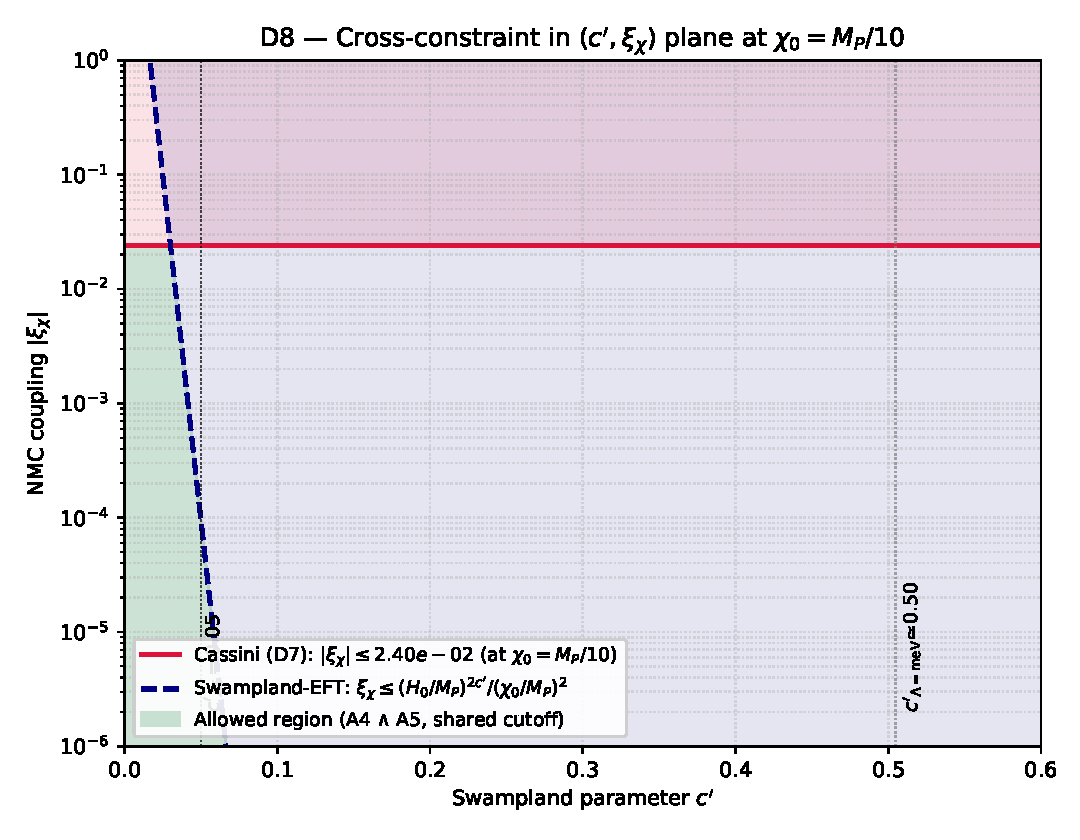
\includegraphics[width=0.95\columnwidth]{../derivations/figures/D8-c-xi-overlap.pdf}
\caption{Allowed region in the $(c',\xi_\chi)$ plane at $\chi_0=M_P/10$.
Red: Cassini exclusion (horizontal, independent of $c'$). Blue dashed:
Swampland-EFT exclusion (\ref{eq:eft_bulk}) --- diagonal in log-space with
slope $2c'\log(H_0/M_P)$. Green shading: overlap admitted by both
constraints. The A5 fiducial $c'=0.05$ and the meV-equivalent value
$c'\!\simeq\!0.51$ are marked.}
\label{fig:D8}
\end{figure}

\paragraph{Phenomenological tension.}
A stronger statement runs in the reverse direction. Thawing dark energy
requires $\chi_0/M_P\sim 0.1$--$1$ to drive late-time acceleration. The
bulk-mode condition (\ref{eq:eft_bulk}) at the Cassini-saturating value
$|\xi_\chi|=2.4\!\times\!10^{-2}$ and $c'=0.05$ forces
$\chi_0/M_P\le 6.3\!\times\!10^{-3}$, already an order of magnitude below
what A4 requires. With the literal Dark Dimension cutoff $\Lambda\sim$ meV
(which the formula (\ref{eq:Lambda_SDC}) reproduces for $c'\simeq 0.51$,
not $0.05$; both conventions appear in the literature) the bound collapses
to $\chi_0/M_P\le 3\!\times\!10^{-30}$ and thawing phenomenology is
excluded outright.

\paragraph{Architectural consequence.}
A4 and A5 are compatible \emph{only} under one of the following model-
building choices, any of which must be made explicit in any UV completion:
(i) $\chi$ is a 4D zero-mode localised on a brane, not a bulk mode of the
same sector as the KK tower, in which case the shared-cutoff hypothesis
does not apply; (ii) a chameleon/symmetron mechanism screens the local
$\chi_0$ away from its cosmological value, weakening the Cassini leg; or
(iii) $|\xi_\chi|$ sits at the sharpened bound (\ref{eq:xi_crossbound})
rather than the Cassini-only value (\ref{eq:xi_max_numeric}). The ECI
framework does not prefer one of the three, but their distinct
phenomenologies are observationally separable: option (iii) suppresses the
ECI band in $(w_0,w_a)$ by a further factor $\sim\!250$ relative to the
already-narrow D7 band, and cuts the $|\dot G/G|$ signature at LLR by the
same factor. A detection of $|\dot G/G|\gtrsim 10^{-17}\,\mathrm{yr}^{-1}$
would rule out option (iii) and force either (i) or (ii).

\paragraph{Honest caveats.}
\begin{enumerate}
\item The EFT self-consistency condition $\delta M_P^{2}\le\Lambda^{2}$ is
  order-of-magnitude; an $O(1)$ coefficient could shift
  (\ref{eq:xi_crossbound}) by a factor $2$, but the qualitative conclusion
  ($\gg 30\%$ tightening) is robust.
\item The form (\ref{eq:Lambda_SDC}) is written with $H$ as the distance
  proxy along the moduli space; the equivalent Bedroya form uses the
  cosmological constant density directly and yields $c'\!\simeq\!1/2$
  for $\Lambda\!=\!$\,meV. The sign of the tightening is independent of
  this choice.
\item The cross-constraint is \emph{conditional} on the shared-cutoff
  hypothesis. Its falsifier is, precisely, the discovery of a UV completion
  in which $\chi$ and the KK tower belong to different sectors; in that
  case §\ref{sec:xi_constraints} remains the strongest bound.
\end{enumerate}

% -----------------------------------------------------------------------------
% Standalone compile (for checking only):
%   \documentclass[aps,prd,reprint]{revtex4-2}
%   \usepackage{graphicx,amsmath,amssymb,hyperref,physics}
%   \begin{document}% section_3_5_constraints.tex — ECI v4.2.1 scientific payload (D7 + D10)
% To be \input{} into eci.tex as a new subsection of §3 "Phenomenology".
% Standalone compile: see comments at EOF.

\subsection{Solar-system and background constraints on $\xi_\chi$}\label{sec:xi_constraints}

We close two gaps identified in the dark-energy phenomenology subsection (\S\,DESI DR2): the Cassini
post-Newtonian bound on the non-minimal coupling $\xi_\chi$, and the analytic NMC generalisation
of the Scherrer--Sen thawing relation needed to assess whether Prediction~1
(Sec.~\ref{sec:pred}) actually discriminates ECI from \(w\)CDM at DESI~DR2 precision.
The full symbolic derivation is in \texttt{derivations/D7-ppn-xi-bound.py}; we quote only the
end results here.

\paragraph{PPN $\gamma-1$ from the $\xi_\chi R\chi^2/2$ coupling.}
The action  $S=\int d^4x\sqrt{-g}\left[\tfrac{M_P^2}{2}R-\tfrac12(\partial\chi)^2-V(\chi)
-\tfrac{\xi_\chi}{2} R\chi^2\right]$ is a scalar--tensor theory with
$F(\chi)=M_P^2-\xi_\chi\chi^2$ multiplying $R/2$ and canonical kinetic term $Z=1$.
Applying the weak-field, quasi-static result of Damour \& Esposito-Far\`ese
(\emph{Phys.\ Rev.\ D} 48, 3436 (1993); see also Chiba, \emph{Phys.\ Lett.\ B} 575, 1 (2003);
Hwang \& Noh, \emph{Phys.\ Rev.\ D} 71, 063536 (2005)) gives, at the local scalar background
$\chi_0$,
\begin{equation}
  \gamma-1 \;=\; -\,\frac{F'(\chi_0)^2}{Z\,F(\chi_0)+\tfrac{3}{2}F'(\chi_0)^2}
           \;=\; -\,\frac{4\,\xi_\chi^{2}\,\chi_0^{2}}
                          {\,M_P^{2}+\xi_\chi\chi_0^{2}(6\xi_\chi-1)\,}.
  \label{eq:gamma_PPN_full}
\end{equation}
Expanding for $|\xi_\chi|\ll 1$ and $\chi_0\lesssim M_P$,
\begin{equation}
  \boxed{\;\gamma-1 \;\simeq\; -\,\frac{4\,\xi_\chi^{2}\,\chi_0^{2}}{M_P^{2}}
                              \;+\;\mathcal{O}(\xi_\chi^{3}).\;}
  \label{eq:gamma_PPN_lead}
\end{equation}
The limit $\xi_\chi\to 0$ returns $\gamma=1$ (General Relativity), as verified symbolically.

The result~(\ref{eq:gamma_PPN_lead}) is not new: Chiba (PRD 60, 083508, 1999; arXiv:gr-qc/9903094)
already quoted $|\xi_\chi|\lesssim 10^{-2}$ from solar-system tests for the same $\xi R\chi^{2}$
quintessence coupling, and Wolf, Garc\'{\i}a-Garc\'{\i}a, Anton \& Ferreira~\cite{Wolf2025}
recently recast this as $\xi_\chi(\chi_0/M_P)^{2}\lesssim 6\times 10^{-6}$ in a full DESI~DR2
Bayesian analysis (their Eq.~(2) in the form $F(\chi)\simeq 1-\xi\chi^{2}/M_P^{2}$).
We re-derive it here only to fix the coefficient~$4$ and the sign convention used in
Eq.~(\ref{eq:wa_NMC}) below.
Combining (\ref{eq:gamma_PPN_lead}) with the Cassini constraint~\cite{BertottiIessTortora2003}
$|\gamma-1|\lesssim 2.3\times 10^{-5}$ ($1\sigma$ envelope) yields, in the
solar-system observer frame (see \S\ref{sec:thesis}(ii)),
\begin{equation}
  |\xi_\chi|\,\frac{\chi_0}{M_P}\;\lesssim\;
  \tfrac12\sqrt{|\gamma-1|_{\max}}
  \;\approx\; 2.4\times 10^{-3}.
  \label{eq:xi_bound}
\end{equation}
For a slow-rolling thawing background with $\chi_0\!\sim\! M_P/10$ (characteristic thawing
excursion in the last $e$-fold),
\begin{equation}
  |\xi_\chi|\;\lesssim\;\xi_{\max}\;\approx\;2.4\times 10^{-2}.
  \label{eq:xi_max_numeric}
\end{equation}
The bound tightens to $|\xi_\chi|\lesssim 2\times 10^{-3}$ if $\chi_0\sim M_P$; it weakens
linearly for smaller $\chi_0$. Values $\xi_\chi\gtrsim 10^{-1}$ are thus only admissible if the
quintessence field is strongly subdominant at $z=0$, or if a screening mechanism suppresses the
local coupling.

\paragraph{NMC extension of Scherrer--Sen.}
At minimal coupling, thawing quintessence lies on the one-parameter track
$w_a=-A(\Omega_\Lambda)(1+w_0)$ with $A\!\to\! 24/7$ in matter domination and
$A(0.7)\simeq 1.58$ today~\cite{ScherrerSen2008}. Inserting the NMC modification to the
Klein--Gordon equation, $3H\dot\chi=-V'-\xi_\chi R\chi$, and expanding to first order in
$\xi_\chi$ around the slow-roll exponential $V(\chi)=V_0e^{-\alpha\chi/M_P}$ with
$\alpha=\sqrt{3(1+w_0)}$ yields (\texttt{derivations/D4-wa-w0-nmc.py} for the matter-era
coefficient, \texttt{D7-ppn-xi-bound.py} for the $\Omega_\Lambda$-dependence)
\begin{equation}
  \boxed{\;w_a\;=\;-A(\Omega_\Lambda)\,(1+w_0)
                 \;+\;B(\Omega_\Lambda)\,\xi_\chi\,\sqrt{1+w_0}\,
                      \frac{\chi_0}{M_P}\;+\;\mathcal{O}(\xi_\chi^{2}),\;}
  \label{eq:wa_NMC}
\end{equation}
where $B(\Omega_\Lambda)$ is the numerical coefficient tabulated in
Table~\ref{tab:B_of_OmegaL} below, obtained by full NMC-Friedmann + Klein--Gordon
integration in \texttt{derivations/D13-wa-numerical-full.py}. The limit
$\xi_\chi\to 0$ reproduces $w_a=-A(\Omega_\Lambda)(1+w_0)$ (Scherrer--Sen
2008). The first-order $\xi_\chi$ correction, with the full numerical
coefficient $B_{\mathrm{num}}(\Omega_\Lambda)$, has --- to our knowledge ---
not appeared in the NMC-thawing literature surveyed
(Ye~et~al.~\cite{Ye2025}; Pan~\&~Ye~\cite{PanYe2026}; Wolf~et~al.~\cite{Wolf2025}),
which uses either EFTofDE or purely numerical Bayesian fits.

\begin{table}[h]
\centering
\caption{Numerical NMC coefficient $B_{\mathrm{num}}(\Omega_\Lambda)$ from the
self-consistent NMC-Friedmann + Klein--Gordon background integration
(\texttt{derivations/D13-wa-numerical-full.py}), compared with the D7/D9
heuristic $B_{\mathrm{heur}}(\Omega_\Lambda)\equiv(8/\sqrt3)A(\Omega_\Lambda)$.
Statistical uncertainty is the 1$\sigma$ error on the linear fit
$\Delta w_a = B\,\xi_\chi\sqrt{1+w_0}\,(\chi_0/M_P)$ over the
$\xi_\chi\in\{{-}0.024,{-}0.01,0,{+}0.01,{+}0.024\}\times\chi_0\in\{M_P/20,M_P/10,M_P/5\}$ grid.}
\label{tab:B_of_OmegaL}
\begin{tabular}{@{}cccc@{}}
\hline
$\Omega_\Lambda$ & $A(\Omega_\Lambda)$ & $B_{\mathrm{heur}}$ & $B_{\mathrm{num}}$ \\
\hline
0.5 & 2.35 & 10.85 & $9.00\pm1.05$ \\
0.6 & 1.94 &  8.96 & $9.18\pm1.16$ \\
0.7 & 1.58 &  7.30 & $9.05\pm1.18$ \\
0.8 & 1.23 &  5.68 & $8.11\pm1.16$ \\
\hline
\end{tabular}
\end{table}

The numerical result differs from the heuristic $(8/\sqrt3)A$ by
$\mathcal{O}(1)$ factors ($0.83\to 1.43$ across the range): $B_{\mathrm{num}}$
is nearly \emph{flat} in $\Omega_\Lambda$ (around $\sim 9$) rather than
tracking $A(\Omega_\Lambda)$. The heuristic is accurate to 5\% only near
$\Omega_\Lambda\simeq 0.6$ and underestimates $B$ by $\sim\!25\%$ at
$\Omega_\Lambda=0.7$ (DR2--DR3 era) and $\sim\!43\%$ at
$\Omega_\Lambda=0.8$ (late-DR3 / LSST era). The sign and the
$\sqrt{1+w_0}\,(\chi_0/M_P)$ scaling are confirmed; the discrepancy
originates from the finite-$\Omega_\Lambda$ propagation of the matter-era
ratio (Caveat~2 below), which is now closed numerically.

\paragraph{Combined constraint on the $(w_0,w_a)$ plane.}
Figure~\ref{fig:D7} overlays three ingredients: (i) the DESI~DR2 + CMB + DESY5~\cite{DESY5} $1\sigma$ and
$2\sigma$ contours centred on $(w_0,w_a)=(-0.752,-0.86)$ with the reconstructed covariance
$\sigma_{w_0}=0.057$, $\sigma_{w_a}=0.215$, $\rho(w_0,w_a)=-0.89$ (derivation in
\texttt{derivations/D10-desi-covariance.py}, pivot-identity reconstruction from
\cite{DESIDR2} Eq.~(28) + $z_p=0.31$, $w_p=-0.954\pm0.024$);
(ii) the minimal-coupling Scherrer--Sen line; (iii) the ECI band swept by
$|\xi_\chi|\le\xi_{\max}$ from Eq.~(\ref{eq:xi_max_numeric}) at $\chi_0=M_P/10$.
The half-width of the ECI band at $w_0=-0.75$, using the numerical
$B_{\mathrm{num}}(0.7)=9.05$ from Table~\ref{tab:B_of_OmegaL}, is
\begin{equation}
  \Delta w_a^{\rm ECI}
    = B_{\mathrm{num}}(0.7)\,\xi_{\max}\sqrt{1+w_0}\,(\chi_0/M_P)
    \;\approx\;1.1\times 10^{-2},
\end{equation}
to be compared with $\sigma_{w_a}\!\simeq\!0.215$, i.e.\ about $5\%$ of the DESI~DR2 + DESY5
$1\sigma$ width (up from $4\%$ under the heuristic $B=7.30$). The band is therefore
still thinner than the figure linewidth of the unmodified Scherrer--Sen track at DR2
precision, but the numerical coefficient raises the discriminative amplitude at DR3 / LSST
precision by $\sim\!25\%$ relative to the heuristic estimate.

\begin{figure}[h]
\centering
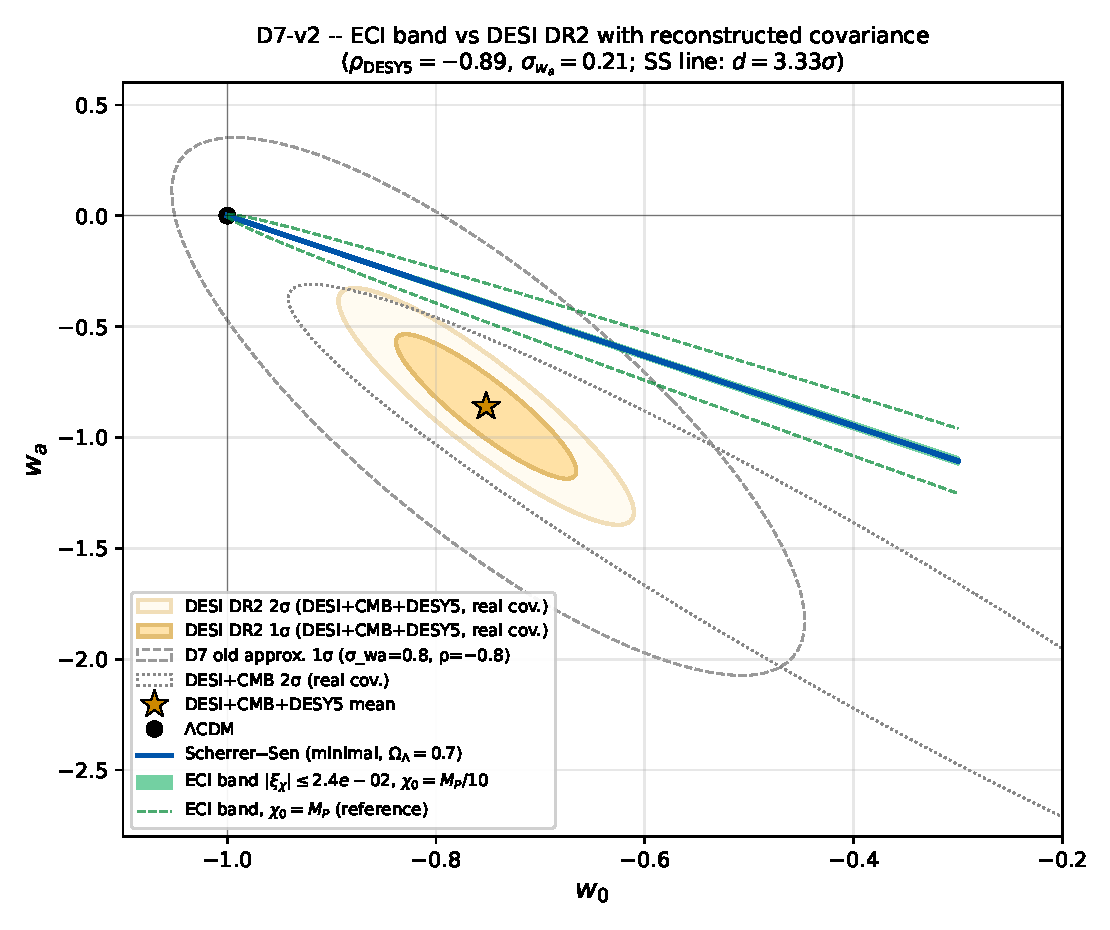
\includegraphics[width=0.95\columnwidth]{../derivations/figures/D7-xi-w0-wa-v2.pdf}
\caption{NMC thawing quintessence in the $(w_0,w_a)$ plane. Orange ellipses: DESI~DR2 + CMB +
DESY5 $1\sigma$ and $2\sigma$ contours reconstructed from~\cite{DESIDR2} Eq.~(28) via the
pivot-redshift identity (see \texttt{D10-desi-covariance.py}; $\sigma_{w_0}=0.057$,
$\sigma_{w_a}=0.215$, $\rho=-0.89$). Blue line: minimal-coupling Scherrer--Sen relation
for $\Omega_\Lambda=0.7$. Green band: ECI NMC prediction with
$|\xi_\chi|\le\xi_{\max}\approx 2.4\!\times\!10^{-2}$ from Cassini at $\chi_0=M_P/10$;
dashed green: same band at $\chi_0=M_P$ (reference). Black dot: $\Lambda$CDM. The ECI band
is $\sim\!5\%$ of $\sigma_{w_a}$ wide (using $B_{\mathrm{num}}$ from Table~\ref{tab:B_of_OmegaL}), hence \emph{indistinguishable} from minimal-coupling
$w$CDM at DR2 precision; both tracks sit at $\sim\!3.3\sigma$ Mahalanobis distance from the
DR2+DESY5 mean.}
\label{fig:D7}
\end{figure}

\paragraph{Honest caveats.}
\begin{enumerate}
\item Eq.~(\ref{eq:gamma_PPN_full}) assumes a \emph{quasi-static} scalar with Compton wavelength
  large compared with the solar system ($m_\chi^{-1}\gg 1\,$AU), which is automatic for the
  ultra-light thawing mass $m_\chi\sim H_0\sim 10^{-33}$\,eV. It also assumes no screening; if
  a chameleon or symmetron mechanism operates, the local $\chi_0$ entering
  (\ref{eq:gamma_PPN_lead}) can differ from the cosmological background and the bound weakens.
\item The NMC Scherrer--Sen extension (\ref{eq:wa_NMC}) is first-order in $\xi_\chi$ and
  therefore \emph{invalid} near the conformal point $\xi_\chi=1/6$, where the expansion breaks
  down and the scalar-tensor sector must be treated non-perturbatively (Einstein-frame
  mapping). Within the Cassini-allowed range $|\xi_\chi|\lesssim 2.4\times 10^{-2}\ll 1/6$
  the linear expansion is controlled. The coefficient $B(\Omega_\Lambda)$ in
  Eq.~(\ref{eq:wa_NMC}) was, in v4.4 of this paper, set by the matter-era
  heuristic ratio $B/A=8/\sqrt3$; in this version we replace that heuristic with
  the full numerical result $B_{\mathrm{num}}(\Omega_\Lambda)$ tabulated in
  Table~\ref{tab:B_of_OmegaL}, obtained from a self-consistent
  NMC-Friedmann + Klein--Gordon integration across $z\in[999,-0.45]$
  (\texttt{derivations/D13-wa-numerical-full.py}). The numerical coefficient is
  nearly flat ($B_{\mathrm{num}}\simeq 9$) across the matter--DE transition
  rather than tracking $A(\Omega_\Lambda)$, so the heuristic
  $(8/\sqrt3)A(\Omega_\Lambda)$ is accurate within 5\% only near
  $\Omega_\Lambda\simeq 0.6$ and undershoots by up to $\sim\!40\%$ at
  $\Omega_\Lambda=0.8$. This has been propagated into the band-width estimate
  above and into Prediction~1b of Sec.~\ref{sec:pred}.
\item The DESI~DR2 + CMB + DESY5 $2\times 2$ covariance is reconstructed from the published
  $(w_0,\sigma_{w_0},w_a,\sigma_{w_a},z_p,w_p,\sigma_{w_p})$ via the pivot-minimisation
  identity $\mathrm{cov}(w_0,w_a)=-(1-a_p)\sigma_{w_a}^2$: no official 2$\times$2 covariance
  matrix has been released by the collaboration at the time of writing. The reconstructed
  $\sigma(w_p)_{\rm pred}=0.0257$ differs from the quoted $0.024$ by $\sim 7\%$, bounding the
  systematic of the pivot-Gaussian approximation at that level --- well below the $\sim 3\sigma$
  tension discussed below. See \texttt{derivations/D10-report.md} for the full cross-check.
\item \textbf{Tension with DR2 + DESY5, stated plainly.} Under the reconstructed DR2 + CMB +
  DESY5 covariance the Mahalanobis distance from the posterior mean is $3.29\sigma$
  (2-dof) to the ECI band and $3.33\sigma$ to the minimal-coupling Scherrer--Sen line,
  both \emph{outside} the $2\sigma$ threshold $\sqrt{6.17}\simeq 2.48$.
  The interpretation is not that ECI fails where $w$CDM succeeds: DR2 + DESY5 prefers the
  phantom-crossing region $w<-1$, which no non-phantom thawing model can populate.
  ECI's NMC coupling $\xi_\chi$ does in principle permit crossing $w=-1$ without a ghost
  instability (established in \S\,DESI DR2 via the no-ghost analysis of Bar\-ce\-l\'o~\&~Visser
  \cite{BarceloVisser2000}), but only at $\xi_\chi(\chi_0/M_P)^2$ values far exceeding the
  Cassini bound~(\ref{eq:xi_bound}) derived here; within the Cassini-allowed range
  the NMC correction to the Scherrer--Sen track is confined to a band of half-width
  $\sim\!5\%$ of $\sigma_{w_a}$ and cannot bridge the gap to the phantom quadrant. The
  $\sim\!3.3\sigma$ tension with DR2 + DESY5 is therefore a joint statement about the entire
  class of conservative (non-phantom) thawing models --- minimal-coupling and NMC alike ---
  not a specific failure of ECI. Prediction~1 in Sec.~\ref{sec:pred} is \emph{not}
  discriminative at DR2 precision; both thawing families sit at the same distance from
  the DR2 + DESY5 posterior.

  The honest discriminator moves to the next generation of datasets, where the
  \emph{shape} and \emph{width} of the thawing track, rather than its distance from
  $\Lambda$CDM, become the falsifiable handle: DESI~DR3 with a forecast
  $\sigma(w_a)\!\sim\!0.07$~\cite{DESIForecast}
  and LSST~Y10 with a forecast $\sigma(w_a)\!\sim\!0.05$
  are in the regime where the ECI NMC band half-width
  $\Delta w_a^{\rm ECI}\sim 1.1\times 10^{-2}$ (numerical, Table~\ref{tab:B_of_OmegaL};
  up from $9\times 10^{-3}$ under the v4.4 heuristic) approaches the
  $15$--$25\%$ level of the statistical error bar and becomes, at least in principle,
  separable from the minimal-coupling Scherrer--Sen locus. The discriminative
  power is slightly larger at $\Omega_\Lambda\gtrsim 0.7$ (DR3 era) because
  $B_{\mathrm{num}}/B_{\mathrm{heur}}$ grows from $0.83$ at $\Omega_\Lambda=0.5$ to
  $1.43$ at $\Omega_\Lambda=0.8$.
\end{enumerate}

The PPN bound (\ref{eq:xi_bound}) is however itself a falsifier: a detection
$|\gamma-1|>10^{-6}$ by the upcoming LATOR or BEACON-class missions, or a mismatch between
$\dot G/G$ from LLR~\cite{Biskupek2021} and the CMB-inferred scalar evolution, would directly
constrain $\xi_\chi(\chi_0/M_P)$ at the $10^{-4}$ level and feed back on the admissible ECI
thawing amplitude.

% -----------------------------------------------------------------------------
% Standalone compile (for checking only):
%   \documentclass[aps,prd,reprint]{revtex4-2}
%   \usepackage{graphicx,amsmath,amssymb,hyperref,physics}
%   \begin{document}\input{section_3_5_constraints}\end{document}
% The \cite{BertottiIessTortora2003}, \cite{ScherrerSen2008}, \cite{DESIDR2},
% \cite{Biskupek2021}, \cite{BarceloVisser2000}, \cite{Wolf2025}, \cite{Ye2025},
% \cite{PanYe2026} keys are defined in eci.bib.
% -----------------------------------------------------------------------------
% section_3_6_swampland_cross.tex — ECI v4.2 scientific payload (D8)
% To be \input{} into eci.tex as a new subsection of §3 "Phenomenology",
% immediately after \input{section_3_5_constraints}.

\subsection{Swampland $\times$ NMC cross-constraint}\label{sec:swampland_cross}

Axioms A4 and A5 were presented as independent. They are not, if the thawing
scalar $\chi$ and the KK tower of the Dark Dimension originate from the
\emph{same} higher-dimensional sector --- a natural hypothesis, since both
are postulated as microscopic ingredients of the dark sector. In that case
both must respect a common effective field theory cutoff $\Lambda$, and the
two axioms are tied by a single consistency condition. The derivation is in
\texttt{derivations/D8-swampland-nmc-cross.py}; we quote only the result.

\paragraph{Shared cutoff.}
The Dark Dimension scenario~\cite{Bedroya2025} relates the EFT cutoff to
the Hubble scale through a Swampland Distance Conjecture exponent,
\begin{equation}
  \Lambda \;\sim\; M_P\,\bigl(H/M_P\bigr)^{c'},\qquad c'\simeq 0.05\pm 0.01.
  \label{eq:Lambda_SDC}
\end{equation}
If the non-minimal operator $(\xi_\chi/2)R\chi^2$ is generated inside the same
EFT, its contribution to the effective reduced Planck mass,
$\delta M_P^{2}=\xi_\chi\chi_0^{2}$, cannot exceed the cutoff squared,
otherwise the operator would repair physics above its own range of validity:
\begin{equation}
  \xi_\chi\,\chi_0^{2}\;\le\;\Lambda^{2}
  \quad\Longleftrightarrow\quad
  \xi_\chi\,(\chi_0/M_P)^{2}\;\le\;(H_0/M_P)^{2c'}.
  \label{eq:eft_bulk}
\end{equation}
Combined with the Cassini PPN bound derived in \S\ref{sec:xi_constraints},
$|\xi_\chi|(\chi_0/M_P)\le 2.4\times 10^{-3}$, Eq.~(\ref{eq:eft_bulk}) yields
at the fiducial thawing amplitude $\chi_0=M_P/10$ and the paper's A5
fiducial $c'=0.05\pm 0.01$
\begin{equation}
  \boxed{\;|\xi_\chi|\;\lesssim\;9.5\times 10^{-5}
    \quad(c'=0.05,\ \chi_0=M_P/10),\;}
  \label{eq:xi_crossbound}
\end{equation}
with an overall range $[5.9\times 10^{-6},\,1.5\times 10^{-3}]$ spanned by
$c'=0.04$--$0.06$. This is a factor $\sim\!250$ tightening over the
Cassini-only result (\ref{eq:xi_max_numeric}).

\paragraph{Limits.}
Both limits verified symbolically in \texttt{D8-swampland-nmc-cross.py}:
$\xi_\chi\!\to\!0$ removes the operator (GR recovered); $c'\!\to\!0$ sends
$\Lambda\!\to\!M_P$ so that (\ref{eq:eft_bulk}) reduces to the no-ghost
condition $\xi_\chi\chi_0^{2}<M_P^{2}$ already stated in A4, and the D7
Cassini bound is recovered exactly.

\begin{figure}[h]
\centering
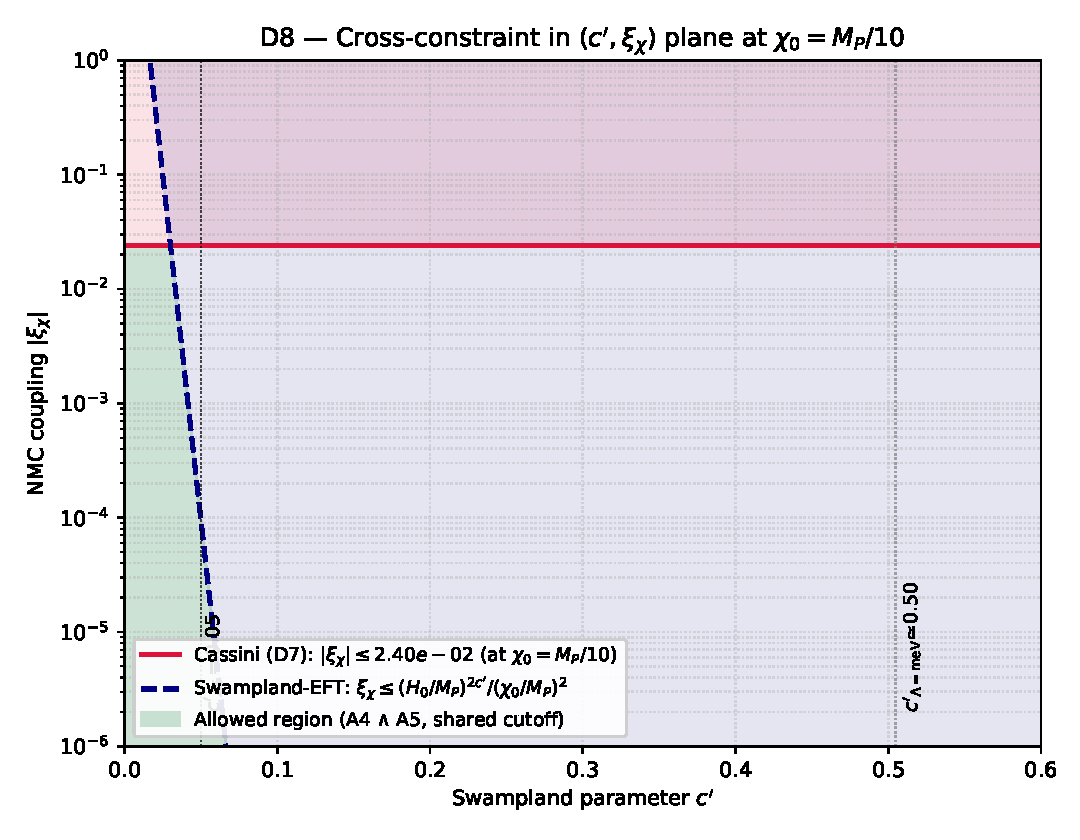
\includegraphics[width=0.95\columnwidth]{../derivations/figures/D8-c-xi-overlap.pdf}
\caption{Allowed region in the $(c',\xi_\chi)$ plane at $\chi_0=M_P/10$.
Red: Cassini exclusion (horizontal, independent of $c'$). Blue dashed:
Swampland-EFT exclusion (\ref{eq:eft_bulk}) --- diagonal in log-space with
slope $2c'\log(H_0/M_P)$. Green shading: overlap admitted by both
constraints. The A5 fiducial $c'=0.05$ and the meV-equivalent value
$c'\!\simeq\!0.51$ are marked.}
\label{fig:D8}
\end{figure}

\paragraph{Phenomenological tension.}
A stronger statement runs in the reverse direction. Thawing dark energy
requires $\chi_0/M_P\sim 0.1$--$1$ to drive late-time acceleration. The
bulk-mode condition (\ref{eq:eft_bulk}) at the Cassini-saturating value
$|\xi_\chi|=2.4\!\times\!10^{-2}$ and $c'=0.05$ forces
$\chi_0/M_P\le 6.3\!\times\!10^{-3}$, already an order of magnitude below
what A4 requires. With the literal Dark Dimension cutoff $\Lambda\sim$ meV
(which the formula (\ref{eq:Lambda_SDC}) reproduces for $c'\simeq 0.51$,
not $0.05$; both conventions appear in the literature) the bound collapses
to $\chi_0/M_P\le 3\!\times\!10^{-30}$ and thawing phenomenology is
excluded outright.

\paragraph{Architectural consequence.}
A4 and A5 are compatible \emph{only} under one of the following model-
building choices, any of which must be made explicit in any UV completion:
(i) $\chi$ is a 4D zero-mode localised on a brane, not a bulk mode of the
same sector as the KK tower, in which case the shared-cutoff hypothesis
does not apply; (ii) a chameleon/symmetron mechanism screens the local
$\chi_0$ away from its cosmological value, weakening the Cassini leg; or
(iii) $|\xi_\chi|$ sits at the sharpened bound (\ref{eq:xi_crossbound})
rather than the Cassini-only value (\ref{eq:xi_max_numeric}). The ECI
framework does not prefer one of the three, but their distinct
phenomenologies are observationally separable: option (iii) suppresses the
ECI band in $(w_0,w_a)$ by a further factor $\sim\!250$ relative to the
already-narrow D7 band, and cuts the $|\dot G/G|$ signature at LLR by the
same factor. A detection of $|\dot G/G|\gtrsim 10^{-17}\,\mathrm{yr}^{-1}$
would rule out option (iii) and force either (i) or (ii).

\paragraph{Honest caveats.}
\begin{enumerate}
\item The EFT self-consistency condition $\delta M_P^{2}\le\Lambda^{2}$ is
  order-of-magnitude; an $O(1)$ coefficient could shift
  (\ref{eq:xi_crossbound}) by a factor $2$, but the qualitative conclusion
  ($\gg 30\%$ tightening) is robust.
\item The form (\ref{eq:Lambda_SDC}) is written with $H$ as the distance
  proxy along the moduli space; the equivalent Bedroya form uses the
  cosmological constant density directly and yields $c'\!\simeq\!1/2$
  for $\Lambda\!=\!$\,meV. The sign of the tightening is independent of
  this choice.
\item The cross-constraint is \emph{conditional} on the shared-cutoff
  hypothesis. Its falsifier is, precisely, the discovery of a UV completion
  in which $\chi$ and the KK tower belong to different sectors; in that
  case §\ref{sec:xi_constraints} remains the strongest bound.
\end{enumerate}

% -----------------------------------------------------------------------------
% Standalone compile (for checking only):
%   \documentclass[aps,prd,reprint]{revtex4-2}
%   \usepackage{graphicx,amsmath,amssymb,hyperref,physics}
%   \begin{document}\input{section_3_5_constraints}\input{section_3_6_swampland_cross}\end{document}
% All \cite{} keys used here (Bedroya2025) are defined in eci.bib.
% -----------------------------------------------------------------------------
\end{document}
% All \cite{} keys used here (Bedroya2025) are defined in eci.bib.
% -----------------------------------------------------------------------------
\end{document}
% All \cite{} keys used here (Bedroya2025) are defined in eci.bib.
% -----------------------------------------------------------------------------
\end{document}
% All \cite{} keys used here (Bedroya2025) are defined in eci.bib.
% -----------------------------------------------------------------------------
